\documentclass[12pt]{report}
\usepackage[utf8]{inputenc}
\usepackage{graphicx}
\graphicspath{{figures/}}
\usepackage[style=numeric]{biblatex}
\usepackage{hyperref}

\addbibresource{references/clustering_algorithms.bib}
\addbibresource{references/research_methods.bib}
\addbibresource{references/reviewed_papers.bib}
\addbibresource{references/microservices_soa_general.bib}
\addbibresource{references/software_clustering.bib}
\addbibresource{references/static_analysis.bib}
\addbibresource{references/other.bib}
\addbibresource{references/semantic_analysis.bib}

% For setting the page layout
\usepackage[a4paper,width=150mm,top=25mm,bottom=25mm,bindingoffset=10mm]{geometry}
% For spacing
\usepackage{setspace}
%\singlespacing
\onehalfspacing
%\doublespacing
% For the style of the pages
\usepackage{fancyhdr}
\newcommand{\changefont}{%
    \fontsize{9}{11}\selectfont
}
\fancyhf{}
\fancyhead[LE]{\slshape \rightmark} %section
\fancyhead[RE]{\thepage}
\fancyhead[RO]{\slshape \leftmark} % chapter
\fancyfoot[C]{\changefont \thepage} %footer
\pagestyle{fancy}
% To color table cells
\usepackage[table]{xcolor}
% For plots
\usepackage{pgfplots}
% For boxplot
\usepgfplotslibrary{statistics}
% To adjust the width of tables:
\usepackage{array}
% To get the commands \toprule and \cmidrule:
\usepackage{booktabs}
% To control captions, e.g. centering them:
\usepackage{caption}
% To make network graphs
\usepackage{tikz-network}
% For subfigures
\usepackage{subcaption}
% To turn a page to landscape mode
\usepackage{rotating}
% For code snippets
\usepackage{listings}
% For matrices and vector notation
\usepackage{amsmath}
% For defining algorithms
\usepackage{algorithm2e}
\usepackage{algorithm}
\usepackage{algorithmic}
% For creating subtables and subfigures
\usepackage{caption}
\usepackage{subcaption}
% For shapes in graphs
\usepackage{tikz}
% for multi rows in tables
\usepackage{multirow}
% For table positioning
\usepackage{float}
% For tree
\usepackage{qtree}
% For centering overfull tables
\usepackage{adjustbox}

\setcounter{tocdepth}{1} % Show sections
%\setcounter{tocdepth}{2} % + subsections
%\setcounter{tocdepth}{3} % + subsubsections
%\setcounter{tocdepth}{4} % + paragraphs
%\setcounter{tocdepth}{5} % + subparagraphs

\definecolor{CellGray}{HTML}{C0C0C0}
\definecolor{LightGray}{HTML}{f6f6f6}
\definecolor{codegreen}{rgb}{0,0.6,0}
\definecolor{codegray}{rgb}{0.5,0.5,0.5}
\definecolor{codeorange}{HTML}{b5722f}

\lstdefinestyle{code_snipped_style}{
    backgroundcolor=\color{LightGray},   
    commentstyle=\color{codegreen},
    keywordstyle=\color{codegreen},
    numberstyle=\tiny\color{codegray},
    stringstyle=\color{codeorange},
    basicstyle=\ttfamily\footnotesize,
    breakatwhitespace=false,         
    breaklines=true,                 
    captionpos=t,                    
    keepspaces=true,                 
    numbers=left,                    
    numbersep=10pt,                  
    showspaces=false,                
    showstringspaces=false,
    showtabs=false,                  
    tabsize=2
}

\lstset{style=code_snipped_style}

\captionsetup{format=plain, font=small, labelfont=bf, margin={2.5cm,0cm}}
%\captionsetup{justification=normal, margin={2.5cm, 1.5cm}, labelfont=bf, font=footnotesize}

\begin{document}
\begin{titlepage}
    \begin{center}
    
    \vspace*{2cm}
    UTRECHT UNIVERSITY
    
    \vspace*{2.5cm}
    
    {\Huge \textbf{From a Monolith to Microservices:}}
    
    \vspace{0.6cm}
    
    {\Huge \textbf{the Effect of Multi-view Clustering}}
    
    \vspace{0.5cm}
    
    {\small \textit{FINAL VERSION}}
    
    
    \vspace{1.5cm}
    
    {\Large By}
    
    \vspace{0.4cm}
    
    {\Large Lars M.A. van Asseldonk}
    
    \vspace{1cm}
    
    6970907\\
    \href{mailto:l.m.a.vanasseldonk@students.uu.nl}{l.m.a.vanasseldonk@students.uu.nl}
    
    \vfill
    
    1st Supervisor: Dr. J. (Jurriaan) Hage \\
    2nd Supervisor: Dr. ir. J.M.E.M. (Jan Martijn) van der Werf
    
    \vspace{2cm}
    
    Business Informatics\\
    Graduate School of Natural Sciences\\
    
    \vspace{1cm}
    
    \today
    
    \end{center}
\end{titlepage}

\pagenumbering{roman}

\thispagestyle{plain}
\begin{center}
    UTRECHT UNIVERSITY
    
    \vspace*{0.4cm}
    
    \Large
    \textbf{From a Monolith to Microservices:\\ The Effect of Multi-view Clustering}
        
    \vspace{0.4cm}
    
    \large{By}
    
    \vspace{0.2cm}
    
    \large{Lars M.A. van Asseldonk}
       
%    \vspace{0.2cm}
    \section*{Abstract}
\end{center}

In today's demanding world, many companies migrate their monolithic systems to a microservices landscape. The most costly task in this process is refactoring the application into a suitable set of microservices. Decomposition techniques help the architect to understand better how the intended microservices architecture can be designed. These techniques take the monolithic system as input and output a set of candidate microservices. Over the years, many microservice decomposition techniques have been proposed. 
Most of these techniques focus on one viewpoint of the system, such as its static or dynamic behaviour, even though it is perfectly possible to combine them. 
To the best of our knowledge, we did not find any research that measures the effect of incorporating multiple viewpoints of the system on the quality of the microservices decomposition. 
This thesis studies the effect of multiple viewpoints based on the rationale that extra information results in a better decomposition. To do this, we developed a Python tool that extracts static, semantic, and dynamic dependencies from a monolith and represents them in an edge-weighted graph. 
A graph algorithm (Louvain) is then used to find communities in the graph that are highly connected and loosely coupled. We validate our approach by applying our tool to seven open-source Python projects. The quality of the resulting decompositions is then measured and compared in terms of functional independence and structural and conceptual modularity quality. The results show that incorporating multiple views of the system does not gradually increase the quality of the decomposition. However, combining static and dynamic information does result in a better decomposition in terms of modularity quality compared to the use of static or dynamic information individually. When semantic information is involved, we noticed that the decomposition quality significantly decreases for three metrics (IFN, OPN and, SMQ). 
This pattern could be justified by the fact that semantic decompositions contain much more dependencies, and therefore tend to favor semantics while focussing less on static and dynamic dependencies.
\addcontentsline{toc}{chapter}{Abstract}

\tableofcontents
\clearpage

\listoffigures
\addcontentsline{toc}{chapter}{List of Figures}
\clearpage

\listoftables
\addcontentsline{toc}{chapter}{List of Tables}
\clearpage

\pagenumbering{arabic}

\chapter{Introduction}\label{c:introduction}
Over the years, the architecture of many large applications has evolved from monoliths to microservices in order to make the IT environment more flexible and responsive to today's fast-changing business requirements. The microservices architecture, inspired by the principles of Service-Oriented Architectures (SOA) \cite{dragoni2017yesterday}, consists of small autonomous applications that communicate together with lightweight mechanisms like HTTP requests. A microservice is a standalone application that can be independently deployed, scaled, and tested and has a single responsibility \cite{thones2015microservices}. This means that a microservice should be fully controlled and owned by a single team. To better understand the fundamentals of microservices, we first discuss the notion of monolithic systems. \par
In a monolith, all code is combined into a single executable. A monolith is relatively easy to build, but when the application gets bigger, it becomes difficult to understand and maintain the code. \citeauthor{fritzsch2019microservices} \cite{fritzsch2019microservices} researched the intentions, strategies, and challenges of microservices and found out that the main driver to migrate from a monolith to microservices is the lack of code maintainability. The lack of maintainability often occurs when the codebase becomes too big, making it difficult for developers to keep track of changes. \citeauthor{kalske2017challenges} \cite{kalske2017challenges} define three drivers for migrating to microservices, namely: a high number of teams, a big codebase, and teams geographically located far from each other. When none of the aforementioned drivers exists, microservices might not be the most appropriate solution. According to \cite{kalske2017challenges}, it is preferred to start with a monolith in order to avoid technical and organisational challenges that microservices bring. For this reason, most companies start with a monolith and iteratively migrate towards a microservices architecture when the codebase becomes unmanageable \cite{fritzsch2019microservices, kalske2017challenges}. \par 
\section{Problem statement}\label{s:problem}
Refactoring the monolith into microservices is a daunting and costly task that takes a lot of time and effort from the organisation \cite{kalske2017challenges}. One of the biggest challenges is to find the right service cuts in the software \cite{fritzsch2019microservices}, as many variations are possible. Over the years, the scientific community has published many decomposition techniques that help organisations automatically identify microservice boundaries. Most of these approaches only rely on one viewpoint of the system, such as the source code, runtime environment, or design elements. Even though it is feasible to combine different sources of information without any problems. A literature review by \citeauthor{ponce2019migrating} \cite{ponce2019migrating} also states that \textit{more evidence of mixed proposals is needed}. In this research, we will build upon this observation. \par
To the best of our knowledge, we have not found any decomposition approach that collects structural dependencies and semantic information hidden in the source code and runtime information to identify suitable microservices. This research fills that gap and contributes to the academic community by building a framework that combines these three information sources. Furthermore, we want to discover the relationship between the availability of different sources of information and the quality of the decomposition. 
In terms of contribution to practice, we give organisations insights into the use of different information sources incorporated in the decomposition process. For example, if an organisation only has dynamic information at its disposal, we give an understanding of how this probably will affect the quality of the decomposition.

\section{Aim}
The goal of this research is to understand the effect of incorporating multiple sources of information on the quality of the microservice decomposition. The rationale behind this is that extra information results in a better decomposition. We also aim to find out which source is most informative and which combinations are most powerful. 
%If time allows, we want to expand the experiment by applying different classes of clustering algorithms to understand how this is associated with the incorporated degree of information. 

\section{Research questions}
Following the two aforementioned research objectives, we have constructed the following Main Research Question (MRQ). The MRQ is subsequently divided into several Sub Questions (SQ).

\begin{itemize}
    \item[$MRQ$] What is the effect of combining static, dynamic and semantic sources of information extracted from monolithic software on the quality of the discovered microservices?
\end{itemize}
\begin{itemize}
    \item[$SQ_1$] What is currently known about static, dynamic and semantic data extracted from monolithic software?
    \item[$SQ_2$] What algorithms are commonly used for the task of microservice identification?
    \item[$SQ_3$] What measures are used in the literature to define the quality of a decomposition?
    \item[$SQ_4$] What is the decomposition quality when incorporating only a single source of information? 
    \item[$SQ_5$] How does the quality of the decomposition change when incorporating multiple sources of information?
\end{itemize}

\subsection{Research context}
For the reader, it is important to know in which context the research is conducted. Therefore, we briefly discuss some design decisions that are made throughout this research.\par
Firstly, the technology stack in which the approach is implemented. Due to personal experiences, we have chosen to implement the approach in a Python context. This means the approach will only be compatible with applications that are written purely in Python. An advantage of executing the research in a Python context is that we differentiate ourselves from others, as most of the existing work presented in the literature review (Section \ref{s:literature_results}) is based on Java applications. However, the downside of this decision is that we are not able to compare the results of our approach to state-of-the-art techniques, as none of them uses Python. \par
Secondly, we will validate our approach with open-source applications. This way, everyone has access to the source code leading to results that are easier to replicate. The risk of this decision is that we only validate the technique on relatively small applications. Also, the results cannot be validated with expert opinions. 
\section{Research method}\label{s:method}
The research method that we use throughout this research relies on characteristics of Design Science (DS). Design science is one of the main research paradigms in the Information Systems (IS) discipline \cite{hevner2004design}. The paradigm focuses on the creation and evaluation of IT artifacts that aim to solve identified organisational problems \cite{hevner2004design}. There exist many IS design science frameworks in the current literature, and they all have small adaptations. \citeauthor{offermann2009outline} \cite{offermann2009outline} conducted a comparison of design science methodologies and discovered three main phases: (1) problem identification, (2) solution design, and (3) evaluation. \par

Throughout this research, we follow the Design Science Research Methodology (DSRM) introduced by \citeauthor{peffers2007design} \cite{peffers2007design}. There are three reasons for choosing this methodology. First, the methodology has an objective and scientific nature \cite{venable2017choosing}. This means, e.g., that the problem statement is mostly based on literature and not derived from subjective opinions from stakeholders. Moreover, the DSRM method is made for IS research that aims to design artefacts that are tools or techniques rather than products or processes \cite{venable2017choosing}. In this research, we aim to design such a technique. At last, the methodology does not consider the designed artefact to be implemented in the real world \cite{venable2017choosing}, which is in line with our research. \par

The DSRM is synthesised from seven other design science methods and consists of six activities executed in a nominal sequence. Table \ref{tab:research_approach} gives an overview of the steps and the related research methods and questions. The activities are described below. \par

\begin{table}[h]
    \small
    \caption[Overview of research process]{Overview of the research process and the related research questions and methods that are used.}\label{tab:research_approach}
    \begin{tabular}{>{\raggedright}m{75pt} >{\raggedright}m{107pt} >{\raggedright}m{60pt} >{\raggedright\arraybackslash}m{100pt}}
        \toprule
        Phase by Offerman et al. 
        & Activities by Peffers et al. 
        & Question(s) 
        & Research Method \\
        \midrule
        Problem Identification 
        & Problem identification and motivation 
        & SQ1
        & Literature Study I \\
        & Define the objectives for a solution 
        & SQ2, SQ3 & Literature Study II \\
        \midrule
        Solution Design 
        & Design and development
        & -
        & Prototyping \\
        \midrule
        Evaluation 
        & Demonstration 
        & SQ4, SQ5
        & Experiment I \\
        & Evaluation & MRQ & Experiment I \\
        \midrule
        - & Communication & MRQ & - \\
        \bottomrule
    \end{tabular}
\end{table}

% h = float specifier
% 312pt is the full-width of the table

\begin{itemize}
    \item \textbf{Problem identification and motivation.} During the problem investigation phase, the goal is to \textit{specify the research problem and justify the value of a solution} \cite{peffers2007design}. This is done by conducting a systematic literature review. This first literature review is needed to collect and review the state-of-the-art concerning the decomposition techniques. The literature review, presented in Chapter \ref{c:related_work}, results in a problem statement (see Section \ref{s:problem}) in which the importance of the solution is clarified.
    \item \textbf{Define the objectives for a solution.} In the next phase, the objectives of the designed artefact are defined. To do this, we perform a second literature review in which potential solutions are studied in a semi-systematic way. For instance, we look thoroughly into clustering algorithms that are particularly used in this domain in order to collect requirements. Furthermore, we define the context in which the solution is executed. This means, e.g., we examine tools and libraries to extract data from the monolith and define which applications are suitable to validate the technique. We also use the results of the first literature review to get insights into the state-of-the-art. 
    \item \textbf{Design and development.} In this phase, we design and develop a prototype of the multi-view decomposition technique. The prototype is verified on toy examples in order to prove it works as intended. Chapter \ref{c:multi-view_clustering} describes how the multi-view clustering tool is developed, and the design decisions that are made during the process.
    \item \textbf{Demonstration.} In the demonstration step, the multi-view clustering tool is validated in a more realistic context. The applications found during the second literature review are used to demonstrate the working of the prototype on another \textit{instance of the problem} \cite{peffers2007design}. To do this, we apply the tool on seven open-source projects. For each project, the tool extracts static, semantic, and dynamic dependencies used to decompose the system. As input for the decomposition, we use three different levels of information: a single data source, a pair of data sources, and all the data sources. This leads to a total of seven distinct decompositions. An overview of the experiment is presented in Table \ref{tab:experimental_design}. The stars ($*$) in the table indicate which source of information is active in each group.
    \begin{table}[h]
\centering
    \caption[Experimental design]{Experimental design. Each star (*) in the table indicates the appearance of the data source while an empty cell shows the absence of the data.}\label{tab:experimental_design}
    \begin{tabular}{c|c|c|c|c|c|c|c|}
        \cline{2-8}
        & \multicolumn{7}{c|}{Experiments}\\
        \cline{2-8}
        & 1 & 2 & 3 & 4 & 5 & 6 & 7 \\
        \hline
        \multicolumn{1}{|c|}{Static} & * & & & * & & * & *\\
        \hline
        \multicolumn{1}{|c|}{Dynamic} & & * & & * & * & & *\\
        \hline
        \multicolumn{1}{|c|}{Semantic} & & & * & & * & * & *\\
        \hline
        & \multicolumn{3}{c|}{Single} & \multicolumn{3}{c|}{Pair} &  \multicolumn{1}{c|}{All}\\
        \cline{2-8}
    \end{tabular}
\end{table}
    %\begin{table}[h]
    \small
    \caption[Experimental design]{Experimental design. Each star (*) in the table indicates the appearance of the data source while an empty cell shows the absence of the data.}\label{tab:experimental_design}
    \begin{tabular}{r|c|c|c|c|c|c|c}
        \toprule
        \multirow{3}{*}{Information used}& \multicolumn{7}{c}{Experiments}\\
        \cmidrule{2-8}
        & \multicolumn{3}{c|}{Single} & \multicolumn{3}{c|}{Pair} &  \multicolumn{1}{c}{All}\\
        \cmidrule{2-8}
        & 1 & 2 & 3 & 4 & 5 & 6 & 7 \\
        \midrule
        Static dependencies & * & & & * & & * & *\\
        \midrule
        Semantic similarity & & * & & * & * & & *\\
        \midrule
        Dynamic dependencies & & & * & & * & * & *\\
        \bottomrule
    \end{tabular}
\end{table}
    \item \textbf{Evaluation.} In the evaluation step, we analyse the different decompositions collected from the experiment in order to quantify the quality of the decomposition. The different decompositions are compared to each other in order to gain an understanding of the effect of information sources on the quality of the decomposition. The evaluation is done by microservice specific measures that are researched and selected during the second literature review. 
    \item \textbf{Communication.} In the last phase, we present the research results to interested fellow students and, depending on the quality, made it ready for a scientific publication.
\end{itemize}


\chapter{Background}\label{c:background}
Before we dive into related decomposition techniques, it is crucial to have a solid understanding of the research domain. This section introduces important concepts that are used throughout the research domain such as software clustering in general, microservices, the monolith, the kinds of sources of information we can extract from the monolith and clustering algorithms.

\section{Software clustering}\label{s:software_clustering}
Decomposing monolithic software into a suitable set of microservices is based on the idea of software clustering. Software clustering is the general task of grouping software entities based on their interrelationships or similarity. These software entities could represent more detailed functions and their invocations (low-level entities) or more abstract packages, modules and files (high-level entities), depending on the level of detail desired in the clustering \cite{alsarhan2020software}. Software clustering is an old domain of research as one of the first papers published \cite{belady1981system} dates back to 1981. Over the years, software clustering has shown its potential in various application areas, for example, to identify fault proneness or to locate code fragments that implement related functionality \cite{alsarhan2020software}. Another popular software clustering aim is to reduce the system's complexity by splitting up the system into smaller independent chunks of software \cite{wiggerts1997using}. This way, the software becomes less complex, allowing developers to more easily maintain and add new functionality to the software. In this study, we focus on software clustering techniques that aim to identify microservice boundaries in monolithic software.\par
Automatic clustering of software is a challenging task and knows two fundamental problems. The first problem indicates that there are too many unique ways of decomposing software. A paper by \citeauthor{mancoridis1998using} \cite{mancoridis1998using} shows that the number of unique decompositions grows exponential with respect to the number of classes in the source code. This first problem is considered a search problem and is further discussed in Section \ref{s:clustering_algorithms}. The second problem of software clustering is the ambiguity in measuring the quality of a good decomposition. One of the reasons for this is that there is no ideal solution that fits every scenario. Instead, the decomposition quality depends on many factors, such as the organisation structure and the desired granularity. Over the years, many validation metrics have been introduced that aim to quantify either specific microservice decompositions \cite{jin2018functionality} or decompositions in general \cite{mitchell2001craft}. We elaborate on this in Section \ref{s:literature_results}. \par

\section{The monolith}
As mentioned in the introduction, a monolith is a software application in which all the code is combined into a single executable file. \citeauthor{dragoni2017yesterday} \cite{dragoni2017yesterday} defines a monolith as a system \textit{whose modules cannot be executed independently.} The modules are dependent on each other because they rely on shared resources such as databases, files or memory. The monolith suffers from several issues \cite{dragoni2017yesterday}:

\begin{itemize}
    \item hard to maintain when codebase becomes too big
    \item "dependency hell"
    \item a small change requires redeploying the whole system
    \item due to conflicting requirements a 'one-size-fits-all' deployment configuration
    \item limited scalability
    \item technology lock-in for developers
\end{itemize}

To cope with these limitations, the Service-Oriented Architectural (SOA) style has been introduced. In SOAs, software entities interact with other entities via message passing communication \cite{dragoni2017microservices}. Microservices are closely related and have been introduced by the industry due to the fact that the service-oriented paradigm did not give clear requirements on how to design them well \cite{dragoni2017yesterday}. There was a lack of consensus on how to get a well-defined SOA \cite{newman2015building}. For this reason,  some practitioners argue that microservices are a particular way of implementing of SOAs \cite{zimmermann2017microservices}, and therefore do not represent a new architectural style. We can say that microservices are a way of designing service-oriented architectures. In this study, we focus on microservices.

\section{Microservices}\label{s:microservice_principles}
Microservices are described by \citeauthor{newman2015building} \cite{newman2015building} as \textit{"small autonomous services that work together, modelled around a business domain"}. Microservices work independently from each other to ensure that a change in one service can be made without affecting other services. \citeauthor{dragoni2017yesterday} \cite{dragoni2017microservices} defines a microservice as \textit{a cohesive, independent process interacting via messages}. The term \textit{cohesive} indicates that the service only implements functionalities that are strongly related to each other. The microservices architecture is built around a few basic principles \cite{dragoni2017microservices}:

\begin{itemize}
    \item \textbf{Bounded context.} The bounded context, introduced by \citeauthor{evans2004domain} \cite{evans2004domain}, says that each microservice should implement a single business capability. This way, the system structure and business are perfectly aligned.
    \item \textbf{Size.} The microservices have to be small-sized. The small size brings major benefits in terms of maintainability and extendability. However, determining the right level of granularity appears to be a complicated issue \cite{di2018migrating, kalske2017challenges, newman2015building}. In \cite{newman2015building, selmadji2018re}, they refer to the small size as the single responsibility principle (SRP). The SRP states that each service should be focused only on one functionality.
    \item \textbf{Independency.} Microservices have to operate independently from each other. Independence between microservices is achieved by following the loose coupling and high cohesion principle. Furthermore, communication between microservices should only be through published interfaces. In \cite{selmadji2018re}, each microservice should also maintain its own database. 
\end{itemize}

Notice that more microservice principles exist such as being \textit{technology neutral} or \textit{automatically deployable} \cite{selmadji2018re}. However, these are not related to the structure and behaviour of microservices and therefore considered irrelevant for this study. \par

\section{Extracting data from the monolith}\label{s:information_views}
To make a proper decomposition of the monolith, we must have a sufficient amount of information about the monolith. We need to know its structure and how it behaves to define good microservice boundaries. There are various ways to collect relevant information. A literature study by \citeauthor{ponce2019migrating} on decomposition techniques outlines three categories: \textit{model-driven}, \textit{static analysis} and \textit{dynamic analysis}. Next to this, we also consider a fourth category called \textit{evolutionary analysis}. The static analysis is divided into \textit{dependency analysis} and \textit{semantic analysis}. This section is structured according to this division.

\subsection{Model analysis}
Model-driven approaches use system \textit{design elements} as input for the decomposition. System design elements provide documentation about the system and can be represented in many different ways, e.g., domain entities, use-case diagrams or data flow diagrams. The existence of design elements is not guaranteed as it depends on the company. Different companies might use different modelling techniques. For this reason, \citeauthor{gysel2016service} \cite{gysel2016service} developed a technique that allows nine different representations of the system as input. If multiple design elements are available, it is also possible to combine them. To illustrate this better, we give an example based on class diagrams. Class diagrams represent both the structural and behavioral  features of the system. A simple association relationship between two classes tells us there is some dependence. This dependence is described as \textit{semantic proximity} by \cite{gysel2016service} as the two have a semantic connection given the business domain. Two classes that have  strong semantic proximity should be modelled in the same microservice. In the end, the resulting information extracted from the chosen design elements is represented in an undirected weighted graph. To automate the approach, they require the design elements to be in a machine-readable format. \par 
Another design element that can be used is a data-flow diagram (DFD). Data-flow diagrams give a good representation of the business processes of the monolith \cite{chen2017monolith}. A DFD shows how the data flows through the system. Having this knowledge, we can discover, e.g. functions that make use of the same datastore and thus have some relation. Two approaches that use data-flow diagrams for deriving microservices are \cite{chen2017monolith, selmadji2020monolithic}. It is also possible to use business processes as input for the decomposition. In \cite{daoud2020towards} business processes modelled in BPMN notation are used to extract control (execution order), semantic (functional similarity), data (information sharing) and organisational (cross-functional operations) dependencies. \par 
A limitation of model-based approaches is that the used artefacts or documentation can be unavailable or not up to date.

\subsection{Dependency analysis}
In a dependency analysis, structural code dependencies are extracted from the source code. Structural code dependencies capture direct dependencies between two code entities \cite{beck2011congruence}. An example of such direct dependency is: method A calls method B, or class X extends class Y. Often, structural dependencies are represented in a directed graph (also called call graph) \cite{alsarhan2020software}. The dependency graph consists of nodes and edges. The nodes represent the system's modules (e.g. files, classes, functions) while the edges represent their relationship (e.g. function calls, inheritance relationship). The dependency graph is also able to show the strength of the relationship between two code entities. This strength is expressed in weight terms. In \cite{matias2020determining} the weights are calculated by looking at the number of imports and method calls between two components.\par
The structural dependencies might also be valuable to discover indirect relationships among code entities. This can be done by considering the structural dependencies of a code entity (e.g. function) as a feature vector. The rationale behind this is that the similarity between two feature vectors indicates that the two code entities have a similar purpose or functionality. These indirect dependencies are also called the \textit{fan-out similarity (FO)} \cite{beck2011congruence}.\par
A limitation of techniques that focus on structural dependencies is that they rely on a strong assumption that the system is well designed according to software engineering principles. However, for many systems, this is not the case \cite{saeidi2015search}.

\subsection{Semantic analysis}
In semantic analysis, the source code is interpreted as plain text documents \cite{beck2011congruence}. For each code file, a vocabulary is built representing the linguistic information that is embedded in the source code, such as identifier names and comments. This information could be relevant, assuming that similar vocabularies indicate some degree of relation. \par
Each code file is modelled as a bag-of-words vector that shows the occurrence of each term in a document. All the documents together represent a term-document matrix. A successful technique that analyses relationships between documents in the term-document matrix is Latent Semantic Indexing (LSI). In LSI, the term-document matrix is weighted to balance out scarce and ubiquitous terms. Next, singular value decomposition (SVD) is used to reduce the vector space model's dimensions. The similarity in a LSI vector space model is typically defined as the cosine between two vectors. The LSI allows us to compute document-document, term-document and term-term similarities. \par
A risk of semantic analysis is that its success heavily depends on the quality of source code naming \cite{saeidi2015search, alsarhan2020software}. The analysis does not work when developers do not comply with comments and naming conventions. Some companies even anonymise identifier names in the source code to deal with security issues.

\subsection{Dynamic analysis}
In dynamic analysis, the system functionalities are analysed at runtime. To analyse the system at runtime, operational data represented in log files are necessary. A log (execution) file contains information such as a timestamp, the invocated function and its arguments and an optional message. The information obtained from the analysis tells us how the dependencies are exercised during executions and how the system works in reality. For example, we can discover how frequent two function call each other and thereby determine the strength of their relationship. Furthermore, because of the timestamp in the execution log, we know in which order functions are executed. We could use this information when assuming that functions executed close to each other have some relationship. The extracted information from dynamic analysis could be represented in a weighted dependency graph. It is also possible to use the information to update the weights in the dependency graph derived from static analysis \cite{matias2020determining}. \par
A possible limitation of dynamic analysis is that changes in the source code are required when operational data is not automatically captured \cite{alsarhan2020software}. To let systems record execution logs, they need to be instrumented and redeployed again. However, when the new instrumented system could not run for a sufficiently long time, there is a risk that the log files do not represent all aspects of the system. To cope with this problem, it is important to have a suitable set of test cases available that simulate as many aspects of the system as possible. 

\subsection{Evolutionary analysis}
Evolutionary analysis aims to extract relevant information that is paired with the evolution of software \cite{beck2011congruence}. This means that we look at how the software changes over time. When two code entities appear to frequently change together during development, this reveals an implicit relationship. Evolutionary data is often managed by a version control system (VCS) such as Git. In version control systems, the change history of a particular project is captured revision logs. A revision log contains information about the code change, such as the author, date and changed files. \par 
Analysing revision logs gives us important insights into the relationships between code entities. For example, as mentioned before, we could identify code entities that frequently change together. Furthermore, since the author who changes the code is known, we can also look at the ownership of code \cite{beck2011congruence}. When two code entities are owned by the same author(s), they might be covered by the same expertise and thus represent some relationship. \par
A limitation of the evolutionary analysis is that change information is not always properly documented. Furthermore, to cover all the parts of the system, a huge set of evolutionary data is necessary \cite{alsarhan2020software}. Dealing with this amount of data is a challenging task. 

\section{Clustering algorithms}\label{s:clustering_algorithms}
Based on the extracted data mentioned in the previous sections, the software has to be clustered into a set of microservices. Clustering is an unsupervised learning task in which data points that are closely related to each other are grouped together. In this section, we describe three classes of clustering algorithms that are commonly used in the process of decomposing monolithic software, namely: \textit{graph-based clustering}, \textit{hierarchical clustering} and \textit{genetic-based clustering}.

\subsection{Graph-based clustering}
Graph-based algorithms partition an undirected graph into sub-graphs. This way, the algorithm does not start from individual data points but tries to find sub-graphs according to some algorithm-specific criteria \cite{wiggerts1997using}. This means that the sub-graphs are forming the clusters. In these graphs, each node represents a code entity, and an edge represents their relationship. Graph-based clustering can be seen as a kind of \textit{partitioning method} since it relocates instances from one cluster to another, starting from an initial partitioning \cite{rokach2005clustering}. \par
To achieve global optimisation in graph-based clustering, an exhaustive search of all possible partitions is required. However, since this is often not feasible due to the large search space, greedy search heuristics are often used \cite{rokach2005clustering}. \par 
A widely used graph-based clustering technique is the Girvan-Newman algorithm \cite{girvan2002community}. This algorithm is often used to identify microservices \cite{gysel2016service, matias2020determining}. In \cite{lohnertz2020steinmetz}, seven graph-based clustering algorithms are compared on the task of decomposition the monolith. Another graph-based clustering technique that is used in previous decomposition studies is the minimal spanning tree (MST) \cite{mazlami2017extraction}. 
An advantage of graph-based algorithms is that they do not require to set the number of clusters.

\subsection{Hierarchical clustering}
Hierarchical clustering is a non-stochastic technique that builds clusters by recursively partitioning instances in either top-down (divisive) or bottom-up (agglomerative) fashion \cite{rokach2005clustering}. In \textit{agglomerative hierarchical clustering}, each data point (code entity) start with its own cluster (singletons). Then, in each step, the two most similar clusters are successively merged until the desired cluster structure is obtained. On the other hand, in \textit{divisive hierarchical clustering} all the data points are represented in one cluster. In each step, the cluster is divided into suitable subclusters, until again a desired cluster structure is obtained. The result of a hierarchical algorithm is typically visualised in a \textit{dendrogram}. To obtain clusters from the dendrogram, a \textit{cutting point} needs to be determined. Note that different cutting points will lead to different clusters. Agglomerative hierarchical algorithms are more often used than divisive algorithms. This is because it is infeasible to consider each possible divisions from the initial cluster. The complexity of hierarchical algorithms depends linearly on the number of classes in the system \cite{kebir2012comparing}.\par 
An advantage of hierarchical clustering is that the algorithm reveals a hierarchy within the data. This information is often more insightful compared to 2-D clusters. Furthermore, the algorithm does not need any apriori information regarding the number of clusters. 

\subsection{Genetic-based clustering}
Genetic algorithms (GA) belong to the class of evolutionary algorithms (EA) and are inspired by concepts of natural selection such as mutation, crossover and selection. Even though there are many variations of GAs, the overall process stays the same. Genetic algorithms start with randomly initialising a \textit{population} of candidate solutions. In GA terminology, a candidate solution is called an \textit{individual} and the set of individuals in a particular iteration is considered a \textit{generation}. After obtaining the initial generation, an iterative process starts in which the fitness of every individual is evaluated based on a predefined \textit{objective function}. A new generation is created by randomly taking the fittest individuals of previous generations. This selection is based on evolution theory, in which only the strongest species survive. The selected individuals for the next generation are modified by applying GA operators such as \textit{crossover} and \textit{mutation}. Typically, the GA stops when a maximum number of generations is produced or when a satisfactory fitness level has been reached for the population. \par
Genetic algorithms are considered beneficial when there is a multi-objective optimisation problem. They perform surprisingly good in highly constrained problems, where the number of good solutions is relatively small compared to the search space \cite{Doval1999}.


\chapter{Related work}\label{c:related_work}
In this section we conduct a literature review to analyse techniques that present a novel way to decompose monolithic software into microservices. This section first explains the utilised search strategy and justifies the qualitative assessment used to characterise the discovered papers. After this, we dive into the results of the literature study.

\section{Search strategy}\label{s:search_strategy}
To start the search process, we have formed the following search string: 

\begin{itemize}
    \item[] \textit{("microservice*" OR "micro-service" OR "micro service") [AND "monolith"] [AND ("refactor" OR "transform" OR "migrat*" OR "decompos*" OR "partition*")]}
\end{itemize}
This search string is a mix of the ones used in \cite{fritzsch2018monolith} \cite{ponce2019migrating} and tells us that the body of the source needs to contain at least the words "microservices" (or one of its variations), "monolith" and "refactor" (or one of its synonyms). \par
The search queries are conducted on the three most frequently used computer science scientific libraries and indexing systems \cite{fritzsch2018monolith}: ACM Digital Library, IEEE Xplore, and Google Scholar. We have chosen these libraries since they have been proven to be most relevant for literature reviews in the software engineering domain \cite{petersen2015guidelines}. \par
To limit the results, we have created certain selection criteria. At first, the articles need to be peer-reviewed and written in English. Moreover, the abstract of the article needs to clearly show that it proposes a novel microservices decomposition technique with some degree of automation. This means that techniques that aim to search for candidate microservices manually are excluded from the review. At last, sources that do not perform static (e.g. dependency or semantic analysis) or dynamic analysis to aggregate input data for the decomposition process are filtered out. This means that model-driven techniques that only take design elements as input are excluded from the literature review. Also, techniques that exclusively focus on evolutionary data are not selected in the literature review. \par
We also have employed snowballing to make sure all the relevant articles are found. The snowballing procedure is recommended by \citeauthor{wohlin2014guidelines} \cite{wohlin2014guidelines} for literature reviews and has two variants. The first one, forward snowballing, identifies new papers that have cited the examined paper. The other one, backward snowballing, finds older papers that are referred by the examined paper. The literature review was conducted on the first of March 2021, and the results are described in section \ref{s:literature_results}.

\section{Justification of qualitative assessment}\label{s:justification_assessment}
During the search process, we have discovered 14 relevant articles that satisfy the selection requirements. An overview of the selected articles is given in Table \ref{tab:reviewed_papers} on page \pageref{tab:reviewed_papers}. To differentiate between the decomposition techniques, we performed a qualitative assessment. In this assessment, we aim to identify certain characteristics in each decomposition technique, such as the input data that is used. The characteristics on which the articles are reviewed are justified below:

\begin{itemize}
    \item \textbf{Input data.} This describes the kind of input data that is used to guide the decomposition. The raw input data is used to aggregate certain coupling information. 
    \item \textbf{Coupling data.} The coupling data, aggregated from the raw input data, describes how closely related code entities are. The different types of coupling data are explained in Section \ref{s:information_views}. Due to limited space in the table, we use the following acronyms:
    \begin{itemize}
        \item SD: Structural Dependencies
        \item FO: Fan-Out similarity
        \item EC: Evolutionary Coupling
        \item CO: Code Ownership
        \item SS: Semantic Similarity
        \item DC: Dynamic Coupling
    \end{itemize}
    \item \textbf{Decomposition method.} The decomposition method describes which clustering technique (algorithm) is used to decompose the monolith into a suitable set of microservices
    \item \textbf{Validation type.} This shows how the effects of the implemented techniques are investigated. It validates the quality of the approach. There are various validation types that can be used, such as measuring the quality with microservice (MS) metrics, comparing the result to an expert decomposition, comparisons to state-of-the-art methods, etc.
    \item \textbf{Supported language.} This explains the programming languages the technique supports. We assume that a programming language is supported when it is used on at least one application during validation.
\end{itemize}

In Table \ref{tab:summary_papers} on page \pageref{tab:summary_papers}, a summary of the qualitative assessment is given. The results of the qualitative assessment are given in the next section.

\begin{table}[ht]
    \footnotesize
    \caption[List of reviewed papers]{List of reviewed papers.}\label{tab:reviewed_papers}
    \begin{tabular}{>{\raggedright}m{75pt} >{\raggedright}m{20pt} >{\raggedright\arraybackslash}m{230pt}}
        \toprule
        \textbf{Author(s)}
        & \textbf{Year}
        & \textbf{Title} \\
        \midrule
        \citeauthor{al2021microservice} \cite{al2021microservice}
        & 2021
        & A Microservice Decomposition Method Through Using Distributed Representations of Source Code \\
        \midrule
        \citeauthor{brito2021identification} \cite{brito2021identification}
        & 2021
        & Identification of microservices from monolithic applications through topic modelling \\
        \midrule
        \citeauthor{de2018function} \cite{de2018function}
        & 2018
        & Function-splitting heuristics for discovery of microservices in enterprise systems \\
        \midrule
        \citeauthor{eski2018automatic} \cite{eski2018automatic}
        & 2018
        & An automatic extraction approach: Transition to microservices architecture from monolith application \\
        \midrule
        \citeauthor{jin2018functionality} \cite{jin2018functionality}
        & 2018
        & Functionality-oriented microservice extraction based on execution trace clustering \\
        \midrule
        \citeauthor{jin2019service} \cite{jin2019service}
        & 2019
        & Service Candidate Identification from Monolithic Systems based on Execution Traces \\
        \midrule
        \citeauthor{kamimura2018extracting} \cite{kamimura2018extracting}
        & 2018
        & Extraction Candidates of Microservices from Monolith Application Code \\
        \midrule
        \citeauthor{lohnertz2020steinmetz} \cite{lohnertz2020steinmetz}
        & 2020
        & Steinmetz: Toward automatic decomposition of monolith software into microservices \\
        \midrule
        \citeauthor{matias2020determining} \cite{matias2020determining}
        & 2020
        & Determining Microservice Boundaries: A Case Study Using Static and Dynamic Software Analysis \\
        \midrule
        \citeauthor{mazlami2017extraction} \cite{mazlami2017extraction}
        & 2017
        & Extraction of microservices from monolithic software architectures \\
        \midrule
        \citeauthor{nunes2019monolith} \cite{nunes2019monolith}
        & 2019
        & From a Monolith to a Microservices Architecture: An Approach Based on Transactional Contexts \\
        \midrule
        \citeauthor{saidani2019towards} \cite{saidani2019towards}
        & 2019
        & Towards automated microservices extraction using multi objective evolutionary search \\
        \midrule
        \citeauthor{selmadji2018re} \cite{selmadji2018re}
        & 2018
        & Re-architecting oo software into microservices \\
        \midrule
        \citeauthor{selmadji2020monolithic} \cite{selmadji2020monolithic}
        & 2020
        & From monolithic architecture style to microservice one based on semi-automatic approach \\
        \midrule
        \citeauthor{zhang2020automated} \cite{zhang2020automated}
        & 2020
        & Automated Microservice Identification in Legacy Systems with Functional and Non-Functional Metrics \\
        \bottomrule
    \end{tabular}
\end{table}

% h = float specifier
% 312pt is the full-width of the table
\begin{table}[ht]
    \tiny
    \caption[Literature review summary]{Literature review summary.}\label{tab:summary_papers}
    \begin{tabular}{>{\centering}m{7pt} >{\raggedright}m{55pt} >{\raggedright}m{30pt} >{\raggedright}m{80pt} >{\raggedright}m{80pt} >{\raggedright\arraybackslash}m{40pt}}
        \toprule
        \textbf{\#}
        & \textbf{Input} 
        & \textbf{Coupling data}
        & \textbf{Decomposition method}
        & \textbf{Validation type}
        & \textbf{Supported languages} \\
        \midrule
        \cite{al2021microservice} 
        & Source code
        & SD, FO
        & Graph clustering with Affinity Propagation
        & MS metrics \& compared to \cite{jin2018functionality} \cite{saidani2019towards}
        & Java\\
        \midrule
        \cite{brito2021identification} 
        & Source code
        & SD, SS
        & Graph clustering with Louvain \cite{blondel2008fast}
        & MS metrics
        & Java\\
        \midrule
        \cite{de2018function} 
        & Source code, Database \& Log files
        & SD, DC
        & Graph clustering
        & Performance comparison of old and new architecture
        & Language independent \\
        \midrule
        \cite{eski2018automatic}
        & Source code \& Commits
        & SD, EC
        & Graph clustering with Fast Community \cite{newman2004finding}
        & Compared to expert decomposition
        & Java \\
        \midrule
        \cite{jin2018functionality}
        & Log files
        & SD, DC
        & Hierarchical clustering
        & MS metrics \& compared to \cite{mazlami2017extraction}  \cite{andritsos2005information} \cite{chatterjee2002wca}
        & Java \\
        \midrule
        \cite{jin2019service}
        & Execution traces
        & SD, SS, DC
        & Genetic search algorithm (NSGA-II) \cite{deb2002fast}
        & 8 MS metrics \& compared to \cite{mazlami2017extraction}  \cite{andritsos2005information} \cite{chatterjee2002wca} 
        & Java \\
        \midrule
        \cite{kamimura2018extracting}
        & Source code
        & SD
        & Graph clustering with SArF \cite{kobayashi2012feature}
        & Compared to expert decomposition
        & Java, Cobol \\
        \midrule
        \cite{lohnertz2020steinmetz}
        & Source code \& Version control
        & SD, EC, SS
        & 7 graph clustering algorithms
        & MS metrics
        & Java \\
        \midrule
        \cite{matias2020determining}
        & Source code \& Log files
        & SD, DC
        & Graph clustering with Girvan-Newman 
        & Compared to \cite{gysel2016service}
        & Python (Django) \\
        \midrule
        \cite{mazlami2017extraction}
        & Source code \& Version control
        & SD, EC, CO, SS
        & Minimal Spanning Tree (MST) clustering 
        & MS metrics
        & Java, Python \& Ruby \\
        \midrule
        \cite{nunes2019monolith}
        & Source code
        & SD
        & Hierarchical clustering
        & Metrics \& compared to expert decomposition (Structure101) 
        & Java \\
        \midrule
        \cite{saidani2019towards}
        & Source code
        & SD
        & Genetic search algorithm (NSGA-II) \cite{deb2002fast}
        & MS metrics and compared to \cite{jin2018functionality} \cite{mazlami2017extraction} \cite{andritsos2005information}
        & Java \\
        \midrule
        \cite{selmadji2018re}
        & Source code
        & SD
        & Hierarchical clustering
        & Compared to expert decomposition
        & Java \\
        \midrule
        \cite{selmadji2020monolithic}
        & Source code \& Expert recommendations
        & SD
        & Hierarchical clustering \cite{johnson1967hierarchical}
        & Compared to expert decomposition
        & Java \\
        \midrule
        \cite{zhang2020automated}
        & Log files
        & SD, DC
        & Genetic search algorithm (NSGA-II) \cite{deb2002fast}
        & Compared to \cite{jin2018functionality} and expert decomposition
        & Java \\
        \bottomrule
    \end{tabular}
\end{table}



\section{Literature review results}\label{s:literature_results}
As mentioned before, we have discovered 14 papers that relate to the process of identifying microservices from monolithic software. In this section, each paper is discussed. \par

\citeauthor{al2021microservice} \cite{al2021microservice} used static analysis to extract methods from classes in the source code of the monolith and subsequently convert them into code embeddings using the code2vec model \cite{alon2019code2vec}. These code embeddings represent the source code as a bag of weighted abstract syntax tree (AST) paths and have the ability to capture the semantics of the source code. The code embeddings are fed to the Affinity Propagation clustering algorithm to generate suitable microservices. The quality of the decomposition is examined by applying microservice specific measures and subsequently comparing them to \cite{jin2018functionality, saidani2019towards}.\par
\citeauthor{brito2021identification} \cite{brito2021identification} recently proposed a technique to decompose Java systems based on structural dependencies and semantic similarity. The structural dependencies are aggregated at class-level and used to derive an undirected graph. The semantic information embedded in the system's source code is used to get a topic probability distribution for each identified class. The cosine similarity between the topic distributions determines the weight of association between classes in the graph. The weighted graph is then clustered according to the Louvain algorithm introduced by \citeauthor{blondel2008fast} \cite{blondel2008fast}. The quality of the resulting candidate services is determined by measuring the independence of functionality. Also the Structural Modularity Quality (SMQ) and Conceptual Modularity Quality (CMQ) metrics are used to quantify the quality of the decomposition. The approach is validated on 200 Java Spring applications collected from GitHub. \par
\citeauthor{de2018function} \cite{de2018function} analyses the source code and database structure in order to discover structural dependencies. More specifically, they analyse Create-Read-Update-Delete (CRUD) operations to obtain relationships between database tables. The obtained information from that static analyser is merged with dynamic information into a weighted dependency graph. They used a graph-based clustering algorithm to find cohesive clusters. The resulting microservices are actually implemented on two test applications to evaluate the execution efficiency in terms of scalability and availability. \par
\citeauthor{eski2018automatic} \cite{eski2018automatic} parses the codebase to obtain AST paths and perform evolutionary analysis over the version control system (VCS) to detect changes between two consecutive commits. The two extracted features are merged together into a software relation graph. This graph is clustered by applying the Fast Community graph clustering algorithm. The quality of the decomposition is determined by computing the MoJo similarity between the identified candidate microservices and an expert decomposition. \par
\citeauthor{kamimura2018extracting} \cite{kamimura2018extracting} extracts program call and data access dependencies by analysing the source code. They specify how important code elements like entry points, data, program calls, and read/write access can be detected in Java and Cobol programs. For example, entry points in Java are detected by classes with "@Control" annotations, while data elements are recognised by classes with "@Entity" annotations. The extracted information is represented in a graph that is clustered according to the Software Architecture Finder (SArF) algorithm. To validate the approach, the Spring Boot Pet Clinic application that has both a monolith and microservice version is used. The microservices identified by the SArF algorithm are manually compared to the ones in the microservice version. The approach is also evaluated on an industry application. \par
The approach by \citeauthor{lohnertz2020steinmetz} \cite{lohnertz2020steinmetz} uses an algorithm that recursively walks down the classes and methods in the program to build a dependency graph. The weights between classes are calculated through the Response For a Class (RFC) metric. They also extract semantic information by parsing domain-specific terms from the source code. This results in a document-term matrix and is used to supplement the dependency graph. At last, they mine the VCS in order to understand code changes that are made during the project. The information extracted from this analysis is also merged into the dependency graph. The graph is constructed for 14 Java application and then clustered with seven different graph-based clustering algorithms. The quality of the decomposition is measured by a set of metrics consisting of input fidelity, general clustering quality, mean cluster factor and modularity.  \par
\citeauthor{mazlami2017extraction} \cite{mazlami2017extraction} introduces the Microservice Extraction Model (MEM) that is based on three extraction strategies: logical coupling, semantic coupling, and contributor coupling. The logical coupling strategy analyses the revision history to discover which classes change together. The semantic strategy looks to the vocabulary of classes and the contributor strategy focuses on the ownership of code fragments from the monolith. The code ownership is also extracted from the revision history controlled by the VCS. The ownership of code reveals information about team structures and communication patterns between teams. This information is interesting when an organisation wants to follow the microservice principle of having cross-functional teams organised around domain and business capabilities. The three information sources are combined in an undirected weighted graph and are clustered according to the Minimum Spanning Tree (MST) algorithm. They validated their approach on 19 application written in Java, Python and Ruby. The quality of the decomposition is measured by two custom metrics: the team size reduction ratio (TSR) and the average domain redundancy (ADR). \par
The decomposition technique introduced by \citeauthor{matias2020determining} \cite{matias2020determining} combines static code analysis and runtime analysis. At first, the source code is analysed to obtain the dependency graph. The static analyser also computes weights, which is a function of the number and quality of connections between two code entities. The static analysers subsequently update the weights according to the interaction between two entities. The graph is constructed for an industry Python application built with the Django framework. The Girvan-Newman algorithm is used to cluster the weighted graph. The resulting candidate microservices are compared to the ones obtained by the model-driven ServiceCutter \cite{gysel2016service} approach. They also performed a survey with experts to test the applicability of the approach. \par
\citeauthor{saidani2019towards} \cite{saidani2019towards} introduces a novel decomposition technique, called MSExtractor, by considering the microservice extraction problem as a multi-objective combinatorial optimisation problem. They aim to minimise coupling and maximise cohesion by extracting structural dependencies embodied in the source code. The Non-dominated Sorting Genetic Algorithm II (NSGA-II) is used to find the most optimal microservice candidates. The approach leverages four specific microservice metrics conceived by \cite{jin2018functionality}. These metrics are then used to compare the resulting decomposition with the ones obtained by FoME \cite{jin2018functionality}, MEM \cite{mazlami2017extraction}, and LIMBO \cite{andritsos2005information}. \par
The approach by \citeauthor{selmadji2018re} \cite{selmadji2018re} focuses on information derived from static analysis. They aim to cluster classes from object-oriented source code based on their dependencies. However, the approach differentiates itself from others by introducing a set of well-defined functions to measure the quality of microservices. This function is based on the "focused on one function" characteristic, structural and behavioural autonomy and data autonomy of the microservice. These metrics are used to validate the approach on three Java applications.
Another proposed technique by \citeauthor{selmadji2020monolithic} \cite{selmadji2020monolithic} tries to enhance the clustering result by incorporating expert recommendations. Recommendations can be made about the number of microservices or about the main class of the microservice. This main class represents the functional core of the microservice. The quality of the resulting decomposition is determined by a qualitative assessment. In this assessment, experts have to classify each microservice as "excellent", "good', or "bad". \par
\citeauthor{nunes2019monolith} \cite{nunes2019monolith} proposes an approach that focuses itself around the transactional context rather than the structural domain of domain entities (e.g. classes). The static analysis is used to get insights into the domain entities that are accessed by the controllers. A controller corresponds to the execution of a functionality. The approach computes the weights between two entities in terms of similarity. This means that pairs of entities that are assessed by the same controller obtain a higher weight. The data is represented in a call graph and clustered with a hierarchical clustering algorithm. The resulting dendrogram is cut on four different points to get four distinct decompositions. The quality is of each decomposition determined by applying certain internal measures and by comparing it to an external decomposition obtained by Structure101. The approach restricts itself to applications that follow the model-view-controller (MVC) architectural style. \par
There are also two approaches that only focus on extracting information from the monolith at runtime. \par
\citeauthor{jin2018functionality} \cite{jin2018functionality} exclusively uses dynamic analysis to extract features from the system. They use two types of log traces: method-level and class-level execution traces. A method-level log trace presents the method-calling relation and invocation order. The class-level log trace shows which classes contribute to the same functional execution. The extracted traces are used in a self-designed execution trace algorithm to discover microservice candidates. The approach also defines five quality metrics that express the functional independence of the decomposition. They used these metrics to compare their approach to three state-of-the-art methods: LIMBO \cite{andritsos2005information}, WCA \cite{chatterjee2002wca}, MEM \cite{mazlami2017extraction}. The proposed approach is called Functionality-oriented Microserice Extraction (FoME). \par
In \citeauthor{jin2019service} \cite{jin2019service} the FoME technique is extended by taking into account both syntactic information (dependencies) and semantic information embedded in the execution traces. This new technique is called the Functionality-oriented Service Candidate Identification (FoSCI) framework and is code-free, meaning that it only relies on execution traces gathered from the running system. Based on the syntactic and semantic information, the approach identifies functional atoms, each being a coherent and minimal functional unit. These functional atoms are then clustered by optimising four objective functions - maximising the intra-connectivity (cohesion) and minimising the inter-connectivity (coupling) for both structural and semantic information - by applying the Non-dominated Sorting Genetic Algorithm II. After this, each identified candidate microservices is further analysed to detect potential interface classes and operations that can be published. The quality of the decomposition is measured by eight metrics assessing three aspects: the independence of functionality, the modularity, and the independence of evolvability. The approach is validated on six Java web applications and compared to LIMBO \cite{andritsos2005information}, WCA \cite{chatterjee2002wca}, MEM \cite{mazlami2017extraction}. \par
\citeauthor{zhang2020automated} \cite{zhang2020automated} also uses runnable programs as only required information source. They collaboratively analyse both the collected execution logs and performance-monitoring log. The execution logs are required to identify code entities and invocations between them. The performance logs are used to aggregate the average data used by each class. This information is merged together into a class-to-class relation evaluation matrix. The matrix is used as input for the genetic-based clustering algorithm. They use a genetic algorithm in order to optimise three objective functions simultaneously. The approach is validated by comparing it to an authoritative decomposition and a decomposition made by FoSCI \cite{jin2019service}.

\section{Observations}\label{s:literature_review_observations}
In the previous section, we analysed and described the characteristics of several related decomposition techniques. When examining this work, the following observations are made:

\begin{itemize}
    \item The most utilised source of information is the system's source code. Some of them use source code exclusively \cite{al2021microservice, brito2021identification, kamimura2018extracting, nunes2019monolith, saidani2019towards, selmadji2018re} while others extend it with other sources of information like log files \cite{de2018function, matias2020determining}, the revision history \cite{eski2018automatic, lohnertz2020steinmetz, mazlami2017extraction} or expert recommendations \cite{selmadji2020monolithic}. In contrast, only three approaches \cite{jin2018functionality, jin2019service, zhang2020automated} restrict themselves to the use of only execution traces obtained from the running system.
    \item The majority of the researchers focuses on hierarchical \cite{jin2018functionality, kamimura2018extracting, nunes2019monolith, selmadji2018re, selmadji2020monolithic} or graph-based clustering algorithms \cite{al2021microservice, brito2021identification, de2018function, eski2018automatic, lohnertz2020steinmetz, matias2020determining, mazlami2017extraction}. There are only three techniques that employ genetic algorithms \cite{jin2019service, saidani2019towards, zhang2020automated} to search for suitable microservices. They all make use of the Non-dominated Sorting Genetic Algorithm II (NSGA-II) introduced by \citeauthor{deb2002fast} \cite{deb2002fast}.
    \item We can distinguish three ways of measuring the quality of the derived microservice decomposition. At first, the quality can be monitored by computing the similarity to an expert decomposition. This expert decomposition (also called authoritative decomposition or golden standard) is mostly obtained manually from experts working with the software. Another option is to take an application that has both a monolith and microservice version. The monolith version is then processed, and the results are compared to the microservice version. These first two are considered external since a comparison is made to an external decomposition. A third way to measure the quality of the decomposition is by computing the internal structure of the microservices. To quantify the internal quality, researchers have proposed various microservice specific metrics. 
    \item Although many microservice specific metrics to measure the internal quality of the microservices have been proposed, there does not seem to be a consistent use among them in the community. Below we summarise a few metrics that have been introduced:
    \begin{itemize}
        \item Number of Singleton Clusters (NSC), and Maximum Cluster Size (MCS) by \cite{nunes2019monolith}.
        \item The Modularity Quality (MQ) introduced by \citeauthor{mancoridis1998using} \cite{mancoridis1998using}. This metric is extended by \cite{jin2019service} to get the Structural Modularity Quality (SMQ) and Conceptual Modularity Quality (CMQ).
        \item The functional independence of microservices is measured by five metrics \cite{jin2018functionality}: cohesion at domain level (CHD), cohesion at message level (CHM), interface numbers (IFN), operation numbers (OPN), and interaction numbers (IRN). The CHD and CHM measure the functional cohesion of microservices while IFN, OPN and IRN measure the coupling between microservices.
        \item Independence of evolvability, quantified by three metrics \cite{jin2019service}: internal co-change frequency (ICF), external co-change frequency (ECF), and ratio to ECF and ICF (REI). 
        \item In \cite{lohnertz2020steinmetz}, the input fidelity is used to measure the percentage of classes that are covered given an input.
    \end{itemize}
    \item Even though there is not a consistent use, the functional independence measures (or a subset thereof) are utilised the most throughout the related work \cite{al2021microservice, jin2018functionality, jin2019service, saidani2019towards, brito2021identification}.
    \item To quality of the decomposition is most frequently measured externally in which the results are compared to a golden standard (expert decomposition) \cite{eski2018automatic, kamimura2018extracting, selmadji2018re, selmadji2020monolithic, zhang2020automated} or to comparative techniques \cite{al2021microservice, jin2018functionality, jin2019service, matias2020determining, saidani2019towards} or both \cite{nunes2019monolith, zhang2020automated}. The most frequently used comparative technique is the Microservice Extraction Model (MEM) proposed by \citeauthor*{mazlami2017extraction} \cite{mazlami2017extraction}.
    \item Most of the techniques validate their approach on Java written applications. JPetstore\footnote{https://github.com/mybatis/jpetstore-6} and SpringBlog\footnote{https://github.com/Raysmond/SpringBlog} are two open-source applications written in Java that are in particular often used in the community \cite{al2021microservice, brito2021identification, jin2018functionality, saidani2019towards}. Only two decomposition techniques are validated on non-Java applications \cite{matias2020determining, mazlami2017extraction}.
\end{itemize}

\chapter{Multi-view software clustering}\label{c:multi-view_clustering}
This chapter describes the multi-view clustering approach proposed by this thesis. The approach consists of four main steps. First, we extract the code fragments that we intend to cluster. Next, these code fragments are enriched with static, semantic and dynamic information and used to construct a graph. In this graph, the edges and their weight are determined by the information streams we consider. The graph is subsequently partitioned into a suitable set of clusters. The final step measures the quality of the resulting decomposition. In the next sections, we further discuss each step of the approach.

\section{Notation}
Before diving into the details of the approach, we introduce some notation to help the reader navigate through the sections. \par

\begin{itemize}
    \item[$M$] A monolithic project is a quadruple $M = (CF_M, S_M, L_M, D_M)$, where $CF_M$ is the set of code fragments, $S_M$ the set of static dependencies, $L_M$ the set of lexical dependencies\footnote{A lexical dependency indicates that two code fragments embed similar domain terms in their source code and therefore are related to each other. Since this does not mean that they directly depend on each other, one could argue to call it a dependency. However, for simplicity, we decided to refer to this relationship as a dependency in the rest of this thesis.}, and $D_M$ the set of dynamic dependencies. The lexical dependencies are often referred to as semantic dependencies. The terms have the same meaning and are used interchangeably in this report.
    \item[$CF_M$] A $CF_M$ is the set of code fragments extracted from the code base of monolith $M$. Each code fragment $cf_k \in CF_M$ implements some functionality and has the following properties: name $(name_k)$, type $(type_k)$, file path $(path_k)$, source code $(code_k)$, and a boolean $(clustered_k)$ that decides whether the code fragment is clustered. These properties are further discussed in Section \ref{s:step1_cf_extraction}. Each code fragment is also enriched static dependencies $s_k \in S_M$, lexical dependencies $l_k \in L_M$ and dynamic dependencies $d_k \in D_M$.
    \item[$S_M$] The set of static dependencies extracted from monolith $M$. Each static dependency $s_k \in S_M$ is represented as a triple $s_k = (caller, callee, weight)$, where the caller calls the callee. The caller and callee represent top-level code fragments. The weight of a static dependency from $cf_i$ to $cf_j$ is determined by taking the union over the set of static dependencies from all its descendants. E.g. if two nested methods defined inside $cf_i$ have a static dependency to $cf_j$, we obtain the following static dependency: $s_k = (cf_i, cf_j, 2)$.
    \item[$L_M$] The set of lexical dependencies $l_k \in L_M$ extracted from monolith $M$. Each lexical dependency represents a triple $l_k = (cf_i, cf_j, weight)$ where $cf_i$ and $cf_j$ are top-level code fragments that share at least one lexical term. The lexical terms are extracted from the source code of the corresponding code fragment. The weight is determined by the tf-idf weight of each pair of overlapping terms. This is further explained in Section \ref{ss:semantic_dependencies}.
    \item[$D_M$] The set of dynamic dependencies belonging to monolith $M$. Like with static dependencies, each dynamic dependency $d_k \in D_M$ is a triple where the first element is the caller, the second element the callee, and the third element the weight. The weight in the dynamic dependency is determined by the frequency of the calling relation.
    \item[$Service_M$] The set of microservices obtained from monolith $M$ where each $service_k$ contains a subset of the top-level code fragments $service_k \subseteq CF_M$.
\end{itemize}

\section{Step 1: Code fragment extraction}\label{s:step1_cf_extraction}
The first step of our approach is to extract the set of code fragments $CF_M$ that are available in monolithic project $M$. As mentioned before, a code fragment can represent a module, class, method or function. 
In order to collect code fragments, we first collect the set of '.py' files related to monolith $M$. We do this by recursively walking over the main source (often called 'src') folder of the project. Each '.py' file that we find, we parse into an Abstract Syntax Tree (AST). The AST is a tree representing the syntactic structure of code. To obtain the AST, we use Python's standard ast\footnote{\href{https://docs.python.org/3/library/ast.html}{https://docs.python.org/3/library/ast.html}} library, which makes it easy to parse code into an AST and analyse it.
We then walk over each of the elements in the AST and when the element represents a 'method', 'function', 'class', or 'module', we create a new code fragment $cf_k$. The discovered code fragments are enriched with the following information.

\begin{itemize}
    \item \textbf{Id.} The id of the code fragment. The id is a composed of 'cf' and a global counter. For example, the first discovered code fragment gets the id 'cf1'.
    \item \textbf{Name.} The name of code fragment $cf_k$ is constructed by taking its fully qualified name. The fully qualified name is unambiguous in the sense that it includes all names of the hierarchical sequence above the given element and the name of the element itself. This way we can always identify the location of the code fragment. For example, the name of class $Person$ defined inside module $person.py$ that is located in the  $src$ folder of the program becomes: $src.person.Person$. The name always starts with the main folder in which all the source files are located.
    \item \textbf{Type.} The type of the code fragment, where the type is either a module, class, function or method. Methods are similar to functions but are defined inside classes while functions are not. The type of a code fragment is determined by looking at the abstract syntax derived from the AST. Since functions and methods are both classified under the same abstract syntax, we distinguish them by looking at the 'self' input parameter. The 'self' input parameters indicates the definitions uses an instance of the object, which means that the code fragment has to be a method. We are aware that this is not a watertight implementation, as 'self' is only a widely used naming convention and can be called differently. For this reason, we also look if the code fragment is defined in a class or not. This because methods have to be defined inside a class. 
    \item \textbf{File path.} The file path ($path_k$) of the file in which the code fragment is defined. 
    \item \textbf{Code.} The source code ($code_k$) of the code fragment in the form of text. The code is necessary to extract lexicons and determine semantic dependencies between code fragments.
    \item \textbf{Start lineno.} This is an integer value that represents the line number at which the code fragment starts.
    \item \textbf{End lineno.} Similar as the one before, but then indicating the end of a code fragment. This start and end line number of the code fragment are important in a later stadium where we want to identify code fragments based on the file path and line number.
    \item \textbf{Input params.} The set input parameters of the code fragments represented. The input parameters are represented by its name, and thus not the type. The input parameters are necessary to compute the quality metric Cohesion at Message level (CHM), which is further explained in Section \ref{s:quality_computation}.
    \item \textbf{Output params.} The names of the returning parameters of the code fragment. Also this property is necessary for the computation of CHM.
    \item \textbf{Defined in.} This property shows the top-level code fragment to which a lower-level code fragment belongs. For top-level code fragments, this property will be empty. To illustrate this better, suppose we have a method $X$ ($cf_i$) defined inside class $Y$ ($cf_j$). The 'defined in' property for code fragment $cf_i$ will refer to code fragment $cf_j$. This information is necessary to cluster on the right level of granularity. 
    \item \textbf{Nested code fragments.} This last property gives all nested code fragments, where each code fragment is represented by its 'name' property. 
\end{itemize}

The set of code fragments $CF_M$ together with its properties extracted from monolith $M$ are exported to a JSON file. We do this for two reasons. At first, intermediate results make it easier to reproduce the results of the research. In addition, the exported data eased the process of verifying the correctness of the tool. The tool is verified in Chapter \ref{c:verification} of this thesis.
    
\subsection{Level of cluster abstraction}\label{ss:level_of_cluster_abstraction}
There are different levels of abstraction in which we can cluster the code base. Most of the related approaches found in the literature review work with Java systems and cluster on class level. However, unlike Java, Python files can also contain definitions that are defined outside the scope of a class (like functions). This means that when we cluster on class-level, definitions defined outside classes are not considered. To deal with this, we could either incorporate each individual function into the clustering or group functions to its member module. \par
Clustering each individual function results in a very fine grained clustering. However, being this fine grained brings some additional challenges. At first, it will increase the number of possible decompositions which makes the search process for the optimal decomposition harder. Secondly, when clustering individual functions, it is more likely that we obtain no information about the function. For example, when a function does not have any structural dependencies, we are unable to cluster it when only employing static analysis. However, when the function is grouped to its member module, it can still be clustered when other functions in its module do have some static dependencies. \par
As a solution, we could choose to assign functions to its member module. This is similar to linking methods to its member classes. Methods are linked to classes since they have some relation with each other. The same holds for functions that are written in the same module. The developer groups functions in the same module with the rationale that the code is related to each other. Grouping code into modules makes the code logically organised and is therefore easier to understand and use. \par
We decided to group functions to its member module in our approach. The reason for this is based on the assumption that the functions inside a module implement related code and therefore should never be split from each other. This is the same rationale as related approaches use for grouping member methods with their classes. 

\section{Step 2: Feature extraction}\label{s:step2_features}
After we obtain the set of code fragments $CF_M$ of monolith $M$, we enrich them with static ($S_M$), semantic ($L_M$) and dynamic ($D_M$) edges that describe relations between code fragments. Each dependency is further explained in the next sections.

\subsection{Static dependencies}
The static dependencies $S_M$ are obtained by performing static analysis over monolith $M$. Static analysis means that the code is analysed as it is, and thus, without actually executing it. To collect the static dependencies, we generate a call graph in which calling relationships between code fragments are depicted. The creation of call graphs is out of context for this thesis and therefore we looked for a tool that has already been implemented.

\subsubsection{Selecting a call graph generator}\label{sss:call_graph_generators}
Python is a dynamic language which makes it hard to obtain certain dependencies. In dynamically typed languages, the type of objects (such as variables) are only known at runtime. This means that analysing plain source code does not reveal the types of objects. Let's illustrate this behaviour by an example. Suppose we have created a variable $a$ which represents an instance of the class $Customer$. When we use $a$ as input for an imaginary function $X$, we have to define a dependency from $x$ to $a$ without knowing what the type of $a$ is. This property among others makes it challenging for tools to get a complete picture of the existing structural dependencies. \par

To select the most appropriate call graph generator, we analysed each tool against a set of Static-analysis Criteria (SC). Each criterion is ordered by its priority. This means we start with the most important criteria and end with the least important ones. 

\begin{itemize}
    \item[\textbf{SC1}] \textbf{Freely available.} The tool must be open source and be freely in use. This means that commercial tools will not be considered. 
    \item[\textbf{SC2}] \textbf{Not deprecated.} It is important to us that the tool is not deprecated. This gives us a higher chance that the tool works considering that packages the tool is build upon might change.
    \item[\textbf{SC3}] \textbf{Support of higher-order functions.} One of Python's features is its support of higher-order functions. This means that functions can be assigned to variables, passed as parameters to other functions, or serve as return values \cite{salis15pycg}. Supporting higher-order functions is a challenging task in which many tools do not succeed. For this reason, we think it is a good discriminating criterion for selecting an appropriate call graph generator tool. 
\end{itemize}

Despite Python's increased popularity, surprisingly few tools have been introduced that generate call graphs \cite{salis15pycg}. A study by \citeauthor{yu2019empirical} \cite{yu2019empirical} compared three widely used static call graph tools to six open source projects. These tools are all frequently mentioned in developers communities and are Pyan \cite{fraser2018pyan3}, Code2flow \cite{rogowski2021code2flow} and Understand \cite{scitools2021understand}. Pyan parses the Abstract Syntax Tree (AST) to construct the call graph while Code2flow constructs the call graph at lexical level \cite{yu2019empirical}. Understand is a commercial tool to generate call graphs. A recent paper by \citeauthor{salis15pycg} \cite{salis15pycg} introduced a new technique, named PyCG, to generate call graphs that relies on inter-procedural analysis. The tool compared itself with Pyan \cite{fraser2018pyan3} and Depends \cite{zhang2018depends}. Depends is another call graph generator that infers syntactical relations among source code entities, such as files and methods. However, both Pyan and Depends do not perform well with higher-order languages such as Python as functions that are assigned to variables or passed to other functions are not captured \cite{salis15pycg}. \par
The tools that are analysed in Table \ref{tab:analysis_of_call_graph_generators} are found by an extensive search on the internet. All the considered call graph generators are implemented for Python code. We also looked into call graph generators used by related approaches found during the literature review (see Table \ref{tab:reviewed_papers}). There is only one related technique that analyses the structural dependencies specific for Python application. This is the approach proposed by \citeauthor{matias2020determining} \cite{matias2020determining}. However, their approach does not rely on a call graph generator tool as they collect the structural dependencies themselves by analysing the abstract syntax tree. The code they used for this is publicly available on their Github, but not applicable for us since it limits itself to applications that use the Django web framework. 

\begin{table}[h]
    \small
    \caption[Analysis of call-graph generators for Python]{Analysis of call-graph generators for Python. Each column in the table represents a Static-analysis Criteria (SC) explained in Section \ref{sss:call_graph_generators}. A cross (x) indicates that the criteria is meet while a stripe (-) indicates the opposite. When the information is not available we put N/A.}\label{tab:analysis_of_call_graph_generators}
    \begin{tabular}{>{\raggedright}m{100pt}>{\raggedright}m{25pt}>{\raggedright}m{25pt}>{\raggedright\arraybackslash}m{25pt}}
        \toprule
        Call-generator & SC1 & SC2 & SC3\\
        \midrule
        Understand \cite{scitools2021understand} & - & x & N/A \\
        \midrule
        PyCG \cite{salis15pycg} & x & x & x \\
        \midrule
        Depends \cite{zhang2018depends}& x & x & - \\
        \midrule
        Pyan \cite{fraser2018pyan3} & x & - & - \\
        \midrule
        Code2flow \cite{rogowski2021code2flow} & x & - & x\\
        \bottomrule
    \end{tabular}
\end{table}

The analysis shows that PyCG \cite{salis15pycg} is the most suitable tool. The author of PyCG also compared the tool to Depends and Pyan \cite{salis15pycg} and shows that PyCG outperforms them both in terms of completeness and soundness. A call graph is complete when it does not contain any edges that do not actually exists. This means that an incomplete call graph contains edges that should not be there. A sound call graph is realised when it contains every actual call edge. A call graph is unsound when it misses edges that should actually be there. Note that in our approach, being unsound is worse than being incomplete. \par

\subsubsection{Obtaining static dependencies}
The analysis of the call graph generators made us decide to work with PyCG. PyCG\footnote{\href{https://github.com/vitsalis/PyCG}{https://github.com/vitsalis/PyCG}} is implemented in Python and is freely available on GitHub. After executing PyCG on the selected monolith $M$ project, call edges $s_k \in S_M$ are derived from it and linked to its corresponding code fragment identified in the previous step (see Section \ref{s:step1_cf_extraction}). A limitation that we discovered when implementing PyCG in our tool is that it does not take into account the frequency of calls. This means, for example, when function $X$ calls for function $Y$ three times, only a single dependency will be noted. Counting the frequency of calls would be valuable information for our analysis, as it says something about the strength of a dependency, where a higher frequency indicates a stronger dependency. However, since we found this out after analysing the call graph generator tools, we did not consider it as a selection criteria. \par
The static dependencies for top-level code fragments represent the sum of its member code fragments together with its own dependencies. When looking at Listing \ref{lst:call_edges}, this means that Class $Z$ contains the dependencies of method $X$ and $Y$: $func1$ and $func2$. The same applies for modules. Considering that Listing \ref{lst:call_edges} implements a module, then the dependencies of this module are the call edges in $func1$, $func2$, and its own. This means the call edges of the functions in the module are a subset of the total set of call edges of the module. \par

\begin{lstlisting}[language=Python, caption=A top-level code fragment contains the call edges of its members., label={lst:call_edges}]
func1():
    pass
    
func2():
    pass
    
class Z:
    def X():
        func1()
    
    def Y():
        func2()
\end{lstlisting}

To get some intermediate results, we export the extracted static dependencies to a JSON (JavaScript Object Notation) file. JSON is a lightweight data-interchange format and easy for humans to read and write and for machines to parse and generate. In the JSON file, a list of code fragments is given where each code fragment is supplemented with the following properties:

\begin{itemize}
    \item \textbf{Destinations.} A list of destinations the code fragment calls to. This can be 3rd party libraries calls, internal calls, etc.
    \item \textbf{Internal destinations.} This list is a subset of the 'destinations' list in which only calls to other code fragments in the project are selected. This means that, e.g., 3rd party library calls as well as build-in calls are excluded.
    \item \textbf{Outgoing edges.} A set of 3-tuples where each tuple represents a static dependency $s_k \in S_M$. The weight of the static dependency is determined by taking the union over the set of static dependencies from all its descendants (inner code fragments). 
\end{itemize}

Even though the frequency of calls within individual code fragments are not measured, we still can have frequencies for static dependencies at top-level. When we have a static call edge from class X to class Y with frequency 3, this means that three individual code fragments (methods) nested in top-level class X make at least one call to class Y. We will use this frequency to determine the weight of the static dependencies.

\begin{equation}
    w(e_{i}) \in E_{static} = | \sum_{s=1}^{k}n_i |
\end{equation}

Where $k$ is the number of inner code fragments of top-level code fragment $cf_i$ that contain a static dependency to code fragment $cf_j$. The cardinality of the resulting set determines the strength of the dependency.

\subsubsection{Normalising}
In order to combine different sources of information, it is important to normalise the weight of the edges so each information source has the same order of magnitude. For this reason, we use the following normalisation function that bounds the edge weights between a range of $[0-1]$.

\begin{equation}\label{eq:normalising_edges}
    w(e_{i}) \in E_{static} = \frac{w(e_{i})}{max(w(E_{static}))}
\end{equation}

\noindent
In this formula, $E_{static}$ is the set of static edges, $w(e_{i})$ the weight of edge $e_{i}$, and $max(w(E_{static}))$ the maximum static edge weight available. This way, the edge with the maximum weight gets a normalised weight of $1$ while all others are lower than $1$.

\subsection{Semantic dependencies}\label{ss:semantic_dependencies}
The second information source that our multi-view clustering tool incorporates are semantic edges ($L_M$), where a semantic edge represents overlapping terms.
The extraction of semantic data requires the source code to be human-readable, and therefore, not being compiled yet since semantics are mostly lost in compiled code.
 
\subsubsection{The associated microservice principle}
When the decomposition is made with semantic dependencies, the design of the candidate microservices is in accordance with the domain-driven design principles proposed by \citeauthor{evans2004domain} \cite{evans2004domain}. Domain-driven design is a widely accepted design rationale for designing microservice architectures. The focus in domain-driven design is to build microservices around bounded contexts, where a bounded context is described as:

\begin{itemize}
    \item[] \textit{"a description of a boundary (typically a subsystem, or the work of a particular team) within which a particular model is defined and applicable."} - \citeauthor{evans2004domain} \cite{evans2004domain}
\end{itemize}

Although the size of the microservice should be as small as possible, there is not a strict notion of the size in domain-driven design. This is because the main focus is designing microservices around its domain, where the size is less important. \par
Semantic information embedded in the source code contains valuable information about its domain. Prior work has shown that identifiers and expressions in code can be used to identify high-level domain concepts \cite{marcus2001identification}. When code fragments share similar domain concepts, we assume that they have a semantic dependency. Multiple related approaches found in the literature make use of this assumption when designing microservices \cite{brito2021identification, jin2019service, lohnertz2020steinmetz, mazlami2017extraction}. The process of collecting domain terms from plain source code is based on natural language processing. Each conducted step in the NLP pipeline is discussed in the next sections.

\subsubsection{Preprocessing}
At first, we receive the raw source code ($code_k$) as plain text for each code fragment $cf_k \in CF_M$. We clean this by removing special characters and lower case each term. The resulting text is then tokenised. Tokenising is the process of splitting text into a set of tokens, where in our case, tokens represent terms (words). The tokenising process is based on white spaces between terms. During tokenisation, English stop words and Python key words are filtered out. English stop words and Python key words do not carry any domain specific information and are therefore considered irrelevant. \par
After tokenisation, we obtain a set of terms $T_k$ for each corresponding code fragment $cf_k$. These set of terms are then normalised to generalise their semantic meaning. The rationale behind this step is that different ending of the same term encapsulate the same semantic meaning. For example, the terms 'organisation', 'organiser', and 'organising' all are related to the same semantic entity. However, a pure mathematical approach for determining semantic similarity will not capture this. There exist two common approaches to normalise terms. The first one is stemming, in which common endings of words are stripped to receive its stem. The stem does not need to be a word, for example, the stem of the terms 'argue, argues, arguing' becomes 'argu'. The second approach is called lemmatising, where each term is normalised to each lemma. The lemma of a word is its canonical form, its base form \cite{plisson2004rule}. For example, the English words 'go, goes, went' all constitute the same lemma, namely 'go'. Lemmatising performs better compared to stemming as it captures the actual base form of the word. This is visible when considering the words 'go, went'. The lemma of these words are both the same, while the stem differs. For this reason, we decided to normalise each term to its lemma. The preprocessing process results in a set of terms $T_k=\{t_1, t_2,...,t_n\}$ for each code fragment $cf_n$.

\subsubsection{Relevance weighting with tf-idf}
The relevance of each term is determined by term frequency-inverse document frequency (tf-idf). Tf-idf is a commonly used weighting scheme where the weight of a term increases when it has high term frequency (within the document) and low inverse document frequency. This means that terms with a high tf-idf imply to have a strong relationship with the document (in our case code fragment) it appears in. By doing this, terms that appear very frequently and thus are not discriminative will be cancelled out. \par
The computation of the tf-idf score consists of two steps. At first, we start by computing the relative frequency of the terms occurring in the code fragment.

\begin{equation}
    tf(t,T_k) = \frac{f_{t,cf_k}}{|T_k|} 
\end{equation}

\noindent
In the equation above, $f_{t,cf_k}$ is the frequency of term $t$ in code fragment $cf_k$ and $|T_k|$ is the total number of terms in code fragment $cf_k$.  
The next step is to determine the importance of the term across all documents in the corpus, which is done by computing the inverse document frequency (idf). Terms that occur rarely in the corpus have a high idf while common terms have a low idf \cite{ramos2003using}. 

\begin{equation}
    idf(t,CF_M) = \log{\frac{|CF_M|}{df_{t}}}
\end{equation}

\noindent
Here $|CF_M|$ is the total number of code fragments and $df_t$ is the frequency of code fragments that contain term $t$. The last step in order to obtain the tf-idf score is to combine the tf and idf scores by multiplying them with each other:

\begin{equation}
    tf\-idf(t,T_K,CF_M) = tf(t,T_k) \times idf(t,CF_M)
\end{equation}

The tf-idf scores are computed for each term appearing in a code fragment. In next section, we show how the tf-idf scores are used to aggregate semantic dependencies between code fragments.

\subsubsection{Obtaining semantic dependencies}
The tf-idf weights are then used to determine the existence of semantic edges between code fragments. A semantic edge between $cf_i$ and $cf_j$ is defined when  the intersection between the set of terms is not empty: $T_i \cap T_j \neq \emptyset$. The weight of the semantic dependency is determined by the tf-idf weight of the overlapping terms.

\begin{equation}
    overlapping\_terms(cf_i, cf_j) = T_i \cap T_j
\end{equation}

We cancel out very frequent words by only considering terms that meet a certain threshold value for the tf-idf score. The final step to calculate the edge weight between the nodes in the graph is to sum up the tf-idf scores for the overlapping terms. 

\begin{equation}
    \begin{split}
        w(e_i) \in G_{semantic} = \sum_{i=1}^{N} tfidf_{i}\\\\
        N = |overlapping\_terms|
    \end{split}
\end{equation}

\noindent
Thus, for every term that meets the tf-idf threshold and occurs in both code fragments, we sum up the tf-idf values. The tf-idf values are different for each code fragment, and thus we sum up the tf-idf scores from both code fragments. The total weight of the edge between $cf_i$ and $cf_j$ will be the sum of two overlapping tf-idf weights. \par
Also the extracted semantic dependencies are exported to a JSON file. In this file, each code fragment is enriched with the following information:

\begin{itemize}
    \item \textbf{Raw vocabulary.} The raw vocabulary provides the preprocessed sequence of terms that are embedded in the source code of the corresponding code fragment.
    \item \textbf{Tf-idf vocabulary.} Each unique term in the raw vocabulary is used to compute its tf-idf score. The tf-idf vocabulary is a set where each element in the set of represented as a 2-tuple (ordered pair). The first element in the tuple represents the term and the second element the tf-idf score.
    \item \textbf{Outgoing edges.} This property represents a set of 3-tuples where the first two elements represent the ids of two top-level code fragments. The third element in the tuple gives the total tf-idf score.
\end{itemize}

\subsection{Dynamic dependencies}
Dynamic dependencies are structural dependencies discovered during runtime. This means that it is necessary to actually run the system in order to obtain runtime dependencies. Next to this, it is important that the program supports logging. Logging is the process of tracking events that happen when the software runs. This means that the systems has to write logs to a file or any other output stream. To use logs obtained from the system it is important that every function that is invocated at runtime is reported. Since most of the application we found do not have sufficient logging available, we have to implement this. After implementing the logging, we have to run the application on several use cases to obtain the actual logs. These logs are subsequently analysed by our tool and incorporated in the graph as source of information. 

\subsubsection{Instrumenting logging}
In many open-source software systems, automatic aggregation of logs is not incorporated. This means that we have to enrich the codebase in order to capture logging. To fully understand the behaviour of the program, we want to log every function call. There are two techniques that are often used to capture logging.

\begin{enumerate}
    \item \textbf{Aspect-Oriented Programming (AOP)}. This is a programming paradigm in which additional behaviour can be added to the existing code without modifying the code itself. 
    \item \textbf{Program transformation.} A more general approach in which the code is directly modified. A drawback compared to AOP is that modification permission is necessary to apply transformations to the source code.
\end{enumerate}

Due to our lack of experience with respect to aspect-oriented programming, we decided to instrument logging by applying code transformations. Since we only experiment with open-source projects, it is perfectly possible to modify the existing codebase. The code transformations are made by making use of meta-programming. This means that we made a tool that reads the monolith and transforms it by injecting the necessary logging. We inject logging into the current codebase by making use of Python's higher-order functions. A higher-order functions is a function that can take another function as input and return the function with or without extension. This way of wrapping functions is also called decorating a function. Decorating a function allows the programmer to add behaviour to an object before or after it is being executed. In this thesis, we use decorators to add functionality to each function before it is being executed. To better understand the notion of decorators, Listing \ref{lst:logger} shows code of a simple decorator in Python. \par

\begin{lstlisting}[language=Python, caption=Logger, label={lst:logger}]
def logger(func):
	def inner(*args, **kwargs):
		res = func(*args, **kwargs)
		print('function with name', func.__name__, 'invocated')
		return res
	return inner

@logger
def add_1(x):
    return x+1

add_1(1)
#> function with name add_1 invocated
#> 2
\end{lstlisting}

In the above listing, lines 1-7 define the decorator while lines 9-10 show the function that is being wrapped by the decorator. Line 8 shows a special Python syntax for applying a decorator to a function. In line 12, the function is executed. The result of the function call shows the return value as well as the print statement listed in line 4. By changing the print statement to a statement that writes the function being called and additional information such as the time and its caller to an external file, we are able to create log files. 
In this example, the caller would be the module itself since the call to add\_1 at line 12 is not declared inside a class.\par
To log every call that is made in the program, we have to decorate every function. To do this, we made a small program that parses a module into an AST, and then recursively walks over each element in the tree. If the element is a function (or a method), we add the logging decorator to the function. For each module, we also insert an import from statement that refers to the location where the decorator function is declared. When all modules are instrumented, we unparse the AST again to obtain the new instrumented source code. \par
Each log that is obtained consists of the following attributes:

\begin{itemize}
    \item \textbf{Datetime.} The datetime when the function is called.
    \item \textbf{Callee.} The function being called by the caller. To identify the callee function, we collected its name and filepath. Having these two attributes, we can identify the corresponding code fragment.
    \item \textbf{Caller.} The function that calls the callee. The caller is identified by its filepath and the line number from which its calls the callee. Since each code fragment contains a start and end line number, we can identify which code fragments calls the callee.
\end{itemize}

A snippet of the log file is presented in Listing \ref{lst:example_log}. Each attribute in the file is separated by a semicolon. 

\begin{lstlisting}[language=Python, caption=Snippet from a log file, label={lst:example_log}]
2021-07-22 18:46:56.682928;print_orders_menu;C:\PyPetstore\pypetstore\order.py;<module>;19;C:\PyPetstore\pypetstore\main.py
2021-07-22 18:47:00.459415;print_main_menu;C:\PyPetstore\pypetstore\util.py;<module>;15;C:\PyPetstore\pypetstore\main.py
2021-07-22 18:47:00.462418;Database.close_connection;C:\PyPetstore\pypetstore\database.py;<module>;70;C:\PyPetstore\pypetstore\main.py
\end{lstlisting}


\subsubsection{Running test cases}
After instrumenting the application, we have to actually run the application to obtain the logging information. We do this by running the test scenario's that are available for the project. This means that it is important for us that the selected project has a high test coverage. A high test coverage means that it is more likely that all the aspects of the system are touched. \par
The results of the dynamic analysis are exported to a JSON file. In this file, each code fragment is supplemented with the following information:

\begin{itemize}
    \item \textbf{Dynamic destinations.} The names of code fragments that are being invocated by the current code fragment.
    \item \textbf{Outgoing edges.} A set of triples where each triple represents a dependency relationship. The first two elements again represent a top-level code fragment while the third element determines the frequency of the relationship.
\end{itemize}

\section{Step 3: Graph construction and partitioning}\label{step3:graphs}
In the next step, the code fragments are represented in an undirected edge weighted graph $G$. In the graph $G = (E, V)$, the vertices $v_i \in V$ correspond to the top-level code fragments $V = \{cf_k \subseteq CF_M\}$ extracted from the monolithic project $M$. Each edge $e_i \in E_M$ in the graph represents a dependency between two code fragments. The rationale of the dependency depends on the information from which the edge is derived. For example, when the edge is constructed with semantic information, the edge represents a semantic dependency, which means that the two code fragments share lexical term(s) in their source code. The dependency can also be constructed by combining different information sources. 
We decided to make the graph undirected as some of the clustering algorithms discussed in Section \ref{ss:graph_algorithms} do not support directed graphs. We also observed from the literature review that most of the related approaches rely on undirected graphs. 
In total, we consider four different type of graphs to be constructed. Each graph $G$ differs from each other in terms of the edges they employ.

\begin{itemize}
    \item[$G_{static}$] In the static graph, the edges $e_i \in E_{static}$ represent structural dependencies obtained from static analysis. The weight of the edges are normalised according to the Equation \ref{eq:normalising_edges}.
    \item[$G_{semantic}$] In the semantic graph, the edges $e_i \in E_{semantic}$ represent a semantic dependency. The strength of the dependency depends on the weights of the overlapping terms.
    \item[$G_{dynamic}$] The edges $e_i \in E_{dynamic}$ in the dynamic graph represents structural dependencies obtained from dynamic analysis. The strength of a dynamic edge depends on the calling frequency.
    \item[$G_{combined}$] In the combined graph, the aforementioned edges are combined with each other to obtain $e_i \in E_{combined}$. The strength of the combined edge depends on a defined weighting function.
\end{itemize}

The weights of the edges are denoted by $w(e_i)$ where $e_i$ can be an static, semantic or dynamic edge. The edge weights in $G_{combined}$ are obtained by linearly combining the edges of two or three information sources by a weighting function. The importance of each information source in the weighting function can be adjusted by parameter $p$, where the value of $p$ ranges between $[0-1]$. The weighting function for combining two sources of information is as follows:

\begin{equation}\label{eq:weighting_function_2_sources}
    w(e_i) \in E_{combined} = p \times w(e_{1}) + (1-p) \times w(e_{2})
\end{equation}

Where $w(e_1)$ is the weight of the first information source and $w(e_2)$ the weight of the second information source. A similar weighting function is constructed when combining three sources of information. The only difference is that we now add a second parameter to adjust the importance of second information source:

\begin{equation}
    \begin{split}
    w(e_i) \in E_{combined} = p_1 \times w(e_{static})  + \\
    p_2 \times w(e_{semantic}) + (1-p_1-p_2) * w(e_{dynamic})    
    \end{split}
\end{equation}

In this equation, $w(e_{static})$ is the static weight, $w(e_{semantic})$ the semantic weight, and $w(e_{dynamic})$ the dynamic weight. $p_1$ determines the importance of the static weight and $p_2$ the importance of the semantic weight. The values for $p_1$ and $p_2$ together determine the dynamic weight: $1-p_1-p_2$. Note that the sum of $p_1$ and $p_2$ may never exceed the value of $1$.

\subsection{Adjacency matrices}
To construct the graphs, we first transform the static $S_M$, dynamic $D_M$, and semantic $L_M$ dependencies into an adjacency matrix. An adjacency matrix is a square matrix where the elements of the matrix indicate whether pairs of vertices (read code fragments) are adjacent or not in the graph. To illustrate this better, we provide a simple example.
Suppose we have identified the following set of static dependencies $S_M = \{(cf_1, cf_2, 1),(cf_1, cf_3, 1), (cf_2, cf_3, 1)\}$ from monolith $M$. To construct graph $G_{static}$, we first transform this set $S_M$ into an adjacency matrix which results in the following:

\begin{equation*}
    Adj_M = 
    \begin{pmatrix}
    0&1&1\\
    1&0&1\\
    1&1&0\\
    \end{pmatrix}
\end{equation*}

In this adjacency matrix, the row and column indices refer to the code fragments. The elements in the matrix indicate whether an edge between two code fragments is present. Since the graph is undirected, the adjacency matrix is symmetric. When looking to the first row in the matrix, we see that code fragment $cf_1$ has an edge to code fragments $cf_2$ and $cf_3$. Both edges have a weight of 1. The matrix also represents an edge from $cf_2$ to $cf_3$ with a weight of 1. These edges are in line with the set of static dependencies $S_M$ presented earlier. \par
Now let's assume that we also want to incorporate the set of dynamic dependencies $D_M$ into the graph, resulting in $G_{combined}$. The dynamic dependencies that we discovered are as follows: $D_M = \{(cf_1, cf_2, 1), (cf_2, cf_3, 0.8)\}$. When using the weight function presented earlier in Equation \ref{eq:weighting_function_2_sources} with a value of 0.5 for $p$, the adjacency matrix becomes the following:

\begin{equation*}
    Adj_M = 
    \begin{pmatrix}
    0&1&0.5\\
    1&0&0.9\\
    0.5&0.9&0\\
    \end{pmatrix}
\end{equation*}

Since there is no dynamic dependency between $cf_1$ and $cf_3$, the edge weight is determined by taking 50\% of the static weight resulting in a value of 0.5. The edge between $cf_2$ and $cf_3$ gets a weight value of 0.9 since the dynamic dependency weight is 0.8 and the static dependency weight is 1. The edge weight between $cf_1$ and $cf_2$ remains 1 since both the static and dynamic dependency have a weight of 1. \par
After creating the adjacency matrix, we are able to construct the graph. The adjacency matrix of $G_{combined}$ results in the following graph:

\begin{figure}[ht]
    \centering
    \caption{Simple sample graph.}
    \begin{tikzpicture}
        % Vertices
        \Vertex[x=.8,y=.9, opacity=.5,label=$cf_1$]{A}
        \Vertex[x=2.8,y=1.2, opacity=.5,label=$cf_2$]{B}
        \Vertex[x=1.8,y=0, opacity=.5,label=$cf_3$]{C}
        
        % Edges
        \Edge[bend=30, label=1](A)(B)
        \Edge[bend=-30,label=0.5](A)(C)
        \Edge[bend=30,label=0.9](B)(C)
    \end{tikzpicture}
\end{figure}

\subsection{Graph community detection algorithms}\label{ss:graph_algorithms}
Now that we have represented the software as a graph, we discover communities by dividing the graph into groups with dense intra-connections and sparse inter-connections. In the next section, we discuss the clustering algorithms that we use in our approach.

\subsubsection{Selection criteria}\label{sss:selection_criteria_clustering_algo}
In order to select a set of suitable clustering algorithms, we defined certain selection criteria the algorithm has to comply with. The criteria are ordered in accordance to their importance, which means that the most important ones are given first. Each Clustering Criterion (CC) has an identifier that is used to present the analysis in Table \ref{tab:analysis_of_clustering_algorithms}.

\begin{itemize}
    \item[\textbf{CC1}] \textbf{Considers edge weights.} In the weighted graphs our approach produces, edge weights represent the degree to which nodes are similar to each other. Algorithms that do not take into account edge weights are considered irrelevant since they do not use any of the information that we computed in previous stages (static, semantic, dynamic).
    \item[\textbf{CC2}] \textbf{Hard clustering.} In hard clustering algorithms, nodes can only be assigned to one cluster. The opposite of hard clustering is soft or fuzzy clustering, in which nodes can be assigned to multiple clusters. This characteristic of soft clustering algorithms results in potential clusters that overlap with each other. In our approach, we desire each code fragment to be assigned to exactly one microservice, which means that we only consider hard clustering algorithms.
    \item[\textbf{CC3}] \textbf{Python implementation available.} In order to utilise the algorithm, it is necessary that an implementation of the algorithm is provided. Without implementation, we are not able to apply the algorithm in our approach.
    \item[\textbf{CC4}] \textbf{Deterministic.} It is desirable for our research that the algorithm is deterministic. Deterministic algorithms do not involve randomness, which means that the same input will always result in the same output. This way the outcome of the algorithm is reproducible. It is important to us that the results of the algorithm do not depend on some uncontrollable factors so that we can be sure that changes in the result depend on different input data. 
    \item[\textbf{CC5}] \textbf{Successfully applied by related papers.} Knowing that the algorithm is successfully applied in similar techniques will increase the probability that it will provide appropriate results in our approach.
    \item[\textbf{CC6}] \textbf{A minimum number of adjustable parameters.} This is not a strict criterion but desirable since otherwise additional work to search for the best parameters setting can be avoided. A common parameter is, for example, the required number of clusters. 
\end{itemize}

Table \ref{tab:analysis_of_clustering_algorithms} gives the results of the analysed clustering algorithms. We only analysed algorithms that are used by related approaches given in Table \ref{tab:reviewed_papers}. This is because the algorithms have proven their success within the domain of clustering microservices. For \citeauthor{lohnertz2020steinmetz} \cite{lohnertz2020steinmetz}, which compared seven clustering algorithms, we selected the two top-performing ones together with label propagation. Approaches that developed their own clustering algorithm are not considered in the analysis. Examples of these are \citeauthor{mazlami2017extraction} \cite{mazlami2017extraction} clustering algorithm based on Kruskal's Minimal Spanning Tree (MST) \cite{kruskal1956shortest} and the algorithms proposed by \citeauthor{jin2018functionality} \cite{jin2018functionality} and \citeauthor{selmadji2020monolithic} \cite{selmadji2020monolithic} that are based on hierarchical clustering. 

\begin{table}[h]
    \small
    \caption[Analysis of clustering algorithm.]{Analysis of clustering algorithm. Each column in the table represents a Clustering Criteria (CC) explained in Section \ref{sss:selection_criteria_clustering_algo}. A cross (x) indicates that the criteria is meet while a stripe (-) indicates the opposite. When the information is unknown we put N/A.}\label{tab:analysis_of_clustering_algorithms}
    \begin{tabular}{>{\raggedright}m{146pt}>{\raggedright}m{25pt}>{\raggedright}m{25pt}>{\raggedright}m{25pt}>{\raggedright}m{25pt}>{\raggedright}m{35pt}>{\raggedright\arraybackslash}m{25pt}}
        \toprule
        Algorithm & CC1 & CC2 & CC3 & CC4 & CC5 & CC6 \\
        \midrule
        Label Propagation \cite{raghavan2007near} & x & x & x & - & \cite{lohnertz2020steinmetz} & 0 \\
        \midrule
        Girvan-Newman \cite{newman2004finding} & x & x & x & x & \cite{eski2018automatic, gysel2016service, matias2020determining} & 1 \\
        \midrule
        Louvain \cite{blondel2008fast} & x & x & x & x & \cite{blondel2008fast, lohnertz2020steinmetz} & 1 \\
        \midrule
        Genetic Algorithm (NSGA-II) \cite{deb2002fast} & x & x & - & - & \cite{jin2019service, saidani2019towards, zhang2020automated} & N/A \\
        \midrule
        Hierarchical agglomerative clustering & x & x & x & x & \cite{nunes2019monolith, selmadji2018re} & 2 \\
        \midrule
        Clauset-Newman-Moore \cite{clauset2004finding} & x & x & x & x & \cite{lohnertz2020steinmetz} & 1 \\
        \midrule
        Affinity Propagation \cite{frey2007clustering} & x & x & x & x & \cite{al2021microservice} & 3 \\
        \bottomrule
    \end{tabular}
\end{table}

Out of the above analysis of clustering algorithms, we conclude that Girvan-Newman, Louvain, and Clauset-Newman-Moore are the most favourable algorithms to use. This decision is based on the minimal number of parameters the algorithms require. The selected algorithms are discussed in the next sections. \par

\subsubsection{Louvain algorithm}
Louvain, proposed by \citeauthor{blondel2008fast} \cite{blondel2008fast}, is a non-deterministic algorithm that finds high modularity partitions of large networks. The algorithm is successfully used by \citeauthor{lohnertz2020steinmetz} \cite{lohnertz2020steinmetz} and \citeauthor{brito2021identification} \cite{brito2021identification} to derive microservice boundaries. The algorithm is based on maximising Newman's modularity \cite{newman2006modularity} and consists of two phases iteratively. 

\begin{enumerate}
    \item First, the algorithm assigns a unique community to each node in the network. Then, for each neighbour $j$ of node $i$ they compute the modularity chance that would take place when moving node $i$ to community $j$. Only when the modularity increases, the node is moved. This step is repeated for all nodes in sequential order and repeated until no improvements in modularity can be achieved.
    \item The network is built where the nodes are placed in the communities found during the first phase.
\end{enumerate}

The two steps are executed iteratively until the modularity of the resulting network does not increase anymore, which means that maximum modularity is reached. \par
A well-known problem for algorithms that use modularity optimisation as their base is that communities smaller than a certain scale cannot be identified \cite{fortunato2007resolution}. In order to avoid this limitation, a resolution parameter can be manipulated allowing the user to identify communities at different scales \cite{fortunato2007resolution}. Increasing the resolution parameter results in more iterations of the algorithm and thus less but bigger clusters. The opposite happens when decreasing the resolution parameter. \par
To get the optimal value for resolution parameter, \citeauthor{brito2021identification} \cite{brito2021identification} experimented with different arbitrary set of values. They observe that most applications can be handled with a resolution value ranging between 0.3 and 1. A resolution of 0.3 should identify smaller clusters in large applications, while a value of 1 identifies larger clusters in small applications. 

\subsubsection{Girvan-Newman} 
The Girvan-Newman algorithm, proposed by \citeauthor{newman2004finding} \cite{newman2004finding}, aims to find natural divisions of networks into groups based on metrics that measure the strength of connections between vertices. The algorithm is based on hierarchical clustering and has a divisive character. Divisive methods start with all nodes represented in a single cluster and make subgroups by iteratively removing edges with the least similar connected pairs of vertices in the graph. The Girvan-Newman is based on this, but instead of looking to weakly connected pairs of vertices, it looks to edges that are most 'between' other vertices. Edges with the highest 'betweenness' are removed from the graph. The betweenness measurement of edges that favors edges between clusters and disfavors edges within clusters can be calculated in different ways. All these functions rely on the same idea. When two communities are joined by only a few inter-community edges, then all the paths from one community to the other community have to pass by these edges. The betweenness is then calculated by counting how many go along each edge given a suitable set of paths, expecting that the inter-edge will have the highest ratio. To summarise, the general form of the Girvan-Newman algorithm results in the following steps:

\begin{enumerate}
    \item Calculate for all edges in the network the betweenness scores
    \item Find the edge with the highest score and and remove it from the network
    \item Recalculate betweenness for all remaining edges
    \item Repeat from step 2
\end{enumerate}

Girvan-Newman requires us to set the number of clusters beforehand. Requiring the number of clusters as an input parameter has the advantage that we can analyse the decomposition for each possible number of clusters. However, since the goal of our research is to understand the effect of multi-view clustering, it is not necessary to analyse each possible number of clusters. For this reason, we take a fixed number of clusters as input for the algorithm for each different information setting. This way, we make sure that the changes in the results do not depend on the parameter setting. The optimal number of clusters depends on the size of the project and is found by considering different values. \par
The measurement used for calculating the betweenness scores appears to be the most important feature to the algorithm \cite{newman2004finding}. The used function may influence the outcome of the algorithm. However, since all the betweenness functions rely on the same idea, we assume that different functions do not influence the change of results. When making this assumption, we are able to take a random betweenness function as it is not necessary for us to get the most optimal clustering results. Our aim is to measure the change in the results. For this reason, we decided to take the default betweenness function that is implemented, introduced by \citeauthor{brandes2001faster} \cite{brandes2001faster}. The same betweenness function is used by \citeauthor{matias2020determining} \cite{matias2020determining}.

\subsubsection{Clauset-Newman-Moore}
The third algorithm we consider is the one proposed by \citeauthor{clauset2004finding} \cite{clauset2004finding}. The Clauset-Newman-Moore algorithm finds communities in a graph by maximising Newman's \cite{newman2004finding} modularity. Similar to the previous algorithm of Girvan-Newman, this algorithm is also based on hierarchical clustering. However, instead of the divisive character of Girvan-Newman, this algorithm is agglomerative based and starts with each node being in its own clusters. The pair of communities that most increases modularity are then merged together. The process repeats itself until there are no pairs of communities anymore that increase the modularity. \par
The Clauset-Newman-Moore algorithm has the same parameter as Louvain, namely the resolution. The optimal resolution value is determined by running the algorithm on different resolution values ranging between 0.3 and 1. The best value is then selected, fixed, and used to run the algorithm with the other sources of information. 

\section{Step 4: Quality computation}\label{s:quality_computation}
The last step is to determine whether the results of the partitioning are reasonable. As observed from the literature review (see Section \ref{s:literature_review_observations}), there are three ways of measuring the quality of the derived decomposition. At first, we can compare the resulting candidate microservices to an authoritative decomposition of which we know it is good. An authoritative decomposition is mostly derived from experts that have a solid understanding of the system. A second approach is comparing the candidate microservices to a system that has already adopted microservices. This requires the system to have a monolith and microservices version available. The approaches mentioned above measure the quality externally since they both rely on an external decomposition. We can also measure the quality by looking at the internal structure of the microservices. Various metrics have been proposed to measure the internal structure. \par
This research is executed independently from any software vendor and is validated by considering open-source projects. We are not closely in contact with the experts working on the projects, which makes it more difficult to obtain authoritative decompositions. Also, comparing the results to a microservice version of the system is not suitable for us since the availability of systems having both a monolith and microservice version is limited. For this reason, we decided not to measure the quality of the decomposition externally but focus on the internal structure. \par
We do this by applying a set of metrics to the results that are designed to measure the internal quality of microservices and are commonly used in related literature. In the literature review, we searched for commonly used metrics and found out that there is currently no consistent use among them. However, we also noticed that particular metrics are more often used than others. Out of the eight related approaches that measure the internal structure of the derived microservices, five make use of the metrics (or a subset of) proposed by \citeauthor{jin2018functionality} \cite{jin2018functionality} that quantify the functional independence. Functional independence of a decomposition is quantified by five metrics, which will be explained in Section \ref{ss:functional_independence}. Another popular metric is the Modularity Quality (MQ) proposed by \citeauthor{mancoridis1998using} \cite{mancoridis1998using}. Even though this metric derives from the domain of high-level (module-level) software clustering, it is also successfully used to measure the quality of lower-level (class-level) decompositions. Table \ref{tab:ms_metrics} shows the related works that use the aforementioned metrics. At last, we also consider some general clustering quality measures such as the number of singleton clusters and the maximum cluster size. \par
In the following sections, we explain each measure that we will use to measure the quality, starting with the functional independence.

\begin{table}[h]
    \small
    \caption[Most used microservice metrics throughout related literature]{Most used microservice metrics. This table lists the most popular metrics used by related works to measure the quality of the microservice candidates.}\label{tab:ms_metrics}
    \begin{tabular}{>{\raggedright}m{120pt}>{\raggedright\arraybackslash}m{246pt}}
        \toprule
        Metric & Used in\\
        \midrule
        Functional independence & \citeauthor{al2021microservice} \cite{al2021microservice}, \citeauthor{brito2021identification} \cite{brito2021identification} \citeauthor{jin2018functionality} \cite{jin2018functionality}, \citeauthor{jin2019service} \cite{jin2019service} and \citeauthor{saidani2019towards} \cite{saidani2019towards}\\
        \midrule
        Modularity & \citeauthor{brito2021identification} \cite{brito2021identification}, \citeauthor{jin2019service} \cite{jin2019service} and \citeauthor{lohnertz2020steinmetz} \cite{lohnertz2020steinmetz}\\
        \bottomrule
    \end{tabular}
\end{table}

\subsection{Functional independence}\label{ss:functional_independence}
The functional independence proposed by \citeauthor{jin2018functionality} \cite{jin2018functionality} measures the extent of independence to which microservices present their own functionalities. This functional independence is quantified according to five metrics: Cohesion at Message level (CHM), Cohesion at Domain level (CHD), Interface Number (IFN), Operation Number (OPN), and Interaction Number (IRN). From these metrics, CHM and CHD measure the functional cohesion within services while IFN, OPN, and IRN measure the coupling between services \cite{jin2018functionality}. In this thesis, we do not consider the IRN measure as it requires to have a reliable set of calling frequencies. The IRN measure is also ignored in \cite{al2021microservice, brito2021identification, jin2019service}.\par
To understand the equations below to compute the metrics, we first explain the terminology that is used. A (micro)service consists of a set of classes (and modules in our case). Each service has a potential set of interfaces. An interface is a class that contains at least one method (but potentially more) that is used by other services. A method used by another service should be exposed to the public so that other services can communicate with it. Such an exposable method is called an operation. In our case, an interface can also be a module that has a function that should be accessible to the public. Operations are discovered by the structural dependencies of the project that derive from static and dynamic analysis (see Section \ref{s:step2_features}).

\subsubsection{Cohesion at message level}\label{sss:step4_chm}
The CHM measures the average functional cohesiveness of the decomposition \cite{jin2019service}. The equation below shows how to calculate CHM.

\begin{equation}\label{eq:CHM}
    \begin{split}
        CHM = \frac{\sum_{j=1}^{\sum_{i=1}^{K} n_i} chm_j}{\sum_{i=1}^{K} n_i}\\\\
        \text{where  } chm_j = 
        \begin{cases}
            \frac{\sum_{k,m} fsimM(Op_k, Op_m)}{|I_i|*(|I_i|-1)/2} & \text{if } |I_i| \neq 1 \\
            1 & \text{if } |I_i| = 1
        \end{cases} \\\\
        fsimM(Op_k, Op_m) = \frac{(\frac{|res_k \cap res_m|}{|res_k \cup res_m|} + \frac{|pas_k \cap pas_m|}{|pas_k \cup pas_m|})}{2}
    \end{split}
\end{equation}

In this equation, $n_i$ refers to the number of provided interfaces of microservice $i$. $K$ is the number of microservices identified from the monolith. $chm_j$ measures the cohesion of an interface of microservice $k$ at message level. $Op_k$ and $Op_m$ are operations provided by interface $I_i$, where $k \neq m$. When the interface $I_i$ only contains a single operation, the interface is considered perfectly cohesive. The similarity between $Op_m$ and $Op_k$ is calculated at message level by the similarity function $fsimM$. In this function, the $res_k$ and $res_m$ represent the input parameters (input message) while $pas_k$ and $pas_m$ represent the returning parameters (output message) of $Op_m$ and $Op_k$. The higher the value for CHM, the more functionally cohesive the candidate microservices are. 

\subsubsection{Cohesion at domain level}\label{sss:step4_chd}
The CHD metrics measure the cohesiveness of microservices at domain level. The following formula describes how to compute CHD:

\begin{equation}\label{eq:CHD}
    \begin{split}
        CHD = \frac{\sum_{j=1}^{\sum_{i=1}^{K} n_i} chd_j}{\sum_{i=1}^{K} n_i}\\\\
        \text{where  } chm_j = 
        \begin{cases}
            \frac{\sum_{k,m} fsimM(Op_k, Op_m)}{|I_i|*(|I_i|-1)/2} & \text{if } |I_i| \neq 1 \\
            1 & \text{if } |I_i| = 1
        \end{cases} \\\\
        fsimD(Op_k, Op_m) = \frac{|T_{Op_k} \cap T_{Op_m}|}{|T_{Op_k} \cup T_{Op_m}|}
    \end{split}
\end{equation}

This equation is very similar to Equation \ref{eq:CHM}, the only part that differs is the similarity metric to compute the similarity between operations. Now the similarity is calculated at domain level by taking the intersection between the domain terms $T_{Op_k}$ and $T_{Op_m}$ and divide it by the union of both sets. The domain terms $T$ are extracted from the name of operation $Op_i$. The higher the value of CHD, the more functionally cohesive the candidate microservices are.

\subsubsection{Interface number}\label{sss:step4_ifn}
The third metrics measure the number of interfaces that a service provides. This is based on the rationale that a service that provides several interfaces may provide numerous functionalities \cite{adjoyan2014service}. Thus, the higher the number of interfaces, the more functionalities the service implements. For this reason, we aim for the IFN to be as low as possible.

\begin{equation}
    \begin{split}
        IFN = \frac{1}{K} \sum_{j=1}^{K} ifn_j \\\\
        ifn_j = |I_j|
    \end{split}
\end{equation}

$I_j$ is the set of interfaces for of service $j$. 

\subsubsection{Operation number}\label{sss:step4_opn}
The OPN measures the number of operations provided by the extracted microservices. An operation is a method or function that should be able to communicate with the outside. More operations mean more inter-communication between microservices, which means a higher coupling degree. This means that the lower the OPN, the better. OPN is measured with the following equation:

\begin{equation}
    \begin{split}
        OPN = \sum_{j=1}^{K} opn_j \\\\
        opn_j = \sum_{i=1}^{j} |Op_i|
    \end{split}
\end{equation}

In this equation, $|Op_i|$ is the number of operations provided by interface $i$ of service $j$.

\subsection{Modularity Quality}\label{ss:step4_mq}
Next to the functional independence of microservices, we also measure the quality of the decomposition in terms of the Modularity Quality (MQ). The MQ proposed by \citeauthor{mancoridis1998using} \cite{mancoridis1998using} combines the cohesion and coupling into a single metric. The modularity of the system can be measured from multiple perspectives. Knowing this, \citeauthor{jin2019service} \cite{jin2019service} decided to extend the MQ metric with structural and conceptual dependencies. This resulted in two metrics called Structural Modularity Quality (SMQ) and Conceptual Modularity Quality (CMQ). To compute the SMQ and CMQ metrics, we first have to define the intra-connectivity and inter-connectivity. The intra-connectivity measures the (structural or conceptual) cohesiveness, and the inter-connectivity measures the degree of (structural or conceptual) coupling between services. 

\subsubsection{Structural and conceptual cohesion}\label{sss:step4_smq_cmq}
The cohesiveness, denoted by $coh_i$, measures the connectivity between all code fragments within service $i$. The aim is to get a high degree of cohesiveness, meaning that the code fragments within a service share many software-level components. On the contrary, a low degree of cohesion indicates that the service is a poor partition of the system as the code fragments assigned to the service share few software-level components \cite{mancoridis1998using}. The cohesiveness of service $i$ can be computed from a structural perspective $scoh_i$ (see Equation \ref{eq:scoh}) and from a conceptual perspective $ccoh_i$ (see Equation \ref{eq:ccoh}):

\begin{equation}\label{eq:scoh}
    scoh_i = \frac{\mu_i}{N^2_i}
\end{equation}

\begin{equation}\label{eq:ccoh}
    ccoh_i = \frac{\mu_i}{N^2_i}
\end{equation}

In the equations above, $N_i$ is the number of code fragment inside service $i$. Taking the square over this number results in the maximum number of edges that can exist in service $i$. $\mu_i$ represents the number of edges that actually exist. For $scoh_i$, these edges are structural dependencies, while for $ccoh_i$ the edges represent semantic dependencies. The values of the metrics are bounded between the values 0 and 1. 

\subsubsection{Structural and conceptual coupling}
Coupling is a measurement of the connectivity between two distinct services \cite{mancoridis1998using}. The aim of microservices is to be loosely coupled. A loosely coupled microservices has limited communication with other services and thus operates independently from others. Independence is an important property of microservice architectures, as explained in Section \ref{s:microservice_principles}. The coupling of a service $i$ to service $j$ is calculated as follows:

\begin{equation}\label{eq:scop}
    scop_{i,j} = \frac{\sigma_{i,j}}{2(N_i \times N_j)}
\end{equation}
\begin{equation}\label{eq:ccop}
    ccop_{i,j} = \frac{\sigma_{i,j}}{2(N_i \times N_j)}
\end{equation}

Where Equation \ref{eq:scop} measures coupling from a structural point of view and Equation \ref{eq:ccop} from a conceptual point of view. $\sigma_{i,j}$ is the number of (structural or conceptual) edges between service $i$ and service $j$. $N_i$ or $N_j$ represent the number of code fragments inside service $i$ and respectively service $j$.

\subsubsection{SMQ and CMQ}
After obtaining the cohesion and coupling of a service, we can compute the structural and conceptual modularity quality.

\begin{equation}
    SMQ = \frac{1}{N} \sum_{i=1}^{N} scoh_i - \frac{1}{N(N-1)/2} \sum_{i\neq j}^{N} scop_{i,j}
\end{equation}
\begin{equation}
    CMQ = \frac{1}{N} \sum_{i=1}^{N} ccoh_i - \frac{1}{N(N-1)/2} \sum_{i\neq j}^{N} ccop_{i,j}
\end{equation}

Where $N$ represents the number of services.

\subsection{Coverage}
Another important metric (or descriptive statistic) is the coverage of the decomposition. Since isolated nodes in graph $G$ are removed from the graph, there may exist code fragments (nodes) that will not be considered in any candidate microservice. The coverage of a specific decomposition describes the percentage of covered code fragments, considering all available code fragments. The coverage is a descriptive statistics that helps to understand the reliability of a decomposition.\par

\chapter{Verification}\label{c:verification}
In this chapter, we verify whether the developed multi-view clustering tool works as intended. It is important to show this to the reader in order to enhance the reliability of the results. To do this, we developed a sample application called PyPetstore. Since we are the experts of this application, we know what our multi-view clustering tool should output. Knowing this, we can verify the tool by comparing the expected outcome with the actual outcome. We also make small variations in PyPetstore, to see how the tool responds to it. This kind of test is called metamorphic testing in the domain of software engineering. In the next section, we first explain the structure and rationale behind PyPetstore. After this, we present the results when applying the multi-view clustering tool on different variations of PyPetstore.

\section{PyPetstore}
PyPetstore\footnote{\href{https://github.com/larsvasseldonk/PyPetstore}{https://github.com/larsvasseldonk/PyPetstore}} is a very simple command-line tool written in Python that helps managing the process of selling pets. The application is inspired by JPetstore\footnote{\href{https://github.com/mybatis/jpetstore-6}{https://github.com/mybatis/jpetstore-6}}, a Java application that is often used in related papers to validate the working of their approach \cite{al2021microservice, jin2018functionality, jin2019service, saidani2019towards, zhang2020automated}. 
In PyPetstore, users are able to create orders, add products to it, manage the availability of products, and get an overview of its customer base. The data acquired by the application is save into a SQLite database.
The application is implemented in seven modules, where each module implements the following functionality.

\begin{enumerate}
    \item \textbf{Customer.} The customer module allows users to create, update, delete, view, and search for customers in the database.
    \item \textbf{Database.} The database module initialises the database and its corresponding tables and is responsible for the database connection.
    \item \textbf{Order.} The order module enables users to create, view and search for orders in the database.
    \item \textbf{Orderdetail.} The orderdetail module assures that products can be added to an order. It is able to create and view order details.
    \item \textbf{Product.} The product module manages the product entities in the database. The module is able to create, delete, view and search for products.
    \item \textbf{Util.} This module contains some utility functions like the menu printing function.
    \item \textbf{Main.} The main module holds the application together. The main implements the workflow of the application.
\end{enumerate}

In total, PyPetstore consists of 8 modules, 5 classes, 18 functions and 40 methods and has 556 Lines of Code (LoC), comments excluded. 

\section{Metamorphic tests}
To test whether our multi-view clustering tool works, we apply the tool on different variations of PyPetstore. The resulting decompositions are then analysed and compared to the decomposition resulting from the original PyPetstore version. The following variation of PyPetstore are made.

\begin{itemize}
    \item \textbf{Swapping content.} In the first variation of PyPetstore, the original application is changed by swapping two top-level code fragments with each other. The code fragments are only swapped, and thus the content of the two code fragments stays the same. This means that also the static, semantic, and dynamic dependency should be identical. In addition, this also means that the resulting decomposition should be exactly the same as the one resulting from the orginal PyPetstore version.
    \item \textbf{Adding dependencies.} To verify if the tool resembles the correct top-level code fragments dependencies, we change the original PyPetstore version in a way the tool is forced discover new dependencies. These new dependencies that we manually instrumented in PyPetstore, should also be reflected in the new decomposition. 
\end{itemize}

In the next sections, we discuss the results of the tests regarding the static, semantic and dynamic dependencies.

\subsection{Verifying static dependencies}
Figure \ref{fig:pypestore_static_swapping_before} shows the graph constructed from the original PyPetstore version with only static dependencies. Each node in the graph represents a top-level code fragments, and the color shows to which service it belongs. The decomposition made with only static information results in four services. The decomposition seems appropriate to us, as it binds code fragments together that are related to each other. The module 'order', e.g., contains functionalities to create, view and delete orders and therefore makes several invocations to the 'Order' class. To create an order, it is also necessary to link a 'Customer' object to it. For this reason, we see in the static graph a dependency between the 'order' and 'Customer' code fragments. We also observe that this dependency is less strong, which makes sense since 'order' only invocates one time the 'Customer' class while it invocates three times the 'Order' class. For this reason, the edge weight between 'Order' and 'order' is much higher than the edge weight between 'order' and 'Customer'. Another important observation is that the graph gives high edge weights for edges within a service and low edges weights for edges between services. This is desirable as it increases the structural modularity quality (SMQ) of the decomposition.

\paragraph{Swapping content}
As mentioned before, we swap the 'Order' class with the 'Orderdetail' class and verify how our tools responds to it in terms of its static decomposition. Figure \ref{fig:pypestore_static_swapping_after} shows the new decomposition, and we can directly see it is slightly different than the decomposition of the original PyPetstore version. Instead of four candidate microservices, the application is now divided into three services. A potential reason for this could be the decreased dependency strength between the 'orderdetail' module and the 'Orderdetail' class, something that should not be possible. When looking into this, we notice that the 'orderdetail' module only makes two calls to the 'Orderdetail' class, while before there were four. We think the reason for this is that objects assigned to variables and then invoked are not considered by the call graph generator when the object is not defined in the same module. This way, the 'Orderdetail' class which is assigned to the variable 'orderdetail' and then called with 'orderdetail.printNicely' and 'orderdetail.toDb' are not discovered by the call graph generator, unless the 'Orderdetail' class is defined in the same module. This is a limitation of the call graph generator and is outside our control.\par

Despite this change, the other services of the new decomposition show a similar pattern as the original decomposition. The 'customer' module and 'Customer' class still have a high dependency, and the same is true for the 'product' and 'Product' code fragments. For this reason, even though the decomposition of the manipulated version is slightly different than before, we mark this test as completed. \par

\begin{figure}[h]
    \caption[The static graph of PyPetstore before and after swapping content.]{The static graph of PyPetstore (a) before and (b) after swapping the top-level code fragments 'Order' and 'Orderdetail'.}
    \label{fig:pypestore_static_swapping}
    \begin{adjustbox}{center}
    \begin{subfigure}{.5\textwidth}
        \caption{The original PyPetstore version}\label{fig:pypestore_static_swapping_before}
        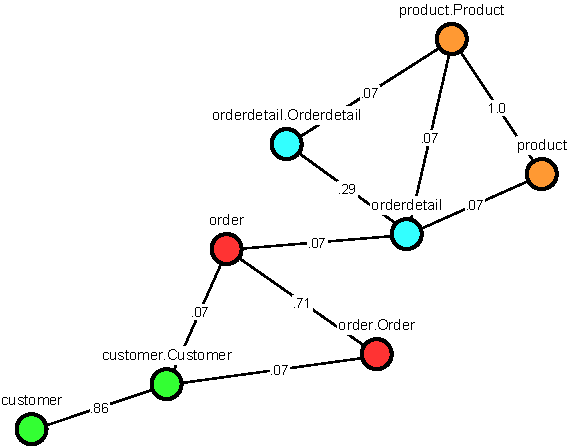
\includegraphics[width=200pt]{figures/data/pypetstore_static_original.pdf}
    \end{subfigure}
    \begin{subfigure}{.5\textwidth}
        \caption{The adjusted PyPetstore version}\label{fig:pypestore_static_swapping_after}
        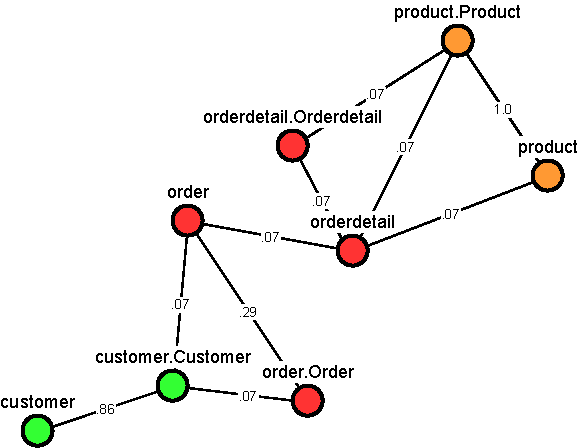
\includegraphics[width=200pt]{figures/data/pypetstore_static_swapped.pdf}
    \end{subfigure}
    \end{adjustbox}
\end{figure}

\begin{figure}[h]
    \caption[The static graph of PyPetstore when manually adding a static dependency.]{The static graph of PyPetstore when an extra call is added from 'order' to 'Product'. The left graph (a) only reflects one call between 'order' and 'Product' while the right graph (b) represents two calls.}
    \label{fig:pypetstore_static_extra_dependencies}
    \begin{adjustbox}{center}
    \begin{subfigure}{.5\textwidth}
        \caption{The adjusted PyPetstore version with one extra dependency.}\label{fig:pypetstore_static_extra_dependencies_1}
        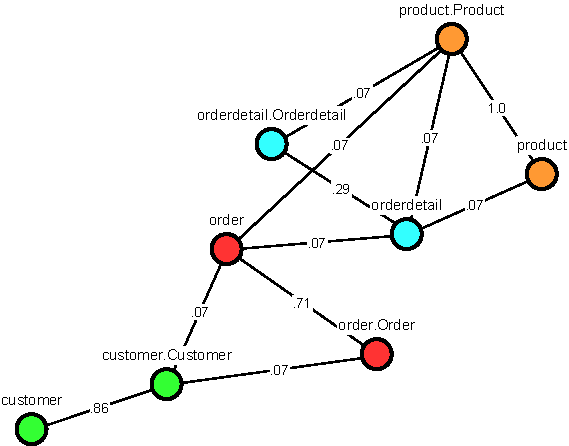
\includegraphics[width=200pt]{figures/data/pypetstore_static_1_added_depend.pdf}
    \end{subfigure}
    \begin{subfigure}{.5\textwidth}
        \caption{The adjusted PyPetstore version with two extra dependencies.}\label{fig:pypetstore_static_extra_dependencies_2}
        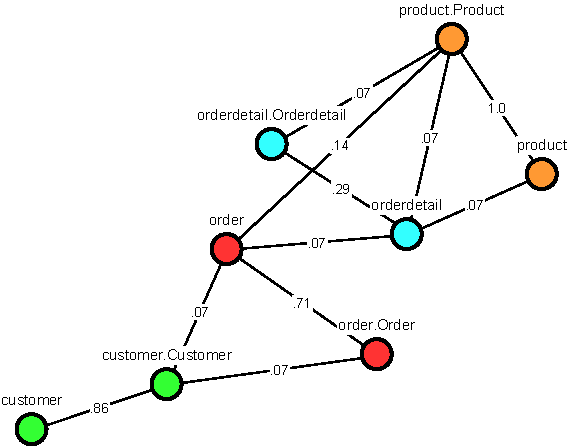
\includegraphics[width=200pt]{figures/data/pypetstore_static_2_added_depend.pdf}
    \end{subfigure}
    \end{adjustbox}
\end{figure}

\paragraph{Adding extra dependencies}
In the second verification test, we adjust the codebase by making a call from the 'order' module to the 'Product' class. The original PyPetstore version does not contain this dependency, and thus we should see a change in the resulting graph. The new decomposition is given in Figure \ref{fig:pypetstore_static_extra_dependencies_1}. When observing this new graph, we notice that indeed a new edge is added between the 'order' module and the 'Product' class. To see how the weight of the edge is determined, we made another variation of PyPetstore where a second call from the 'order' module to the 'Product' graph is added. The resulting graph, shown in Figure \ref{fig:pypetstore_static_extra_dependencies_2}, is similar as before, but the weight between 'order' and 'Product' is increased from a value of 0.7 to 0.14. This is as expected and verifies that the tool works as intended.

\subsection{Verifying semantic dependencies}
The decomposition that results from the original PyPetstore application is given in Figure \ref{fig:pypestore_semantic_before_after}. The figure shows that our tool generates four candidate microservices when only semantic dependencies are included. When comparing it to previous graphs, we see that the semantic graphs contains three additional code fragments, the 'database' module, 'Database' class and the 'main' module. This is possible since code fragments do not necessary need to be invocated by others. The semantic decomposition of the original PyPetstore version is reasonable since we see that semantic related code fragments, such as 'customer' and 'Customer' and 'product' and 'Product', are clustered together. 

\paragraph{Swapping content}
To verify the semantic analyser, we obtain again the decomposition of the adjusted PyPetstore version where the 'Order' and 'Orderdetail' code fragments are swapped. The resulting decomposition appears to be identical to the one in Figure \ref{fig:pypestore_semantic_before_after} and is for this reason not visualised again. This means that swapping code fragments does not influence the result and thus increases the reliability of the tool. \par

\begin{figure}
    \caption[The semantic graph of PyPetstore before and after swapping content.]{The semantic graph of the original and swapped version of PyPetstore. We only show one graph because both appear to be identical.}
    \label{fig:pypestore_semantic_before_after}
    \begin{adjustbox}{center}
    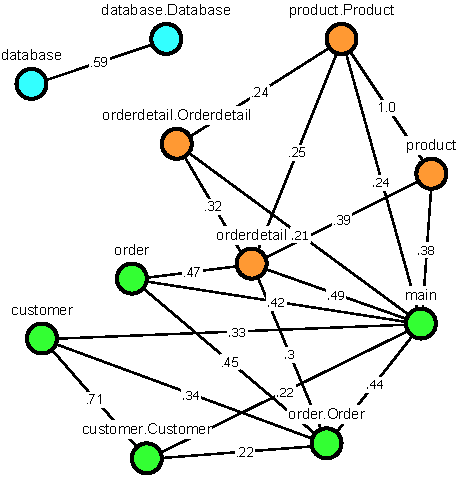
\includegraphics[width=200pt]{figures/data/pypetstore_semantic_original.pdf}
    \end{adjustbox}
\end{figure}

\paragraph{Adding extra terms}
The second test we run is to see how the tool deals with new domain terms. For this reason, we add five times the word 'database' to the 'database' and the 'main' module. With these new terms, we would expect that a new edge arises between the 'main' module and the 'database' module. When observing the new decomposition, we notice that adding the term 'database' does not result in a new semantic dependency. This is because the word database appears very frequently in the program since every module relies on the database. This high term frequency in the program results in a low tf-idf score and therefore does not exceed the threshold value of 0.05. \par
Now, let's try the same, but then with a more discriminate term like 'paper'. Figure \ref{fig:pypetstore_semantic_graph_after_add_terms} shows that indeed a new edge is created now, with a weight of 0.26. This is as expected and thus the test has succeeded.

\begin{figure}
    \caption{The semantic graph of PyPetstore after adding the term 'paper' five times in 'main' and 'database'.}
    \label{fig:pypetstore_semantic_graph_after_add_terms}
    \begin{adjustbox}{center}
    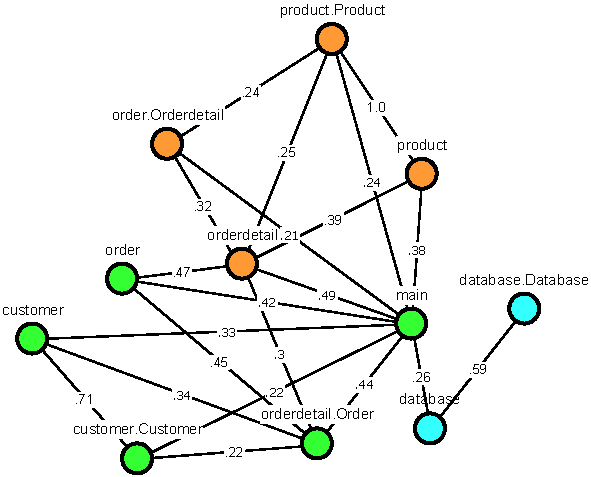
\includegraphics[width=300pt]{figures/data/pypetstore_semantic_add_depend.pdf}
    \end{adjustbox}
\end{figure}

\subsection{Verifying dynamic dependencies}
The decomposition of the original PyPetstore version constructed with dynamic dependencies is given in Figure \ref{fig:pypestore_dynamic_before}. The dynamic decomposition results in four services and is the only decomposition that also included the 'util' module. 

\paragraph{Swapping content}
Also for the dynamic dependency graph, we verify how it copes with code fragments that are swapped. Important for this test is that both the manipulated and the original PyPetstore versions are ran on the same test scenarios. This way, they both have the same logs and thus should make the same decomposition. The results, given in Figure \ref{fig:pypestore_dynamic_before}, show that both decompositions are identical. Since both decompositions are identical, we only visualised one in Figure \ref{fig:pypestore_dynamic_before}.

\paragraph{Adding extra test scenarios}
For the last verification test, we give the adjusted PyPetstore version two times the log files. This means that the expected outcome would be the exact same decomposition. This is because the strength of the edges are normalised, and thus a higher frequency cannot be seen from the graph. The result decomposition when adding twice the log files are identical to the one given in Figure \ref{fig:pypestore_dynamic_before}.

\begin{figure}
    \caption[The dynamic graph of PyPetstore.]{The dynamic graph of the original and swapped version of PyPetstore. We only show one graph because both appear to be identical.}
    \label{fig:pypestore_dynamic_before}
    \begin{adjustbox}{center}
    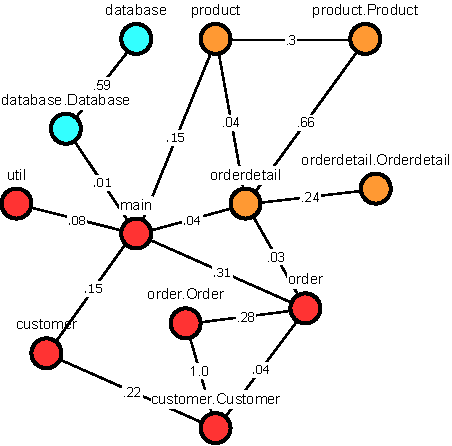
\includegraphics[width=200pt]{figures/data/pypetstore_dynamic_original.pdf}
    \end{adjustbox}
\end{figure}


\chapter{Evaluation}\label{c:results}\label{c:results}
This chapter presents the results of the main experiment and is structured as follows. At first, we describe the design of the experiment. This is done by discussing the different groups that are tested against each other, the algorithm that is used to obtain the decomposition, and the input projects used for experimentation. After the experimental design, we present the results of the experiment. 

\section{Experimental design}
To understand the effect of the utilised information stream on the microservice decomposition, we make seven different decompositions of the system with our proposed tool. Each decomposition is constructed with a unique stream of data. The different input data streams are listed below. Each input stream gets an identifier of three letters based on the data it incorporates. The first letter $S$ represents static data, the second one $L$ lexical data, and the third one $D$ dynamic data. When a data source is not included, the letter $X$ is given.

\begin{itemize}
    \item[$SXX$] \textbf{Static.} The candidate microservices that are obtained by only considering static dependencies as input.
    \item[$XLX$] \textbf{Lexical.} The decompositions obtained when only considering semantic information. This means the graph only consists of semantic edges.
    \item[$XXD$] \textbf{Dynamic.} The decompositions constructed with only dynamic dependencies.
    \item[$SXD$] \textbf{Static and dynamic.} These decompositions are constructed with static and dynamic data as input. This means that both the static and dynamic edges are given in the graph. When an edge has both a static and a dynamic dependency, the edge weights are combined by taking 50 percent of each weight.
    \item[$SLX$] \textbf{Static and semantic.} The fifth group of decompositions combines static with semantic information as input. The edges are combined the same way as before.
    \item[$XLD$] \textbf{Dynamic and semantic.} These decompositions are constructed with dynamic and semantic information as input.
    \item[$SLD$] \textbf{Static, dynamic and semantic.} This group of decompositions takes all three streams of data as input. This means, the edges in the graph can either represent a static, semantic or dynamic edge, or a combination of those. When an edge is combined, each information source counts for 33 percent. This way the maximum weight of the combined edge can never exceed a value of 1. 
\end{itemize}

\subsection{Algorithm and parameters}
The aim of this thesis is the understand how the quality of the microservices changes when different streams of data are used. To make sure the change in the quality of the decomposition is caused by the selected stream of data, it is important to understand how the clustering algorithm influences the result. In the next section, we therefore analyse the impact of the clustering algorithm on the quality of the resulting decomposition.

\subsubsection{The effect of the clustering algorithm}
To measure the effect of the clustering algorithm, we apply the three clustering algorithms selected in Section \ref{step3:graphs} on three graphs created with static, semantic and the two combined as input. Since the Clauset-Newman-Moore algorithm gave strange results for the CHM and CHD metric, we incorporated a fourth clustering algorithm called Label Propogation. The Label Propogation algorithm (LPA), introduced by \citeauthor{raghavan2007near} \cite{raghavan2007near}, is hierarchical based and has an agglomerative character.\par
The three graphs are constructed for two monolithic projects of different sizes. We then observe the change in the results in terms of CHD, CHM, SMQ, and CMQ. When the change in the results are the same direction (all positive or negative) for each clustering algorithm, we assume the algorithm does not affect the change of the results. The results of this experiment are given in Table \ref{tab:effect_algorithm}. \par

\begin{table}[h]
    \footnotesize
    \caption[The effect of the clustering algorithm.]{Results on the effect of the clustering algorithm.}\label{tab:effect_algorithm}
    %This table gives the results of four clustering algorithms applied on three experiments. The best results for Louvain were found with a resolution value of 1. Girvan-Newman gave the best resolution with a cutting value of 5. The last row shows the most frequent change in the results when comparing it to previous column. $>$ indicates the value of the former is bigger than the latter and $<$ vice versa. The number in the brackets shows how many times the change happens. When the change is equal, the $=$ symbol is used. 
    \begin{adjustbox}{center}
    \begin{tabular}{>{\raggedright}m{20pt}>{\raggedright}m{75pt}>{\raggedright}m{18pt}>{\raggedright}m{18pt}>{\raggedright}m{18pt}>{\raggedright}m{18pt}>{\raggedright}m{18pt}>{\raggedright}m{18pt}>{\raggedright}m{18pt}>{\raggedright}m{18pt}>{\raggedright}m{18pt}>{\raggedright}m{18pt}>{\raggedright}m{18pt}>{\raggedright\arraybackslash}m{18pt}}
        \toprule
        Mono
        & Algo
        & \multicolumn{3}{c}{CHM} 
        & \multicolumn{3}{c}{CHD}
        & \multicolumn{3}{c}{SMQ}
        & \multicolumn{3}{c}{CMQ} \\
        & & $SXX$ & $XLX$ & $SLX$ & $SXX$ & $XLX$ & $SLX$ & $SXX$ & $XLX$ & $SLX$ & $SXX$ & $XLX$ & $SLX$ \\
        \midrule
        \multirow{4}*{$M_2$} & Louvain & 0.667 & 0.609 & 0.750 & 0.701 & 0.742 & 0.813 & 0.124 & 0.033 & 0.048 & 0.060 & 0.226 & 0.137 \\
        & Girvan-Newman & 0.498 & 0.586 & 0.619 & 0.562 & 0.753 & 0.754 & 0.092 & 0.021 & 0.012 & 0.039 & 0.199 & 0.197 \\
        & Clauset & 0.440 & 0 & 0 & 0.519 & 0 & 0 & 0.090 & 0.009 & 0.019 & 0.033 & 0.050 & 0.043 \\
        & LPA & 0.667 & 0.620 & 0.657 & 0.695 & 0.745 & 0.783 & 0.170 & 0.039 & 0.056 & 0.081 & 0.254 & 0.188 \\
        \midrule
        \midrule
        & Change & - & (3)$>$ & (3)$<$ & - & (3)$<$ & (3)$<$ & - & (4)$>$ & (4)$<$ & - & (4)$<$ & (4)$>$ \\
        \midrule
        \multirow{4}*{$M_4$} & Louvain & 0.762 & 0.600 & 0.661 & 0.792 & 0.665 & 0.708 & 0.180 & 0.032 & 0.039 & 0.160 & 0.225 & 0.221 \\
        & Girvan-Newman & 0.619 & 0.788 & 0.812 & 0.613 & 0.846 & 0.886 & 0.160 & 0.015 & 0.010 & 0.148 & 0.266 & 0.199 \\
        & Clauset & 1 & 0 & 0 & 1 & 0 & 0 & 0.204 & 0.009 & 0.012 & 0.202 & 0.083 & 0.079 \\
        & LPA & 0.799 & 0.712 & 0.814 & 0.792 & 0.733 & 0.798 & 0.211 & 0.069 & 0.076 & 0.162 & 0.232 & 0.228 \\
        \midrule
        \midrule
        & Change & - & (3)$>$ & (3)$<$ & - & (3)$>$ & (3)$<$ & - & (4)$>$ & (3)$<$ & - & (3)$<$ & (4)$>$ \\
        \bottomrule
    \end{tabular}
    \end{adjustbox}
\end{table}

The Louvain algorithm is tested with different resolution parameters ranging between the values 0.3 and 1. The resolution value with the best performance is chosen and given in the table. The same applies for the input parameter for the Girvan-Newman algorithm. We tried different cutting values ranging between 0 and 5 and selected the best performing one. \par
The row under the double line shows the most frequent type of change that occurs in the results when comparing it to previous column. The greater than ($>$) symbol indicates that the value of the former is bigger than the latter and the less than ($<$) symbol the opposite. The number in the brackets shows how many times the change happens. When the change is equal, the $=$ symbol is used. \par
The table above (Table \ref{tab:effect_algorithm}) shows that most of the times the change in the results is the same for the algorithms. From the 106 observed changes, 96 appear to have the same direction. This means that 91 percent of the changes are the same regardless of the clustering algorithm. For this reason, we decided to select only one algorithm for the main experiment. We decided to go for the Louvain algorithm with a resolution parameter of 1, as it gave the most satisfying and consistent results. For the tf-idf threshold value, we selected a value of 0.05. Increasing this value results in a lower coverage of the semantic constructed graph. A value of 0.05 gave satisfying results during verification and will therefore be used in the remaining experiment.

\subsection{Project collection}
Table \ref{tab:projects_statistics} shows the projects that are used for experimentation. Each monolithic project $M$ is enriched with some descriptive statistics, such as the source lines of code (SLOC) and the number of classes, modules, methods and functions. Below, we give a short description of each project. The projects are ordered by its complexity (in terms of SLOC), starting with the smallest project.

\begin{enumerate}
    \item[$M_1$]\textbf{PyPystore.} PyPetstore\footnote{\href{https://github.com/larsvasseldonk/PyPetstore}{https://github.com/larsvasseldonk/PyPetstore}} is a minimal working command-line tool, inspired by JPetstore, that supports the process of selling pets. PyPetstore serves as an 'toy' example in which we can verify the working of our proposed technique.
    \item[$M_2$] \textbf{twitter} The twitter\footnote{\href{https://github.com/python-twitter-tools/twitter}{https://github.com/python-twitter-tools/twitter}} project includes a set of Python tools such as a Twitter API, command-line tool, and IRC bot. The command-line tool allows you to, e.g., get friends' tweets and setting your own tweet. The IRC bot announces Twitter updates to an IRC channel. 
    \item[$M_3$] \textbf{ChatterBot.} ChatterBot\footnote{\href{https://github.com/gunthercox/ChatterBot}{https://github.com/gunthercox/ChatterBot}} is a machine-learning based conversational dialog engine build in Python which makes it possible to generate responses based on collections of known conversations.
    \item[$M_4$] \textbf{asreview.} ASReview\footnote{\href{https://github.com/asreview/asreview}{https://github.com/asreview/asreview}} (Active learning for Systematic Reviews) implements machine learning algorithms that interactively query the researcher. The project is developed and maintained by Utrecht University and is designed to accelerate the step of screening abstracts and titles with a minimum of papers to be read by a human.
    \item[$M_5$] \textbf{beets.} Beets\footnote{\href{https://github.com/beetbox/beets}{https://github.com/beetbox/beets}} is the media library management system for obsessive music geeks. The project enables users manage music collections by, e.g., automatically improving metadata. It also provides a set of tools to manipulate and access music.
    \item[$M_6$] \textbf{Picard.} MusicBrainz Picard\footnote{\href{https://github.com/metabrainz/picard}{https://github.com/metabrainz/picard}} is a cross-platform (Linux/Mac OS X/Windows) application written in Python and is the official MusicBrainz tagger. The project's public facing website is \href{https://picard.musicbrainz.org/}{https://picard.musicbrainz.org/}. MusicBrainz is an open music encyclopedia that collects music metadata and makes it available to the public.
    \item[$M_7$] \textbf{mu.} Mu\footnote{\href{https://github.com/mu-editor/mu}{https://github.com/mu-editor/mu}} is a simple code editor for beginner programmers based on extensive feedback from teachers and learners. The project's public facing website is \href{https://codewith.mu/}{https://codewith.mu/}.
\end{enumerate}

\begin{table}[h]
    \small
    \caption[Python project for experimentation]{Python projects for experimentation. For each project, we have collected the number of modules, classes, methods and functions available in the code base. The SLOC resembles the number of Python lines of code. }\label{tab:projects_statistics}
    \begin{tabular}{>{\raggedright}m{60pt}>{\raggedright}m{35pt}>{\raggedright}m{30pt}>{\raggedright}m{35pt}>{\raggedright}m{40pt}>{\raggedright\arraybackslash}m{50pt}}
        \toprule
        Project & SLOC & Files & Classes & Methods & Functions\\
        \midrule
        PyPetstore & 556 & 8 & 5 & 40 & 18\\
        \midrule
        twitter & 3510 & 17 & 66 & 117 & 64 \\
        \midrule
        Chatterbot & 10297 & 39 & 46 & 124 & 30 \\
        \midrule
        asreview & 11947 & 101 & 58 & 256 & 280 \\
        \midrule
        beets & 44829 & 29 & 134 & 575 & 290 \\
        \midrule
        picard & 62559 & 196 & 352 & 2027 & 465 \\
        \midrule
        mu & 78628 & 45 & 71 & 524 & 70 \\
        \bottomrule
    \end{tabular}  
\end{table}

\section{Results}
Each of the aforementioned project is analysed with our multi-view clustering tool. Out of this tool, a set of static, semantic and dynamic edges derives. These edges are then used to construct seven different graphs. Subsequently, the Louvain algorithm is used to find communities (microservices) in the graph such that nodes within a community are highly connected, and nodes between communities have low connections. The nodes in the graph represent top-level code fragments, where each top-level code fragment can either be a module (with its inner functions) or a class (with its inner methods). The quality of the candidate micoservices are then measured with the functional independence and modularity metrics. To understand what the effect of the input data is, we rigorously test if the quality of a decomposition resulting from a given information stream outperforms another. We use the paired t-test to validate whether the quality of two decomposition made with different streams of information are significantly different. Two groups are significantly different when the paired t-test results in a p-value lower than 0.05. In the next sections, we give the results of the experiment for each quality metric. \par

\subsection{Functional independence}
As described in Section \ref{s:quality_computation}, we measure the quality of the resulting candidate microservices in terms of its functional independence. The functional independence is measured according to four metrics, namely, CHD, CHM, IFN and OPN. Table \ref{tab:results_chd}, \ref{tab:results_chm}, \ref{tab:results_ifn}, and \ref{tab:results_opn} show the result of each metric respectively when applying our tool with different input data. The last row of each table gives the mean value of each experiment. The experiment with the best mean score is marked with a grey cell colour.

\paragraph{Cohesion at domain level} The CHD metrics aims to measure the cohesiveness of services at domain level. The higher the CHD, the more functional cohesive the services are \cite{jin2018functionality}. Table \ref{tab:results_chd} shows the CHD scores for each input information stream. On average, the highest score for CHD is achieved when all three information streams are used for the decomposition ($SLD$). This makes sense since the algorithm has more information to make a suitable decomposition. However, it is not always that more information results in higher CHD scores. When static and dynamic is combined as input ($SXD$), the average CHD score lies somewhere between the two CHD scores achieved when both streams are used individually ($SXX$ and $XXD$). However, this is on average. When we look at the data again, we note that bigger applications ($M_5$, $M_6$, and $M_7$) always get a higher CHD score when static and dynamic data are combined as input than when they are used individually. The same pattern applies when static and lexical data streams ($SLX$) are combined as input. On average, this again results in a higher CHD score (0.615) than when only static (0.544) or only lexical (0.598) are used. This pattern is in line with our expectations that more views of the system result in a higher quality of the decomposition. When lexical and dynamic information ($XLD$) are combined as input, we see a small decrease in the average CHD score (0.591) compared to the average CHD score achieved when lexical data ($XLX$) is used only (0.598). However, the score is still higher than only using dynamic information ($XXD$) as input (0.537). Each combination of input streams is tested with a paired t-test, but none of them are significantly different. 

\begin{table}[h]
    \footnotesize
    \caption{Results of the main experiment in terms of CHD.}\label{tab:results_chd}
    \begin{adjustbox}{center}
    \begin{tabular}{>{\raggedright}m{20pt}>{\raggedright}m{20pt}>{\raggedright}m{25pt}>{\raggedright}m{20pt}>{\raggedright}m{20pt}>{\raggedright}m{25pt}>{\raggedright}m{20pt}>{\raggedright\arraybackslash}m{20pt}}
        \toprule
        Mono
        & \multicolumn{7}{c}{CHD}\\
        & $SXX$ & $XLX$ & $XXD$ & $SXD$ & $SLX$ & $XLD$ & $SLD$\\
        \midrule
        $M_1$ 
        & 0.511 & 0.479 & 0.528 & 0.479 & 0.417 & 0.479 & 0.479\\
        $M_2$ 
        & 0.375 & 0.641 & 0.633 & 0.375 & 0.595 & 0.624 & 0.632 \\
        $M_3$ 
        & 0.500 & 0.494 & 0.567 & 0.457 & 0.557 & 0.562 & 0.485 \\
        $M_4$ 
        & 0.755 & 0.688 & 0.579 & 0.655 & 0.693 & 0.681 & 0.706 \\
        $M_5$ 
        & 0.452 & 0.496 & 0.336 & 0.506 & 0.506 & 0.451 & 0.509 \\
        $M_6$ 
        & 0.770 & 0.746 & 0.631 & 0.810 & 0.748 & 0.734 & 0.771 \\
        $M_7$ 
        & 0.448 & 0.642 & 0.484 & 0.501 & 0.791 & 0.605 & 0.786 \\
        \midrule
        \midrule
        $avg$ & 0.544 & 0.598 & 0.537 & 0.540 & 0.615 & 0.591 & \cellcolor{CellGray}0.624\\
        \bottomrule
    \end{tabular}
    \end{adjustbox}
\end{table}

% Projects are alphabetically ordered
% IN: IN1 & IN2 & IN3 & IN4 & IN5 & IN6 & IN7

% M1 PyPetstore
% CHM: 0.756 & 0.305 & 0.369 & 0.250 & 0.667 & 0.250 & 0.250
% CHD: 0.511 & 0.044 & 0.528 & 0.479 & 0.444 & 0.479 & 0.479
% IFN: 1.25 & 4 & 2 & 1.333 & 1 & 1.333 & 1.333
% OPN: 15 & 18 & 19 & 10 & 7 & 10 & 10
% SMQ: 0.125 & -0.094 & 0.167 & 0.211 & 0.146 & 0.211 & 0.211
% CMQ: 0.125 & 0.062 & 0.086 & 0.127 & -0.042 & 0.125 & 0.125
% CF: 0.655 & 0.793 & 0.653 & 0.947 & 0.773 & 0.838 & 0.88
% Coverage: 0.667 & 0.667 & 1 & 0.667 & 1 & 1

% M2 twitter
% CHM: 0.293 & 0.721 & 0.704 & 0.486 & 0.755 & 0.772 & 0.766
% CHD: 0.5 & 0.661 & 0.667 & 0.636 & 0.789 & 0.745 & 0.773
% IFN: 2 & 3.625 & 4.5 & 3.667 & 2.714 & 3.875 & 3.667
% OPN: 20 & 53 & 16 & 26 & 32 & 49 & 37
% SMQ: 0.149 & 0.022 & 0.11 & 0.142 & 0.052 & 0.041 & 0.052
% CMQ: 0.114 & 0.198 & 0.077 & 0.09 & 0.176 & 0.207 & 0.146
% CF: 0.684 & 0.774 & 0.628 & 0.561 & 0.744 & 0.881 & 0.871
% Coverage: 0.615 & 0.910 & 0.423 & 0.756 & 0.962 & 0.987 & 0.987

% M3 ChatterBot
% CHM: 0.752 & 0.516 & 0.673 & 0.563 & 0.568 & 0.489 & 0.561
% CHD: 0.767 & 0.409 & 0.517 & 0.463 & 0.529 & 0.408 & 0.513
% IFN: 2.5 & 4 & 2.25 & 2.857 & 3.5 & 4.6 & 4
% OPN: 28 & 46 & 20 & 43 & 48 & 58 & 42
% SMQ: 0.190 & 0.030 & 0.138 & 0.149 & 0.069 & 0.038 & 0.050
% CMQ: 0.044 & 0.233 & 0.030 & 0.027 & 0.126 & 0.136 & 0.108
% Coverage: 0.449 & 0.878 & 0.653 & 0.714 & 0.898 & 0.959 & 0.980

% M4 asreview
% CHM: 0.747 & 0.668 & 0.696 & 0.707 & 0.725 & 0.669 & 0.661
% CHD: 0.730 & 0.612 & 0.599 & 0.665 & 0.685 & 0.627 & 0.630
% IFN: 4.5 & 9.6 & 4.833 & 4.125 & 7.8 & 8.333 & 8.8
% OPN: 55 & 112 & 73 & 81 & 80 & 113 & 90
% SMQ: 0.179 & 0.033 & 0.175 & 0.192 & 0.038 & 0.034 & 0.039
% CMQ: 0.169 & 0.224 & 0.054 & 0.133 & 0.223 & 0.203 & 0.15
% Coverage: 0.732 & 0.961 & 0.661 & 0.913 & 0.984 & 0.992 & 1

% M5 beets
% CHM: 0.627 & 0.653 & 0.570 & 0.604 & 0.649 & 0.644 & 0.622
% CHD: 0.365 & 0.527 & 0.450 & 0.510 & 0.528 & 0.514 & 0.481
% IFN: 4.667 & 14.8 & 7.167 & 6.667 & 12.667 & 14.4 & 12.167
% OPN: 100 & 234 & 162 & 127 & 238 & 215 & 225
% SMQ: 0.152 & 0.02 & 0.082 & 0.128 & 0.022 & 0.023 & 0.03
% CMQ: 0.141 & 0.165 & 0.045 & 0.106 & 0.173 & 0.167 & 0.167
% Coverage: 0.645 & 1 & 0.671 & 0.865 & 1 & 1 & 1

% M6 picard
% CHM: 0.799 & 0.712 & 0.667 & 0.799 & 0.690 & 0.735 & 0.759
% CHD: 0.871 & 0.784 & 0.757 & 0.851 & 0.759 & 0.812 & 0.806
% IFN: 4.688 & 23.5 & 3.667 & 5.933 & 21.25 & 26 & 18.5
% OPN: 112 & 357 & 109 & 138 & 321 & 332 & 267
% SMQ: 0.139 & 0.009 & 0.153 & 0.130 & 0.016 & 0.008 & 0.024
% CMQ: 0.133 & 0.155 & 0.114 & 0.113 & 0.143 & 0.146 & 0.160
% Coverage: 0.69 & 0.998 & 0.4 & 0.841 & 1 & 0.998 & 1

% M7 mu
% CHM: 0.720 & 0.699 & 0.537 & 0.802 & 0.737 & 0.739 & 0.782
% CHD: 0.472 & 0.564 & 0.359 & 0.584 & 0.517 & 0.624 & 0.546
% IFN: 2.143 & 8.8 & 2.4 & 2.556 & 4.4 & 6.667 & 3.8
% OPN: 44 & 121 & 30 & 58 & 55 & 87 & 48
% SMQ: 0.154 & 0.021 & 0.132 & 0.157 & 0.084 & 0.036 & 0.085
% CMQ: 0.115 & 0.119 & 0.032 & 0.097 & 0.110 & 0.124 & 0.111
% Coverage: 0.733 & 0.933 & 0.544 & 0.833 & 0.944 & 0.989 & 1


% Data per group (experiment) for statistical test

% PICARD NOT YET INCLUDED
% CHD
% ex1: 0.511, 0.500, 0.767, 0.730, 0.365, 0.871, 0.472
% ex2: 0.044, 0.661, 0.409, 0.612, 0.527, 0.784, 0.564
% ex3: 0.528, 0.667, 0.517, 0.599, 0.450, 0.757, 0.359
% ex4: 0.479, 0.636, 0.463, 0.665, 0.510, 0.851, 0.584
% ex5: 0.444, 0.789, 0.529, 0.685, 0.528, 0.759, 0.517
% ex6: 0.479, 0.745, 0.408, 0.627, 0.514, 0.812, 0.624
% ex7: 0.479, 0.773, 0.513, 0.630, 0.481, 0.806, 0.546

% CHM
% ex1: 0.756, 0.293, 0.752, 0.747, 0.627, 0.799, 0.720
% ex2: 0.305, 0.721, 0.516, 0.668, 0.653, 0.712, 0.699
% ex3: 0.369, 0.704, 0.673, 0.696, 0.570, 0.667, 0.537
% ex4: 0.250, 0.486, 0.563, 0.707, 0.604, 0.799, 0.802
% ex5: 0.667, 0.755, 0.568, 0.725, 0.649, 0.690, 0.737
% ex6: 0.250, 0.772, 0.489, 0.669, 0.644, 0.735, 0.739
% ex7: 0.250, 0.766, 0.561, 0.661, 0.622, 0.759, 0.782

% IFN
% ex1: 1.25, 2, 2.5, 4.5, 4.667, 4.688, 2.143
% ex2: 4, 3.625, 4, 9.6, 14.8, 23.5, 8.8
% ex3: 2, 4.5, 2.25, 4.833, 7.167, 3.667, 2.4
% ex4: 1.333, 3.667, 2.857, 4.125, 6.667, 5.933, 2.556
% ex5: 1, 2.714, 3.5, 7.8, 12.667, 21.25, 4.4
% ex6: 1.333, 3.875, 4.6, 8.333, 14.4, 26, 6.667
% ex7: 1.333, 3.667, 4, 8.8, 12.167, 18.5, 3.8

% OPN
% ex1: 15, 20, 28, 55, 100, 112, 44
% ex2: 18, 53, 46, 112, 234, 357, 121
% ex3: 19, 16, 20, 73, 162, 109, 30
% ex4: 10, 26, 43, 81, 127, 138, 58
% ex5: 7, 32, 48, 80, 238, 321, 55
% ex6: 10, 49, 58, 113, 215, 332, 87
% ex7: 10, 37, 42, 90, 225, 267, 48

% SMQ
% ex1: 0.125, 0.149, 0.190, 0.179, 0.152, 0.139, 0.154
% ex2: -0.094, 0.022, 0.030, 0.033, 0.020, 0.009, 0.021
% ex3: 0.167, 0.11, 0.138, 0.175, 0.082, 0.153, 0.132
% ex4: 0.211, 0.142, 0.149, 0.192, 0.128, 0.130, 0.157
% ex5: 0.146, 0.052, 0.069, 0.038, 0.022, 0.016, 0.084
% ex6: 0.211, 0.041, 0.038, 0.034, 0.023, 0.008, 0.036
% ex7: 0.211, 0.052, 0.050, 0.039, 0.03, 0.024, 0.085

% CMQ:
% ex1: 0.125, 0.114, 0.044, 0.169, 0.141, 0.133, 0.115
% ex2: 0.062, 0.198, 0.233, 0.224, 0.165, 0.155, 0.119
% ex3: 0.086, 0.077, 0.030, 0.054, 0.045, 0.114, 0.032
% ex4: 0.127, 0.090, 0.027, 0.133, 0.106, 0.113, 0.097
% ex5: -0.042, 0.176, 0.126, 0.233, 0.173, 0.143, 0.110
% ex6: 0.125, 0.207, 0.136, 0.203, 0.167, 0.146, 0.124
% ex7: 0.125, 0.146, 0.108, 0.15, 0.167, 0.160, 0.111

% Coverage
% ex1: 0.667, 0.615, 0.449, 0.732, 0.645, 0.690, 0.733
% ex2: 0.667, 0.910, 0.878, 0.961, 1, 0.998, 0.993
% ex3: 1, 0.423, 0.653, 0.661, 0.671, 0.4, 0.544
% ex4: 1, 0.756, 0.714, 0.913, 0.865, 0.841, 0.833
% ex5: 0.667, 0.962, 0.898, 0.984, 1, 1, 0.944
% ex6: 1, 0.987, 0.959, 0.992, 1, 0.998, 0.989
% ex7: 1, 0.987, 0.980, 1, 1, 1, 1

\paragraph{Cohesion at message level}
The cohesion at message level (CHM) metric, explained in Section \ref{sss:step4_chm}, measures how cohesive services are based on the similarity of the input and output parameters of the operations in a service that communicate with other services. A higher score for CHM means a more cohesive decomposition and is preferred. Table \ref{tab:results_chm} gives the CHM results of the main experiment. The highest average CHM value is reached when static and lexical ($SLX$) information are combined as input (0.663). When also dynamic information is included ($SLD$), the CHM slightly decreases to a value of 0.643. However, the score of $SLD$ is for all projects at least as good as the worst performing individual score. For the bigger projects $M_5$, $M_6$ and $M_7$, the CHM score always outperforms two individual streams of data.
Another pattern that we observe in the CHM results is that on average the CHM value increases when static ($SXX$) and dynamic graphs ($XXD$) are supplemented with semantic data ($SLX$ and $XLD$). Moreover, we see that combining static and dynamic ($SXD$) data streams does not result in an increase in score when comparing it to their individual scores. On average, the result of $SXD$ (0.574) appears to be lower than the two individual scores of $SXX$ (0.643) and $XXD$ (0.578). The changes in the score are small and after running the statistical tests it appears that there is not a significant difference between them.

\begin{table}[h]
    \footnotesize
    \caption{Results of the main experiment in terms of CHM.}\label{tab:results_chm}
    \begin{adjustbox}{center}
    \begin{tabular}{>{\raggedright}m{20pt}>{\raggedright}m{20pt}>{\raggedright}m{25pt}>{\raggedright}m{20pt}>{\raggedright}m{20pt}>{\raggedright}m{25pt}>{\raggedright}m{20pt}>{\raggedright\arraybackslash}m{20pt}}
        \toprule
        Mono
        & \multicolumn{7}{c}{CHM}\\
        & $SXX$ & $XLX$ & $XXD$ & $SXD$ & $SLX$ & $XLD$ & $SLD$\\
        \midrule
        $M_1$ 
        & 0.756 & 0.250 & 0.369 & 0.250 & 0.333 & 0.250 & 0.250\\
        $M_2$ 
        & 0.189 & 0.700 & 0.428 & 0.189 & 0.592 & 0.638 & 0.567 \\
        $M_3$ 
        & 0.524 & 0.531 & 0.724 & 0.586 & 0.579 & 0.579 & 0.529\\
        $M_4$ 
        & 0.792 & 0.770 & 0.658 & 0.703 & 0.732 & 0.765 & 0.754 \\
        $M_5$ 
        & 0.683 & 0.669 & 0.562 & 0.657 & 0.701 & 0.621 & 0.691 \\
        $M_6$ 
        & 0.858 & 0.794 & 0.722 & 0.873 & 0.798 & 0.795 & 0.810 \\
        $M_7$ 
        & 0.696 & 0.803 & 0.645 & 0.758 & 0.898 & 0.733 & 0.899 \\
        \midrule
        \midrule
        $avg$ & 0.643 & 0.645 & 0.587 & 0.574 & \cellcolor{CellGray}0.662 & 0.626 & 0.643\\
        \bottomrule
    \end{tabular}
    \end{adjustbox}
\end{table}

% Projects are alphabetically ordered
% IN: IN1 & IN2 & IN3 & IN4 & IN5 & IN6 & IN7

% M1 PyPetstore
% CHM: 0.756 & 0.305 & 0.369 & 0.250 & 0.667 & 0.250 & 0.250
% CHD: 0.511 & 0.044 & 0.528 & 0.479 & 0.444 & 0.479 & 0.479
% IFN: 1.25 & 4 & 2 & 1.333 & 1 & 1.333 & 1.333
% OPN: 15 & 18 & 19 & 10 & 7 & 10 & 10
% SMQ: 0.125 & -0.094 & 0.167 & 0.211 & 0.146 & 0.211 & 0.211
% CMQ: 0.125 & 0.062 & 0.086 & 0.127 & -0.042 & 0.125 & 0.125
% CF: 0.655 & 0.793 & 0.653 & 0.947 & 0.773 & 0.838 & 0.88
% Coverage: 0.667 & 0.667 & 1 & 0.667 & 1 & 1

% M2 twitter
% CHM: 0.293 & 0.721 & 0.704 & 0.486 & 0.755 & 0.772 & 0.766
% CHD: 0.5 & 0.661 & 0.667 & 0.636 & 0.789 & 0.745 & 0.773
% IFN: 2 & 3.625 & 4.5 & 3.667 & 2.714 & 3.875 & 3.667
% OPN: 20 & 53 & 16 & 26 & 32 & 49 & 37
% SMQ: 0.149 & 0.022 & 0.11 & 0.142 & 0.052 & 0.041 & 0.052
% CMQ: 0.114 & 0.198 & 0.077 & 0.09 & 0.176 & 0.207 & 0.146
% CF: 0.684 & 0.774 & 0.628 & 0.561 & 0.744 & 0.881 & 0.871
% Coverage: 0.615 & 0.910 & 0.423 & 0.756 & 0.962 & 0.987 & 0.987

% M3 ChatterBot
% CHM: 0.752 & 0.516 & 0.673 & 0.563 & 0.568 & 0.489 & 0.561
% CHD: 0.767 & 0.409 & 0.517 & 0.463 & 0.529 & 0.408 & 0.513
% IFN: 2.5 & 4 & 2.25 & 2.857 & 3.5 & 4.6 & 4
% OPN: 28 & 46 & 20 & 43 & 48 & 58 & 42
% SMQ: 0.190 & 0.030 & 0.138 & 0.149 & 0.069 & 0.038 & 0.050
% CMQ: 0.044 & 0.233 & 0.030 & 0.027 & 0.126 & 0.136 & 0.108
% Coverage: 0.449 & 0.878 & 0.653 & 0.714 & 0.898 & 0.959 & 0.980

% M4 asreview
% CHM: 0.747 & 0.668 & 0.696 & 0.707 & 0.725 & 0.669 & 0.661
% CHD: 0.730 & 0.612 & 0.599 & 0.665 & 0.685 & 0.627 & 0.630
% IFN: 4.5 & 9.6 & 4.833 & 4.125 & 7.8 & 8.333 & 8.8
% OPN: 55 & 112 & 73 & 81 & 80 & 113 & 90
% SMQ: 0.179 & 0.033 & 0.175 & 0.192 & 0.038 & 0.034 & 0.039
% CMQ: 0.169 & 0.224 & 0.054 & 0.133 & 0.223 & 0.203 & 0.15
% Coverage: 0.732 & 0.961 & 0.661 & 0.913 & 0.984 & 0.992 & 1

% M5 beets
% CHM: 0.627 & 0.653 & 0.570 & 0.604 & 0.649 & 0.644 & 0.622
% CHD: 0.365 & 0.527 & 0.450 & 0.510 & 0.528 & 0.514 & 0.481
% IFN: 4.667 & 14.8 & 7.167 & 6.667 & 12.667 & 14.4 & 12.167
% OPN: 100 & 234 & 162 & 127 & 238 & 215 & 225
% SMQ: 0.152 & 0.02 & 0.082 & 0.128 & 0.022 & 0.023 & 0.03
% CMQ: 0.141 & 0.165 & 0.045 & 0.106 & 0.173 & 0.167 & 0.167
% Coverage: 0.645 & 1 & 0.671 & 0.865 & 1 & 1 & 1

% M6 picard

% M7 mu
% CHM: 0.720 & 0.699 & 0.537 & 0.802 & 0.737 & 0.739 & 0.782
% CHD: 0.472 & 0.564 & 0.359 & 0.584 & 0.517 & 0.624 & 0.546
% IFN: 2.143 & 8.8 & 2.4 & 2.556 & 4.4 & 6.667 & 3.8
% OPN: 44 & 121 & 30 & 58 & 55 & 87 & 48
% SMQ: 0.154 & 0.021 & 0.132 & 0.157 & 0.084 & 0.036 & 0.085
% CMQ: 0.115 & 0.119 & 0.032 & 0.097 & 0.110 & 0.124 & 0.111
% Coverage: 0.733 & 0.933 & 0.544 & 0.833 & 0.944 & 0.989 & 1

\paragraph{Number of interfaces}
The third metric to measure how functional independent the decomposition is, is the average number of interfaces a service provides. The aim is to get the lowest IFN rate as possible. Table \ref{tab:results_ifn} shows that the lowest average IFN rate (3.06) is achieved for graphs that only include static dependencies while the highest average IFN rate (10.26) is achieved for graphs that only include lexical data. We also observe that whenever lexical information is added to a static or dynamic graph, the IFN rate increases compared to using static or dynamic information individually. When a static graph is supplemented with semantic data, the IFN rate increases from 3.06 to 8.75 on average. The IFN rate of the dynamic graph increases from 3.99 to 9.31 on average when semantic data is added. In general, we observe that whenever semantic information is included as input for the decomposition ($XLX$, $SLX$, $XLD$, and $SLD$), the IFN rate is much higher compared to decomposition made with static and/or dynamic information. The differences between the input streams are not statistically different according to the paired t-test. 

\begin{table}[h]
    \footnotesize
    \caption{Results of the main experiment in terms of IFN.}\label{tab:results_ifn}
    \begin{adjustbox}{center}
    \begin{tabular}{>{\raggedright}m{20pt}>{\raggedright}m{20pt}>{\raggedright}m{20pt}>{\raggedright}m{20pt}>{\raggedright}m{20pt}>{\raggedright}m{20pt}>{\raggedright}m{20pt}>{\raggedright\arraybackslash}m{20pt}}
        \toprule
        Mono
        & \multicolumn{7}{c}{IFN}\\
        & $SXX$ & $XLX$ & $XXD$ & $SXD$ & $SLX$ & $XLD$ & $SLD$\\
        \midrule
        $M_1$ 
        & 1.25 & 1.33 & 2.00 & 1.33 & 1.50 & 1.33 & 1.33\\
        $M_2$ 
        & 2.67 & 3.14 & 5.00 & 2.67 & 3.40 & 3.50 & 3.20 \\
        $M_3$ 
        & 1.75 & 4.33 & 1.80 & 2.62 & 4.20 & 5.40 & 5.00 \\
        $M_4$ 
        & 4.71 & 9.00 & 4.29 & 4.00 & 6.00 & 8.80 & 7.33 \\
        $M_5$ 
        & 3.25 & 13.50 & 8.40 & 6.62 & 12.17 & 12.50 & 11.67 \\
        $M_6$ 
        & 5.43 & 35.67 & 3.64 & 5.73 & 29.57 & 27.62 & 31.67 \\
        $M_7$ 
        & 2.33 & 4.83 & 2.83 & 2.38 & 4.43 & 6.00 & 4.29 \\
        \midrule
        \midrule
        $avg$ & \cellcolor{CellGray}3.06 & 10.26 & 3.99 & 3.62 & 8.75 & 9.31 & 9.21 \\
        \bottomrule
    \end{tabular}
    \end{adjustbox}
\end{table}

% Projects are alphabetically ordered
% IN: IN1 & IN2 & IN3 & IN4 & IN5 & IN6 & IN7

% M1 PyPetstore
% CHM: 0.756 & 0.305 & 0.369 & 0.250 & 0.667 & 0.250 & 0.250
% CHD: 0.511 & 0.044 & 0.528 & 0.479 & 0.444 & 0.479 & 0.479
% IFN: 1.25 & 4 & 2 & 1.333 & 1 & 1.333 & 1.333
% OPN: 15 & 18 & 19 & 10 & 7 & 10 & 10
% SMQ: 0.125 & -0.094 & 0.167 & 0.211 & 0.146 & 0.211 & 0.211
% CMQ: 0.125 & 0.062 & 0.086 & 0.127 & -0.042 & 0.125 & 0.125
% CF: 0.655 & 0.793 & 0.653 & 0.947 & 0.773 & 0.838 & 0.88
% Coverage: 0.667 & 0.667 & 1 & 0.667 & 1 & 1

% M2 twitter
% CHM: 0.293 & 0.721 & 0.704 & 0.486 & 0.755 & 0.772 & 0.766
% CHD: 0.5 & 0.661 & 0.667 & 0.636 & 0.789 & 0.745 & 0.773
% IFN: 2 & 3.625 & 4.5 & 3.667 & 2.714 & 3.875 & 3.667
% OPN: 20 & 53 & 16 & 26 & 32 & 49 & 37
% SMQ: 0.149 & 0.022 & 0.11 & 0.142 & 0.052 & 0.041 & 0.052
% CMQ: 0.114 & 0.198 & 0.077 & 0.09 & 0.176 & 0.207 & 0.146
% CF: 0.684 & 0.774 & 0.628 & 0.561 & 0.744 & 0.881 & 0.871
% Coverage: 0.615 & 0.910 & 0.423 & 0.756 & 0.962 & 0.987 & 0.987

% M3 ChatterBot
% CHM: 0.752 & 0.516 & 0.673 & 0.563 & 0.568 & 0.489 & 0.561
% CHD: 0.767 & 0.409 & 0.517 & 0.463 & 0.529 & 0.408 & 0.513
% IFN: 2.5 & 4 & 2.25 & 2.857 & 3.5 & 4.6 & 4
% OPN: 28 & 46 & 20 & 43 & 48 & 58 & 42
% SMQ: 0.190 & 0.030 & 0.138 & 0.149 & 0.069 & 0.038 & 0.050
% CMQ: 0.044 & 0.233 & 0.030 & 0.027 & 0.126 & 0.136 & 0.108
% Coverage: 0.449 & 0.878 & 0.653 & 0.714 & 0.898 & 0.959 & 0.980

% M4 asreview
% CHM: 0.747 & 0.668 & 0.696 & 0.707 & 0.725 & 0.669 & 0.661
% CHD: 0.730 & 0.612 & 0.599 & 0.665 & 0.685 & 0.627 & 0.630
% IFN: 4.5 & 9.6 & 4.833 & 4.125 & 7.8 & 8.333 & 8.8
% OPN: 55 & 112 & 73 & 81 & 80 & 113 & 90
% SMQ: 0.179 & 0.033 & 0.175 & 0.192 & 0.038 & 0.034 & 0.039
% CMQ: 0.169 & 0.224 & 0.054 & 0.133 & 0.223 & 0.203 & 0.15
% Coverage: 0.732 & 0.961 & 0.661 & 0.913 & 0.984 & 0.992 & 1

% M5 beets
% CHM: 0.627 & 0.653 & 0.570 & 0.604 & 0.649 & 0.644 & 0.622
% CHD: 0.365 & 0.527 & 0.450 & 0.510 & 0.528 & 0.514 & 0.481
% IFN: 4.667 & 14.8 & 7.167 & 6.667 & 12.667 & 14.4 & 12.167
% OPN: 100 & 234 & 162 & 127 & 238 & 215 & 225
% SMQ: 0.152 & 0.02 & 0.082 & 0.128 & 0.022 & 0.023 & 0.03
% CMQ: 0.141 & 0.165 & 0.045 & 0.106 & 0.173 & 0.167 & 0.167
% Coverage: 0.645 & 1 & 0.671 & 0.865 & 1 & 1 & 1

% M6 picard

% M7 mu
% CHM: 0.720 & 0.699 & 0.537 & 0.802 & 0.737 & 0.739 & 0.782
% CHD: 0.472 & 0.564 & 0.359 & 0.584 & 0.517 & 0.624 & 0.546
% IFN: 2.143 & 8.8 & 2.4 & 2.556 & 4.4 & 6.667 & 3.8
% OPN: 44 & 121 & 30 & 58 & 55 & 87 & 48
% SMQ: 0.154 & 0.021 & 0.132 & 0.157 & 0.084 & 0.036 & 0.085
% CMQ: 0.115 & 0.119 & 0.032 & 0.097 & 0.110 & 0.124 & 0.111
% Coverage: 0.733 & 0.933 & 0.544 & 0.833 & 0.944 & 0.989 & 1

\paragraph{Number of operations}
The number of operations should be as low as possible, as it indicates how loosely coupled services are. A higher OPN means that more communication between services is required, which is not desirable. Table \ref{tab:results_opn} gives the results of the OPN scores on the different input data streams. The table shows a similar pattern as the IFN scores. This because again the lowest average OPN value (52.6) is achieved in graphs that only have static edges ($SXX$) while the highest is score (135.7) is given to decompositions that take only semantic information as input ($XLX$). We also observe that whenever semantic data is used as input for the decomposition, the number of operations is much higher than when only static and/or dynamic information is used as input. A potential reason for this could be that the semantic input results in much more dependencies in the graph. Since the dependencies do not only reflect calling relations anymore, the algorithm cannot consider this for the decomposition. This way, classes that have a very different lexicon but invoke each other are easier clustered in different services than when only the calling relationships are used. \par
After running the statistical tests, no combination of input streams appear to be statistically different from each other. 

\begin{table}[h]
    \footnotesize
    \caption{Results of the main experiment in terms of OPN.}\label{tab:results_opn}
    \begin{adjustbox}{center}
    \begin{tabular}{>{\raggedright}m{20pt}>{\raggedright}m{20pt}>{\raggedright}m{25pt}>{\raggedright}m{20pt}>{\raggedright}m{20pt}>{\raggedright}m{20pt}>{\raggedright}m{20pt}>{\raggedright\arraybackslash}m{20pt}}
        \toprule
        Mono
        & \multicolumn{7}{c}{OPN}\\
        & $SXX$ & $XLX$ & $XXD$ & $SXD$ & $SLX$ & $XLD$ & $SLD$\\
        \midrule
        $M_1$ 
        & 15 & 10 & 19 & 10 & 19 & 10 & 10\\
        $M_2$ 
        & 20 & 38 & 20 & 20 & 33 & 41 & 32 \\
        $M_3$ 
        & 11 & 60 & 17 & 42 & 48 & 61 & 47 \\
        $M_4$ 
        & 76 & 101 & 79 & 80 & 99 & 100 & 101 \\
        $M_5$ 
        & 82 & 294 & 161 & 155 & 221 & 246 & 193 \\
        $M_6$ 
        & 125 & 389 & 125 & 126 & 362 & 392 & 303 \\
        $M_7$ 
        & 39 & 58 & 38 & 49 & 58 & 72 & 58 \\
        \midrule
        \midrule
        $avg$ & \cellcolor{CellGray}52.6 & 135.7 & 65.6 & 68.9 & 120.0 & 131.7 & 106.3 \\
        \bottomrule
    \end{tabular}
    \end{adjustbox}
\end{table}

% Projects are alphabetically ordered
% IN: IN1 & IN2 & IN3 & IN4 & IN5 & IN6 & IN7

% M1 PyPetstore
% CHM: 0.756 & 0.305 & 0.369 & 0.250 & 0.667 & 0.250 & 0.250
% CHD: 0.511 & 0.044 & 0.528 & 0.479 & 0.444 & 0.479 & 0.479
% IFN: 1.25 & 4 & 2 & 1.333 & 1 & 1.333 & 1.333
% OPN: 15 & 18 & 19 & 10 & 7 & 10 & 10
% SMQ: 0.125 & -0.094 & 0.167 & 0.211 & 0.146 & 0.211 & 0.211
% CMQ: 0.125 & 0.062 & 0.086 & 0.127 & -0.042 & 0.125 & 0.125
% CF: 0.655 & 0.793 & 0.653 & 0.947 & 0.773 & 0.838 & 0.88
% Coverage: 0.667 & 0.667 & 1 & 0.667 & 1 & 1

% M2 twitter
% CHM: 0.293 & 0.721 & 0.704 & 0.486 & 0.755 & 0.772 & 0.766
% CHD: 0.5 & 0.661 & 0.667 & 0.636 & 0.789 & 0.745 & 0.773
% IFN: 2 & 3.625 & 4.5 & 3.667 & 2.714 & 3.875 & 3.667
% OPN: 20 & 53 & 16 & 26 & 32 & 49 & 37
% SMQ: 0.149 & 0.022 & 0.11 & 0.142 & 0.052 & 0.041 & 0.052
% CMQ: 0.114 & 0.198 & 0.077 & 0.09 & 0.176 & 0.207 & 0.146
% CF: 0.684 & 0.774 & 0.628 & 0.561 & 0.744 & 0.881 & 0.871
% Coverage: 0.615 & 0.910 & 0.423 & 0.756 & 0.962 & 0.987 & 0.987

% M3 ChatterBot
% CHM: 0.752 & 0.516 & 0.673 & 0.563 & 0.568 & 0.489 & 0.561
% CHD: 0.767 & 0.409 & 0.517 & 0.463 & 0.529 & 0.408 & 0.513
% IFN: 2.5 & 4 & 2.25 & 2.857 & 3.5 & 4.6 & 4
% OPN: 28 & 46 & 20 & 43 & 48 & 58 & 42
% SMQ: 0.190 & 0.030 & 0.138 & 0.149 & 0.069 & 0.038 & 0.050
% CMQ: 0.044 & 0.233 & 0.030 & 0.027 & 0.126 & 0.136 & 0.108
% Coverage: 0.449 & 0.878 & 0.653 & 0.714 & 0.898 & 0.959 & 0.980

% M4 asreview
% CHM: 0.747 & 0.668 & 0.696 & 0.707 & 0.725 & 0.669 & 0.661
% CHD: 0.730 & 0.612 & 0.599 & 0.665 & 0.685 & 0.627 & 0.630
% IFN: 4.5 & 9.6 & 4.833 & 4.125 & 7.8 & 8.333 & 8.8
% OPN: 55 & 112 & 73 & 81 & 80 & 113 & 90
% SMQ: 0.179 & 0.033 & 0.175 & 0.192 & 0.038 & 0.034 & 0.039
% CMQ: 0.169 & 0.224 & 0.054 & 0.133 & 0.223 & 0.203 & 0.15
% Coverage: 0.732 & 0.961 & 0.661 & 0.913 & 0.984 & 0.992 & 1

% M5 beets
% CHM: 0.627 & 0.653 & 0.570 & 0.604 & 0.649 & 0.644 & 0.622
% CHD: 0.365 & 0.527 & 0.450 & 0.510 & 0.528 & 0.514 & 0.481
% IFN: 4.667 & 14.8 & 7.167 & 6.667 & 12.667 & 14.4 & 12.167
% OPN: 100 & 234 & 162 & 127 & 238 & 215 & 225
% SMQ: 0.152 & 0.02 & 0.082 & 0.128 & 0.022 & 0.023 & 0.03
% CMQ: 0.141 & 0.165 & 0.045 & 0.106 & 0.173 & 0.167 & 0.167
% Coverage: 0.645 & 1 & 0.671 & 0.865 & 1 & 1 & 1

% M6 picard

% M7 mu
% CHM: 0.720 & 0.699 & 0.537 & 0.802 & 0.737 & 0.739 & 0.782
% CHD: 0.472 & 0.564 & 0.359 & 0.584 & 0.517 & 0.624 & 0.546
% IFN: 2.143 & 8.8 & 2.4 & 2.556 & 4.4 & 6.667 & 3.8
% OPN: 44 & 121 & 30 & 58 & 55 & 87 & 48
% SMQ: 0.154 & 0.021 & 0.132 & 0.157 & 0.084 & 0.036 & 0.085
% CMQ: 0.115 & 0.119 & 0.032 & 0.097 & 0.110 & 0.124 & 0.111
% Coverage: 0.733 & 0.933 & 0.544 & 0.833 & 0.944 & 0.989 & 1

\subsection{Modularity}
The modularity of the decompositions is measured by two metrics: the structural modularity quality (SMQ) and the conceptual modularity quality (CMQ). The two metrics are explained in Section \ref{ss:step4_mq}.

\paragraph{Structural modularity quality}
The structural modularity quality values obtained for the different input streams are given in Table \ref{tab:results_smq}. The highest average SMQ value (0.164) is obtained for the decompositions that are made with static and dynamic information ($SXD$). The table also shows that the involvement of semantic information decreases the value of SMQ, which is inline with the results that we see for the IFN and the OPN scores. We can see this by comparing the results of the decompositions made with static and/or dynamic data ($SXX$, $XXD$, and $SXD$) to the remaining ones. These three decompositions do not rely on semantic information and all have a higher SMQ value on average. This statement is also supported by a paired t-test. The decompositions $SXX$, $XXD$ and $SXD$ all significantly outperform the decomposition made with semantic information as input ($XLX$, $SLX$, $XLD$ and $SLD$) with a p-value lower than 0.05. This means that we can say that including semantic information as input for the decomposition significantly decreases the structural modularity quality of the decomposition.

\begin{table}[h]
    \footnotesize
    \caption{Results of the main experiment in terms of SMQ.}\label{tab:results_smq}
    \begin{adjustbox}{center}
    \begin{tabular}{>{\raggedright}m{20pt}>{\raggedright}m{20pt}>{\raggedright}m{25pt}>{\raggedright}m{20pt}>{\raggedright}m{20pt}>{\raggedright}m{20pt}>{\raggedright}m{20pt}>{\raggedright\arraybackslash}m{20pt}}
        \toprule
        Mono
        & \multicolumn{7}{c}{SMQ}\\
        & $SXX$ & $XLX$ & $XXD$ & $SXD$ & $SLX$ & $XLD$ & $SLD$\\
        \midrule
        $M_1$ 
        & 0.125 & 0.221 & 0.175 & 0.204 & 0.189 & 0.204 & 0.204\\
        $M_2$ 
        & 0.141 & 0.021 & 0.089 & 0.133 & 0.035 & 0.034 & 0.050 \\
        $M_3$ 
        & 0.190 & 0.015 & 0.151 & 0.188 & 0.041 & 0.008 & 0.017 \\
        $M_4$ 
        & 0.180 & 0.020 & 0.178 & 0.192 & 0.039 & 0.021 & 0.032 \\
        $M_5$ 
        & 0.144 & 0.028 & 0.078 & 0.135 & 0.045 & 0.033 & 0.048 \\
        $M_6$ 
        & 0.128 & 0.004 & 0.161 & 0.132 & 0.006 & 0.006 & 0.006 \\
        $M_7$ 
        & 0.156 & 0.034 & 0.157 & 0.161 & 0.060 & 0.022 & 0.053 \\
        \midrule
        \midrule
        $avg$ & 0.152 & 0.049 & 0.141 & \cellcolor{CellGray}0.164 & 0.059 & 0.047 & 0.059 \\
        \bottomrule
    \end{tabular}
    \end{adjustbox}
\end{table}

% Projects are alphabetically ordered
% IN: IN1 & IN2 & IN3 & IN4 & IN5 & IN6 & IN7

% M1 PyPetstore
% CHM: 0.756 & 0.305 & 0.369 & 0.250 & 0.667 & 0.250 & 0.250
% CHD: 0.511 & 0.044 & 0.528 & 0.479 & 0.444 & 0.479 & 0.479
% IFN: 1.25 & 4 & 2 & 1.333 & 1 & 1.333 & 1.333
% OPN: 15 & 18 & 19 & 10 & 7 & 10 & 10
% SMQ: 0.125 & -0.094 & 0.167 & 0.211 & 0.146 & 0.211 & 0.211
% CMQ: 0.125 & 0.062 & 0.086 & 0.127 & -0.042 & 0.125 & 0.125
% CF: 0.655 & 0.793 & 0.653 & 0.947 & 0.773 & 0.838 & 0.88
% Coverage: 0.667 & 0.667 & 1 & 0.667 & 1 & 1

% M2 twitter
% CHM: 0.293 & 0.721 & 0.704 & 0.486 & 0.755 & 0.772 & 0.766
% CHD: 0.5 & 0.661 & 0.667 & 0.636 & 0.789 & 0.745 & 0.773
% IFN: 2 & 3.625 & 4.5 & 3.667 & 2.714 & 3.875 & 3.667
% OPN: 20 & 53 & 16 & 26 & 32 & 49 & 37
% SMQ: 0.149 & 0.022 & 0.11 & 0.142 & 0.052 & 0.041 & 0.052
% CMQ: 0.114 & 0.198 & 0.077 & 0.09 & 0.176 & 0.207 & 0.146
% CF: 0.684 & 0.774 & 0.628 & 0.561 & 0.744 & 0.881 & 0.871
% Coverage: 0.615 & 0.910 & 0.423 & 0.756 & 0.962 & 0.987 & 0.987

% M3 ChatterBot
% CHM: 0.752 & 0.516 & 0.673 & 0.563 & 0.568 & 0.489 & 0.561
% CHD: 0.767 & 0.409 & 0.517 & 0.463 & 0.529 & 0.408 & 0.513
% IFN: 2.5 & 4 & 2.25 & 2.857 & 3.5 & 4.6 & 4
% OPN: 28 & 46 & 20 & 43 & 48 & 58 & 42
% SMQ: 0.190 & 0.030 & 0.138 & 0.149 & 0.069 & 0.038 & 0.050
% CMQ: 0.044 & 0.233 & 0.030 & 0.027 & 0.126 & 0.136 & 0.108
% Coverage: 0.449 & 0.878 & 0.653 & 0.714 & 0.898 & 0.959 & 0.980

% M4 asreview
% CHM: 0.747 & 0.668 & 0.696 & 0.707 & 0.725 & 0.669 & 0.661
% CHD: 0.730 & 0.612 & 0.599 & 0.665 & 0.685 & 0.627 & 0.630
% IFN: 4.5 & 9.6 & 4.833 & 4.125 & 7.8 & 8.333 & 8.8
% OPN: 55 & 112 & 73 & 81 & 80 & 113 & 90
% SMQ: 0.179 & 0.033 & 0.175 & 0.192 & 0.038 & 0.034 & 0.039
% CMQ: 0.169 & 0.224 & 0.054 & 0.133 & 0.223 & 0.203 & 0.15
% Coverage: 0.732 & 0.961 & 0.661 & 0.913 & 0.984 & 0.992 & 1

% M5 beets
% CHM: 0.627 & 0.653 & 0.570 & 0.604 & 0.649 & 0.644 & 0.622
% CHD: 0.365 & 0.527 & 0.450 & 0.510 & 0.528 & 0.514 & 0.481
% IFN: 4.667 & 14.8 & 7.167 & 6.667 & 12.667 & 14.4 & 12.167
% OPN: 100 & 234 & 162 & 127 & 238 & 215 & 225
% SMQ: 0.152 & 0.02 & 0.082 & 0.128 & 0.022 & 0.023 & 0.03
% CMQ: 0.141 & 0.165 & 0.045 & 0.106 & 0.173 & 0.167 & 0.167
% Coverage: 0.645 & 1 & 0.671 & 0.865 & 1 & 1 & 1

% M6 picard

% M7 mu
% CHM: 0.720 & 0.699 & 0.537 & 0.802 & 0.737 & 0.739 & 0.782
% CHD: 0.472 & 0.564 & 0.359 & 0.584 & 0.517 & 0.624 & 0.546
% IFN: 2.143 & 8.8 & 2.4 & 2.556 & 4.4 & 6.667 & 3.8
% OPN: 44 & 121 & 30 & 58 & 55 & 87 & 48
% SMQ: 0.154 & 0.021 & 0.132 & 0.157 & 0.084 & 0.036 & 0.085
% CMQ: 0.115 & 0.119 & 0.032 & 0.097 & 0.110 & 0.124 & 0.111
% Coverage: 0.733 & 0.933 & 0.544 & 0.833 & 0.944 & 0.989 & 1

\paragraph{Conceptual modularity quality}
The conceptual modularity quality (CMQ) measures the modularity of a graph based on semantic edges. The higher the CMQ, the better the decomposition is. The highest average CMQ score (0.229) is achieved for the decomposition made with only semantic data ($XLX$). The decompositions made with only dynamic data ($XXD$) as input show the lowest rate of SMQ (0.096). When comparing the CMQ scores with the SMQ scores, we see an opposite pattern. Where in terms of SMQ, the static and dynamic input streams outperform the ones with semantic involvement, the opposite occurs for the CMQ score. This means that whenever semantic information is used as input for the decomposition ($XLX$, $SLX$, $XLD$ and $SLD$), the CMQ score is significantly higher compared to decompositions where semantics are not used. This means that the decompositions $XLX$, $SLX$, $XLD$, and $SLD$ all significantly outperform the others with a p-value lower than 0.05. \par
To better understand how semantic input affects the SMQ and CMQ rates compared to static or dynamic decompositions, we gradually increase the strength of the static and dynamic edges when combining them with semantic data ($SLX$ and $XLD$). We do the same for the static weight in the $SXD$ decompositions. Figure \ref{tab:project_results}, shows the results when gradually increasing the strength of one information source. Note that when the x-as is zero or one, only a single source of information is used while with a weight of 0.33 both information sources are used equally. 
The CMQ scores are given on the right side of the figure while the SMQ scores on the left side. In these plots, we see that more involvement of static and dynamic input streams relates to a lower degree of CMQ for almost all projects. On the other hand, when we increase the static and dynamic weight, we see a small increase in the SMQ score, except for PyPetstore.  \par
Figure \ref{tab:project_results} also shows how the SMQ and CMQ values changes when static and dynamic are combined. The plots shows that increasing the weight of the static data source in $SXD$ results in a better decomposition in terms of SMQ and CMQ. However, the changes are very small and appear not to be significant.

\begin{table}[h]
    \footnotesize
    \caption{Results of the main experiment in terms of CMQ.}\label{tab:results_cmq}
    \begin{adjustbox}{center}
    \begin{tabular}{>{\raggedright}m{20pt}>{\raggedright}m{20pt}>{\raggedright}m{25pt}>{\raggedright}m{20pt}>{\raggedright}m{20pt}>{\raggedright}m{25pt}>{\raggedright}m{20pt}>{\raggedright\arraybackslash}m{20pt}}
        \toprule
        Mono
        & \multicolumn{7}{c}{CMQ}\\
        & $SXX$ & $XLX$ & $XXD$ & $SXD$ & $SLX$ & $XLD$ & $SLD$\\
        \midrule
        $M_1$ 
        & 0.146 & 0.265 & 0.178 & 0.206 & 0.205 & 0.241 & 0.241 \\
        $M_2$ 
        & 0.098 & 0.220 & 0.022 & 0.093 & 0.208 & 0.204 & 0.184\\
        $M_3$ 
        & 0.109 & 0.252 & 0.090 & 0.114 & 0.207 & 0.185 & 0.203 \\
        $M_4$ 
        & 0.169 & 0.252 & 0.160 & 0.189 & 0.273 & 0.250 & 0.259 \\
        $M_5$ 
        & 0.113 & 0.200 & 0.036 & 0.104 & 0.207 & 0.193 & 0.205 \\
        $M_6$ 
        & 0.105 & 0.218 & 0.124 & 0.104 & 0.217 & 0.208 & 0.214 \\
        $M_7$ 
        & 0.067 & 0.193 & 0.059 & 0.072 & 0.153 & 0.165 & 0.122 \\
        \midrule
        \midrule
        $avg$ & 0.115 & \cellcolor{CellGray}0.229 & 0.096 & 0.126 & 0.210 & 0.207 & 0.204 \\
        \bottomrule
    \end{tabular}
    \end{adjustbox}
\end{table}

% Projects are alphabetically ordered
% IN: IN1 & IN2 & IN3 & IN4 & IN5 & IN6 & IN7

% M1 PyPetstore
% CHM: 0.756 & 0.305 & 0.369 & 0.250 & 0.667 & 0.250 & 0.250
% CHD: 0.511 & 0.044 & 0.528 & 0.479 & 0.444 & 0.479 & 0.479
% IFN: 1.25 & 4 & 2 & 1.333 & 1 & 1.333 & 1.333
% OPN: 15 & 18 & 19 & 10 & 7 & 10 & 10
% SMQ: 0.125 & -0.094 & 0.167 & 0.211 & 0.146 & 0.211 & 0.211
% CMQ: 0.125 & 0.062 & 0.086 & 0.127 & -0.042 & 0.125 & 0.125
% CF: 0.655 & 0.793 & 0.653 & 0.947 & 0.773 & 0.838 & 0.88
% Coverage: 0.667 & 0.667 & 1 & 0.667 & 1 & 1

% M2 twitter
% CHM: 0.293 & 0.721 & 0.704 & 0.486 & 0.755 & 0.772 & 0.766
% CHD: 0.5 & 0.661 & 0.667 & 0.636 & 0.789 & 0.745 & 0.773
% IFN: 2 & 3.625 & 4.5 & 3.667 & 2.714 & 3.875 & 3.667
% OPN: 20 & 53 & 16 & 26 & 32 & 49 & 37
% SMQ: 0.149 & 0.022 & 0.11 & 0.142 & 0.052 & 0.041 & 0.052
% CMQ: 0.114 & 0.198 & 0.077 & 0.09 & 0.176 & 0.207 & 0.146
% CF: 0.684 & 0.774 & 0.628 & 0.561 & 0.744 & 0.881 & 0.871
% Coverage: 0.615 & 0.910 & 0.423 & 0.756 & 0.962 & 0.987 & 0.987

% M3 ChatterBot
% CHM: 0.752 & 0.516 & 0.673 & 0.563 & 0.568 & 0.489 & 0.561
% CHD: 0.767 & 0.409 & 0.517 & 0.463 & 0.529 & 0.408 & 0.513
% IFN: 2.5 & 4 & 2.25 & 2.857 & 3.5 & 4.6 & 4
% OPN: 28 & 46 & 20 & 43 & 48 & 58 & 42
% SMQ: 0.190 & 0.030 & 0.138 & 0.149 & 0.069 & 0.038 & 0.050
% CMQ: 0.044 & 0.233 & 0.030 & 0.027 & 0.126 & 0.136 & 0.108
% Coverage: 0.449 & 0.878 & 0.653 & 0.714 & 0.898 & 0.959 & 0.980

% M4 asreview
% CHM: 0.747 & 0.668 & 0.696 & 0.707 & 0.725 & 0.669 & 0.661
% CHD: 0.730 & 0.612 & 0.599 & 0.665 & 0.685 & 0.627 & 0.630
% IFN: 4.5 & 9.6 & 4.833 & 4.125 & 7.8 & 8.333 & 8.8
% OPN: 55 & 112 & 73 & 81 & 80 & 113 & 90
% SMQ: 0.179 & 0.033 & 0.175 & 0.192 & 0.038 & 0.034 & 0.039
% CMQ: 0.169 & 0.224 & 0.054 & 0.133 & 0.223 & 0.203 & 0.15
% Coverage: 0.732 & 0.961 & 0.661 & 0.913 & 0.984 & 0.992 & 1

% M5 beets
% CHM: 0.627 & 0.653 & 0.570 & 0.604 & 0.649 & 0.644 & 0.622
% CHD: 0.365 & 0.527 & 0.450 & 0.510 & 0.528 & 0.514 & 0.481
% IFN: 4.667 & 14.8 & 7.167 & 6.667 & 12.667 & 14.4 & 12.167
% OPN: 100 & 234 & 162 & 127 & 238 & 215 & 225
% SMQ: 0.152 & 0.02 & 0.082 & 0.128 & 0.022 & 0.023 & 0.03
% CMQ: 0.141 & 0.165 & 0.045 & 0.106 & 0.173 & 0.167 & 0.167
% Coverage: 0.645 & 1 & 0.671 & 0.865 & 1 & 1 & 1

% M6 picard

% M7 mu
% CHM: 0.720 & 0.699 & 0.537 & 0.802 & 0.737 & 0.739 & 0.782
% CHD: 0.472 & 0.564 & 0.359 & 0.584 & 0.517 & 0.624 & 0.546
% IFN: 2.143 & 8.8 & 2.4 & 2.556 & 4.4 & 6.667 & 3.8
% OPN: 44 & 121 & 30 & 58 & 55 & 87 & 48
% SMQ: 0.154 & 0.021 & 0.132 & 0.157 & 0.084 & 0.036 & 0.085
% CMQ: 0.115 & 0.119 & 0.032 & 0.097 & 0.110 & 0.124 & 0.111
% Coverage: 0.733 & 0.933 & 0.544 & 0.833 & 0.944 & 0.989 & 1

\begin{figure}[h]
    \caption[The change in SMQ and CMQ when varying the weight of the input sources.]{The change in SMQ and CMQ when gradually increasing the weight of the static (for first four plots) or dynamic (for the last two plots) information sources. In the middle of the plot, both information sources are used equally. }\label{tab:project_results}
    \begin{subfigure}{.5\textwidth}
        \centering
        \begin{tikzpicture}
\footnotesize
\begin{axis}[
    width=1.0\textwidth,
    height=1.0\textwidth,
    title={},
    xlabel={Static weight in ($SXD$)},
    ylabel={SMQ},
    xmin=0, xmax=1,
    ymin=0, ymax=0.3,
    xtick={0,0.2,0.4,0.6,0.8,1},
    ytick={0.05,0.1,0.15,0.2,0.25,0.3},
    legend columns=-1,
    legend entries={PyPetstore, Twitter, ChatterBot, asreview, Beets, Picard, Mu},
    legend to name=named,
    ymajorgrids=true,
    xmajorgrids=true,
    grid style=dashed,
    ticklabel style = {font=\tiny}
]

% PyPetstore
\addplot[
    color=blue,
    mark=square,
    ]
    coordinates {
    (0,0.175)(0.2,0.175)(0.4,0.204)(0.6,0.204)(0.8,0.204)(1,0.182)
    };

% Twitter
\addplot[
    color=red,
    mark=diamond,
    ]
    coordinates {
    (0,0.089)(0.2,0.142)(0.4,0.142)(0.6,0.133)(0.8,0.134)(1,0.133)
    };
    
% ChatterBot
\addplot[
    color=green,
    mark=triangle,
    ]
    coordinates {
    (0,0.151)(0.2,0.167)(0.4,0.165)(0.6,0.188)(0.8,0.188)(1,0.174)
    };

% asreview
\addplot[
    color=purple,
    mark=otimes,
    ]
    coordinates {
    (0,0.178)(0.2,0.192)(0.4,0.196)(0.6,0.192)(0.8,0.192)(1,0.191)
    };  

% Beets
\addplot[
    color=orange,
    mark=+,
    ]
    coordinates {
    (0,0.078)(0.2,0.127)(0.4,0.13)(0.6,0.135)(0.8,0.133)(1,0.133)
    };

% Picard
\addplot[
    color=teal,
    mark=Mercedes star,
    ]
    coordinates {
    (0,0.161)(0.2,0.135)(0.4,0.129)(0.6,0.132)(0.8,0.141)(1,0.146)
    };

% Mu
\addplot[
    color=yellow,
    mark=halfcircle,
    ]
    coordinates {
    (0,0.157)(0.2,0.148)(0.4,0.175)(0.6,0.161)(0.8,0.162)(1,0.162)
    };
    
\end{axis}
\end{tikzpicture}

% Data

% Y = [0, 0.2, 0.4, 0.6, 0.8, 1]

% Use this to zip them together, where x is e.g. CHD
% print([x for x in zip(x, y)])

% Only static -> only dynamic

% PyPetstore
% CHM: [0.369, 0.369, 0.25, 0.25, 0.333, 0.756]
% CHD: [0.528, 0.528, 0.479, 0.479, 0.417, 0.511]
% SMQ: [0.167, 0.182, 0.211, 0.211, 0.188, 0.125]
% CMQ: [0.086, 0.101, 0.127, 0.127, 0.125, 0.125]

% Twitter
% CHM: [0.667, 0.636, 0.636, 0.5, 0.5, 0.5]
% CHD: [0.704, 0.486, 0.486, 0.293, 0.293, 0.293]
% SMQ: [0.11, 0.133, 0.142, 0.132, 0.132, 0.149]
% CMQ: [0.077, 0.082, 0.09, 0.097, 0.097, 0.114]

% ChatterBot
% CHM: [0.673, 0.549, 0.563, 0.559, 0.559, 0.752]
% CHD: [0.517, 0.412, 0.463, 0.463, 0.463, 0.767]
% SMQ: [0.138, 0.099, 0.149, 0.148, 0.148, 0.19]
% CMQ: [0.03, 0.02, 0.027, 0.027, 0.027, 0,027, 0.044]

% asreview
% CHM: [0.696, 0.656, 0.672, 0.707, 0.795, 0.747]
% CHD: [0.599, 0.618, 0.616, 0.665, 0.765, 0.73]
% SMQ: [0.175, 0.195, 0.197, 0.192, 0.18, 0.179]
% CMQ: [0.054, 0.127, 0.13, 0.132, 0.115, 0.169]

% Beets
% CHM: [0.57, 0.618, 0.604, 0.626, 0.602, 0.627]
% CHD: [0.45, 0.503, 0.51, 0.51, 0.535, 0.461, 0.365]
% SMQ: [0.082, 0.111, 0.128, 0.129, 0.134, 0.152]
% CMQ: [0.045, 0.084, 0.106, 0.107, 0.107, 0.141]

% Picard

% Mu
% CHM: [0.537, 0.737, 0.784, 0.76, 0.77, 0.72]
% CHD: [0.359, 0.472, 0.522, 0.497, 0.518, 0.472]
% SMQ: [0.132, 0.173, 0.154, 0.157, 0.145, 0.154]
% CMQ: [0.032, 0.109, 0.107, 0.104, 0.092, 0.115]
    \end{subfigure}
    \hfill
    \begin{subfigure}{.5\textwidth}
        \centering
        \begin{tikzpicture}
\footnotesize
\begin{axis}[
    width=1.0\textwidth,
    height=1.0\textwidth,
    title={},
    xlabel={Static weight in ($SXD$)},
    ylabel={CMQ},
    xmin=0, xmax=1,
    ymin=0, ymax=0.25,
    xtick={0,0.2,0.4,0.6,0.8,1},
    ytick={0.05,0.1,0.15,0.2,0.25,0.3},
    legend columns=-1,
    legend entries={PyPetstore, Twitter, ChatterBot, asreview, Beets, Picard, Mu},
    legend to name=named,
    ymajorgrids=true,
    xmajorgrids=true,
    grid style=dashed,
    ticklabel style = {font=\tiny}
]

% PyPetstore
\addplot[
    color=blue,
    mark=square,
    ]
    coordinates {
    (0,0.178)(0.2,0.178)(0.4,0.206)(0.6,0.206)(0.8,0.206)(1,0.193)
    };

% Twitter
\addplot[
    color=red,
    mark=diamond,
    ]
    coordinates {
    (0,0.022)(0.2,0.08)(0.4,0.08)(0.6,0.093)(0.8,0.093)(1,0.093)
    };
    
% ChatterBot
\addplot[
    color=green,
    mark=triangle,
    ]
    coordinates {
    (0,0.09)(0.2,0.103)(0.4,0.099)(0.6,0.114)(0.8,0.114)(1,0.116)
    };

% asreview
\addplot[
    color=purple,
    mark=otimes,
    ]
    coordinates {
    (0,0.16)(0.2,0.187)(0.4,0.189)(0.6,0.189)(0.8,0.189)(1,0.188)
    };  

% Beets
\addplot[
    color=orange,
    mark=+,
    ]
    coordinates {
    (0,0.036)(0.2,0.098)(0.4,0.102)(0.6,0.104)(0.8,0.094)(1,0.094)
    };

% Picard
\addplot[
    color=teal,
    mark=Mercedes star,
    ]
    coordinates {
    (0,0.124)(0.2,0.109)(0.4,0.107)(0.6,0.104)(0.8,0.116)(1,0.121)
    };

% Mu
\addplot[
    color=yellow,
    mark=halfcircle,
    ]
    coordinates {
    (0,0.059)(0.2,0.048)(0.4,0.072)(0.6,0.072)(0.8,0.07)(1,0.07)
    };
    
\end{axis}
\end{tikzpicture}

% Data

% Y = [0, 0.2, 0.4, 0.6, 0.8, 1]

% Use this to zip them together, where x is e.g. CHD
% print([x for x in zip(x, y)])

% Only static -> only dynamic

% PyPetstore
% CHM: [0.369, 0.369, 0.25, 0.25, 0.333, 0.756]
% CHD: [0.528, 0.528, 0.479, 0.479, 0.417, 0.511]
% SMQ: [0.167, 0.182, 0.211, 0.211, 0.188, 0.125]
% CMQ: [0.086, 0.101, 0.127, 0.127, 0.125, 0.125]

% Twitter
% CHM: [0.667, 0.636, 0.636, 0.5, 0.5, 0.5]
% CHD: [0.704, 0.486, 0.486, 0.293, 0.293, 0.293]
% SMQ: [0.11, 0.133, 0.142, 0.132, 0.132, 0.149]
% CMQ: [0.077, 0.082, 0.09, 0.097, 0.097, 0.114]

% ChatterBot
% CHM: [0.673, 0.549, 0.563, 0.559, 0.559, 0.752]
% CHD: [0.517, 0.412, 0.463, 0.463, 0.463, 0.767]
% SMQ: [0.138, 0.099, 0.149, 0.148, 0.148, 0.19]
% CMQ: [0.03, 0.02, 0.027, 0.027, 0.027, 0,027, 0.044]

% asreview
% CHM: [0.696, 0.656, 0.672, 0.707, 0.795, 0.747]
% CHD: [0.599, 0.618, 0.616, 0.665, 0.765, 0.73]
% SMQ: [0.175, 0.195, 0.197, 0.192, 0.18, 0.179]
% CMQ: [0.054, 0.127, 0.13, 0.132, 0.115, 0.169]

% Beets
% CHM: [0.57, 0.618, 0.604, 0.626, 0.602, 0.627]
% CHD: [0.45, 0.503, 0.51, 0.51, 0.535, 0.461, 0.365]
% SMQ: [0.082, 0.111, 0.128, 0.129, 0.134, 0.152]
% CMQ: [0.045, 0.084, 0.106, 0.107, 0.107, 0.141]

% Picard

% Mu
% CHM: [0.537, 0.737, 0.784, 0.76, 0.77, 0.72]
% CHD: [0.359, 0.472, 0.522, 0.497, 0.518, 0.472]
% SMQ: [0.132, 0.173, 0.154, 0.157, 0.145, 0.154]
% CMQ: [0.032, 0.109, 0.107, 0.104, 0.092, 0.115]
    \end{subfigure}
    \hfill
    \begin{subfigure}{.5\textwidth}
        \centering
        \begin{tikzpicture}
\footnotesize
\begin{axis}[
    width=1.0\textwidth,
    height=1.0\textwidth,
    title={},
    xlabel={Static weight in ($SLX$)},
    ylabel={SMQ},
    xmin=0, xmax=1,
    ymin=0, ymax=0.25,
    xtick={0,0.2,0.4,0.6,0.8,1},
    ytick={0.05,0.1,0.15,0.2,0.25,0.3},
    legend columns=-1,
    legend entries={PyPetstore, Twitter, ChatterBot, asreview, Beets, Picard, Mu},
    legend to name=named,
    ymajorgrids=true,
    xmajorgrids=true,
    grid style=dashed,
    ticklabel style = {font=\tiny}
]

% PyPetstore
\addplot[
    color=blue,
    mark=square,
    ]
    coordinates {
    (0,0.221)(0.2,0.234)(0.4,0.234)(0.6,0.189)(0.8,0.189)(1,0.149)
    };

% Twitter
\addplot[
    color=red,
    mark=diamond,
    ]
    coordinates {
    (0,0.021)(0.2,0.043)(0.4,0.036)(0.6,0.035)(0.8,0.035)(1,0.062)
    };
    
% ChatterBot
\addplot[
    color=green,
    mark=triangle,
    ]
    coordinates {
    (0,0.015)(0.2,0.024)(0.4,0.034)(0.6,0.041)(0.8,0.034)(1,0.092)
    };

% asreview
\addplot[
    color=purple,
    mark=otimes,
    ]
    coordinates {
    (0,0.02)(0.2,0.02)(0.4,0.02)(0.6,0.039)(0.8,0.034)(1,0.033)
    };  

% Beets
\addplot[
    color=orange,
    mark=+,
    ]
    coordinates {
    (0,0.028)(0.2,0.045)(0.4,0.045)(0.6,0.045)(0.8,0.045)(1,0.045)
    };

% Picard
\addplot[
    color=teal,
    mark=Mercedes star,
    ]
    coordinates {
    (0,0.004)(0.2,0.005)(0.4,0.006)(0.6,0.006)(0.8,0.006)(1,0.011)
    };

% Mu
\addplot[
    color=yellow,
    mark=halfcircle,
    ]
    coordinates {
    (0,0.034)(0.2,0.056)(0.4,0.06)(0.6,0.06)(0.8,0.084)(1,0.101)
    };
    
\end{axis}
\end{tikzpicture}

% Data

% Y = [0, 0.2, 0.4, 0.6, 0.8, 1]

% Use this to zip them together, where x is e.g. CHD
% print([x for x in zip(x, y)])

% Only static -> only dynamic

% PyPetstore
% CHM: [0.369, 0.369, 0.25, 0.25, 0.333, 0.756]
% CHD: [0.528, 0.528, 0.479, 0.479, 0.417, 0.511]
% SMQ: [0.167, 0.182, 0.211, 0.211, 0.188, 0.125]
% CMQ: [0.086, 0.101, 0.127, 0.127, 0.125, 0.125]

% Twitter
% CHM: [0.667, 0.636, 0.636, 0.5, 0.5, 0.5]
% CHD: [0.704, 0.486, 0.486, 0.293, 0.293, 0.293]
% SMQ: [0.11, 0.133, 0.142, 0.132, 0.132, 0.149]
% CMQ: [0.077, 0.082, 0.09, 0.097, 0.097, 0.114]

% ChatterBot
% CHM: [0.673, 0.549, 0.563, 0.559, 0.559, 0.752]
% CHD: [0.517, 0.412, 0.463, 0.463, 0.463, 0.767]
% SMQ: [0.138, 0.099, 0.149, 0.148, 0.148, 0.19]
% CMQ: [0.03, 0.02, 0.027, 0.027, 0.027, 0,027, 0.044]

% asreview
% CHM: [0.696, 0.656, 0.672, 0.707, 0.795, 0.747]
% CHD: [0.599, 0.618, 0.616, 0.665, 0.765, 0.73]
% SMQ: [0.175, 0.195, 0.197, 0.192, 0.18, 0.179]
% CMQ: [0.054, 0.127, 0.13, 0.132, 0.115, 0.169]

% Beets
% CHM: [0.57, 0.618, 0.604, 0.626, 0.602, 0.627]
% CHD: [0.45, 0.503, 0.51, 0.51, 0.535, 0.461, 0.365]
% SMQ: [0.082, 0.111, 0.128, 0.129, 0.134, 0.152]
% CMQ: [0.045, 0.084, 0.106, 0.107, 0.107, 0.141]

% Picard

% Mu
% CHM: [0.537, 0.737, 0.784, 0.76, 0.77, 0.72]
% CHD: [0.359, 0.472, 0.522, 0.497, 0.518, 0.472]
% SMQ: [0.132, 0.173, 0.154, 0.157, 0.145, 0.154]
% CMQ: [0.032, 0.109, 0.107, 0.104, 0.092, 0.115]
    \end{subfigure}
    \hfill
    \begin{subfigure}{.5\textwidth}
        \centering
        \begin{tikzpicture}
\footnotesize
\begin{axis}[
    width=1.0\textwidth,
    height=1.0\textwidth,
    title={},
    xlabel={Static weight in ($SLX$)},
    ylabel={CMQ},
    xmin=0, xmax=1,
    ymin=0.1, ymax=0.3,
    xtick={0,0.2,0.4,0.6,0.8,1},
    ytick={0.05,0.1,0.15,0.2,0.25,0.3},
    legend columns=-1,
    legend entries={PyPetstore, Twitter, ChatterBot, asreview, Beets, Picard, Mu},
    legend to name=named,
    ymajorgrids=true,
    xmajorgrids=true,
    grid style=dashed,
    ticklabel style = {font=\tiny}
]

% PyPetstore
\addplot[
    color=blue,
    mark=square,
    ]
    coordinates {
    (0,0.265)(0.2,0.265)(0.4,0.265)(0.6,0.205)(0.8,0.205)(1,0.133)
    };

% Twitter
\addplot[
    color=red,
    mark=diamond,
    ]
    coordinates {
    (0,0.22)(0.2,0.21)(0.4,0.212)(0.6,0.208)(0.8,0.224)(1,0.219)
    };
    
% ChatterBot
\addplot[
    color=green,
    mark=triangle,
    ]
    coordinates {
    (0,0.252)(0.2,0.231)(0.4,0.22)(0.6,0.207)(0.8,0.2)(1,0.104)
    };

% asreview
\addplot[
    color=purple,
    mark=otimes,
    ]
    coordinates {
    (0,0.252)(0.2,0.255)(0.4,0.255)(0.6,0.273)(0.8,0.26)(1,0.26)
    };  

% Beets
\addplot[
    color=orange,
    mark=+,
    ]
    coordinates {
    (0,0.2)(0.2,0.208)(0.4,0.207)(0.6,0.207)(0.8,0.207)(1,0.208)
    };

% Picard
\addplot[
    color=teal,
    mark=Mercedes star,
    ]
    coordinates {
    (0,0.218)(0.2,0.216)(0.4,0.222)(0.6,0.217)(0.8,0.193)(1,0.171)
    };

% Mu
\addplot[
    color=yellow,
    mark=halfcircle,
    ]
    coordinates {
    (0,0.193)(0.2,0.161)(0.4,0.154)(0.6,0.153)(0.8,0.137)(1,0.112)
    };
    
\end{axis}
\end{tikzpicture}

% Data

% Y = [0, 0.2, 0.4, 0.6, 0.8, 1]

% Use this to zip them together, where x is e.g. CHD
% print([x for x in zip(x, y)])

% Only static -> only dynamic

% PyPetstore
% CHM: [0.369, 0.369, 0.25, 0.25, 0.333, 0.756]
% CHD: [0.528, 0.528, 0.479, 0.479, 0.417, 0.511]
% SMQ: [0.167, 0.182, 0.211, 0.211, 0.188, 0.125]
% CMQ: [0.086, 0.101, 0.127, 0.127, 0.125, 0.125]

% Twitter
% CHM: [0.667, 0.636, 0.636, 0.5, 0.5, 0.5]
% CHD: [0.704, 0.486, 0.486, 0.293, 0.293, 0.293]
% SMQ: [0.11, 0.133, 0.142, 0.132, 0.132, 0.149]
% CMQ: [0.077, 0.082, 0.09, 0.097, 0.097, 0.114]

% ChatterBot
% CHM: [0.673, 0.549, 0.563, 0.559, 0.559, 0.752]
% CHD: [0.517, 0.412, 0.463, 0.463, 0.463, 0.767]
% SMQ: [0.138, 0.099, 0.149, 0.148, 0.148, 0.19]
% CMQ: [0.03, 0.02, 0.027, 0.027, 0.027, 0,027, 0.044]

% asreview
% CHM: [0.696, 0.656, 0.672, 0.707, 0.795, 0.747]
% CHD: [0.599, 0.618, 0.616, 0.665, 0.765, 0.73]
% SMQ: [0.175, 0.195, 0.197, 0.192, 0.18, 0.179]
% CMQ: [0.054, 0.127, 0.13, 0.132, 0.115, 0.169]

% Beets
% CHM: [0.57, 0.618, 0.604, 0.626, 0.602, 0.627]
% CHD: [0.45, 0.503, 0.51, 0.51, 0.535, 0.461, 0.365]
% SMQ: [0.082, 0.111, 0.128, 0.129, 0.134, 0.152]
% CMQ: [0.045, 0.084, 0.106, 0.107, 0.107, 0.141]

% Picard

% Mu
% CHM: [0.537, 0.737, 0.784, 0.76, 0.77, 0.72]
% CHD: [0.359, 0.472, 0.522, 0.497, 0.518, 0.472]
% SMQ: [0.132, 0.173, 0.154, 0.157, 0.145, 0.154]
% CMQ: [0.032, 0.109, 0.107, 0.104, 0.092, 0.115]
    \end{subfigure}
    \hfill
    \begin{subfigure}{.5\textwidth}
        \centering
        \begin{tikzpicture}
\footnotesize
\begin{axis}[
    width=1.0\textwidth,
    height=1.0\textwidth,
    title={},
    xlabel={Dynamic weight in ($XLD$)},
    ylabel={SMQ},
    xmin=0, xmax=1,
    ymin=0, ymax=0.25,
    xtick={0,0.2,0.4,0.6,0.8,1},
    ytick={0.05,0.1,0.15,0.2,0.25,0.3},
    legend columns=-1,
    legend entries={PyPetstore, Twitter, ChatterBot, asreview, Beets, Picard, Mu},
    legend to name=named,
    ymajorgrids=true,
    xmajorgrids=true,
    grid style=dashed,
    ticklabel style = {font=\tiny}
]

% PyPetstore
\addplot[
    color=blue,
    mark=square,
    ]
    coordinates {
    (0,0.221)(0.2,0.204)(0.4,0.204)(0.6,0.204)(0.8,0.204)(1,0.175)
    };

% Twitter
\addplot[
    color=red,
    mark=diamond,
    ]
    coordinates {
    (0,0.021)(0.2,0.034)(0.4,0.034)(0.6,0.034)(0.8,0.037)(1,0.037)
    };
    
% ChatterBot
\addplot[
    color=green,
    mark=triangle,
    ]
    coordinates {
    (0,0.015)(0.2,0.01)(0.4,0.014)(0.6,0.008)(0.8,0.009)(1,0.043)
    };

% asreview
\addplot[
    color=purple,
    mark=otimes,
    ]
    coordinates {
    (0,0.02)(0.2,0.023)(0.4,0.021)(0.6,0.021)(0.8,0.021)(1,0.037)
    };  

% Beets
\addplot[
    color=orange,
    mark=+,
    ]
    coordinates {
    (0,0.028)(0.2,0.031)(0.4,0.033)(0.6,0.033)(0.8,0.033)(1,0.04)
    };

% Picard
\addplot[
    color=teal,
    mark=Mercedes star,
    ]
    coordinates {
    (0,0.004)(0.2,0.004)(0.4,0.005)(0.6,0.006)(0.8,0.005)(1,0.006)
    };

% Mu
\addplot[
    color=yellow,
    mark=halfcircle,
    ]
    coordinates {
    (0,0.034)(0.2,0.024)(0.4,0.047)(0.6,0.022)(0.8,0.039)(1,0.044)
    };
    \legend{1,2,3,4}
\end{axis}
\end{tikzpicture}

% Data

% Y = [0, 0.2, 0.4, 0.6, 0.8, 1]

% Use this to zip them together, where x is e.g. CHD
% print([x for x in zip(x, y)])

% Only static -> only dynamic

% PyPetstore
% CHM: [0.369, 0.369, 0.25, 0.25, 0.333, 0.756]
% CHD: [0.528, 0.528, 0.479, 0.479, 0.417, 0.511]
% SMQ: [0.167, 0.182, 0.211, 0.211, 0.188, 0.125]
% CMQ: [0.086, 0.101, 0.127, 0.127, 0.125, 0.125]

% Twitter
% CHM: [0.667, 0.636, 0.636, 0.5, 0.5, 0.5]
% CHD: [0.704, 0.486, 0.486, 0.293, 0.293, 0.293]
% SMQ: [0.11, 0.133, 0.142, 0.132, 0.132, 0.149]
% CMQ: [0.077, 0.082, 0.09, 0.097, 0.097, 0.114]

% ChatterBot
% CHM: [0.673, 0.549, 0.563, 0.559, 0.559, 0.752]
% CHD: [0.517, 0.412, 0.463, 0.463, 0.463, 0.767]
% SMQ: [0.138, 0.099, 0.149, 0.148, 0.148, 0.19]
% CMQ: [0.03, 0.02, 0.027, 0.027, 0.027, 0,027, 0.044]

% asreview
% CHM: [0.696, 0.656, 0.672, 0.707, 0.795, 0.747]
% CHD: [0.599, 0.618, 0.616, 0.665, 0.765, 0.73]
% SMQ: [0.175, 0.195, 0.197, 0.192, 0.18, 0.179]
% CMQ: [0.054, 0.127, 0.13, 0.132, 0.115, 0.169]

% Beets
% CHM: [0.57, 0.618, 0.604, 0.626, 0.602, 0.627]
% CHD: [0.45, 0.503, 0.51, 0.51, 0.535, 0.461, 0.365]
% SMQ: [0.082, 0.111, 0.128, 0.129, 0.134, 0.152]
% CMQ: [0.045, 0.084, 0.106, 0.107, 0.107, 0.141]

% Picard

% Mu
% CHM: [0.537, 0.737, 0.784, 0.76, 0.77, 0.72]
% CHD: [0.359, 0.472, 0.522, 0.497, 0.518, 0.472]
% SMQ: [0.132, 0.173, 0.154, 0.157, 0.145, 0.154]
% CMQ: [0.032, 0.109, 0.107, 0.104, 0.092, 0.115]
    \end{subfigure}
    \hfill
    \begin{subfigure}{.5\textwidth}
        \centering
        \begin{tikzpicture}
\footnotesize
\begin{axis}[
    width=1.0\textwidth,
    height=1.0\textwidth,
    title={},
    xlabel={Dynamic weight in ($XLD$)},
    ylabel={CMQ},
    xmin=0, xmax=1,
    ymin=0.1, ymax=0.3,
    xtick={0,0.2,0.4,0.6,0.8,1},
    ytick={0.05,0.1,0.15,0.2,0.25,0.3},
    legend columns=-1,
    legend entries={PyPetstore, Twitter, ChatterBot, asreview, Beets, Picard, Mu},
    legend to name=named,
    ymajorgrids=true,
    xmajorgrids=true,
    grid style=dashed,
    ticklabel style = {font=\tiny}
]

% PyPetstore
\addplot[
    color=blue,
    mark=square,
    ]
    coordinates {
    (0,0.265)(0.2,0.241)(0.4,0.241)(0.6,0.241)(0.8,0.241)(1,0.189)
    };

% Twitter
\addplot[
    color=red,
    mark=diamond,
    ]
    coordinates {
    (0,0.22)(0.2,0.204)(0.4,0.204)(0.6,0.204)(0.8,0.21)(1,0.21)
    };
    
% ChatterBot
\addplot[
    color=green,
    mark=triangle,
    ]
    coordinates {
    (0,0.252)(0.2,0.2)(0.4,0.214)(0.6,0.185)(0.8,0.202)(1,0.14)
    };

% asreview
\addplot[
    color=purple,
    mark=otimes,
    ]
    coordinates {
    (0,0.252)(0.2,0.255)(0.4,0.252)(0.6,0.25)(0.8,0.251)(1,0.219)
    };  

% Beets
\addplot[
    color=orange,
    mark=+,
    ]
    coordinates {
    (0,0.2)(0.2,0.2)(0.4,0.19)(0.6,0.193)(0.8,0.193)(1,0.188)
    };

% Picard
\addplot[
    color=teal,
    mark=Mercedes star,
    ]
    coordinates {
    (0,0.218)(0.2,0.218)(0.4,0.21)(0.6,0.208)(0.8,0.208)(1,0.205)
    };

% Mu
\addplot[
    color=yellow,
    mark=halfcircle,
    ]
    coordinates {
    (0,0.193)(0.2,0.17)(0.4,0.182)(0.6,0.165)(0.8,0.135)(1,0.153)
    };
    
\end{axis}
\end{tikzpicture}

% Data

% Y = [0, 0.2, 0.4, 0.6, 0.8, 1]

% Use this to zip them together, where x is e.g. CHD
% print([x for x in zip(x, y)])

% Only static -> only dynamic

% PyPetstore
% CHM: [0.369, 0.369, 0.25, 0.25, 0.333, 0.756]
% CHD: [0.528, 0.528, 0.479, 0.479, 0.417, 0.511]
% SMQ: [0.167, 0.182, 0.211, 0.211, 0.188, 0.125]
% CMQ: [0.086, 0.101, 0.127, 0.127, 0.125, 0.125]

% Twitter
% CHM: [0.667, 0.636, 0.636, 0.5, 0.5, 0.5]
% CHD: [0.704, 0.486, 0.486, 0.293, 0.293, 0.293]
% SMQ: [0.11, 0.133, 0.142, 0.132, 0.132, 0.149]
% CMQ: [0.077, 0.082, 0.09, 0.097, 0.097, 0.114]

% ChatterBot
% CHM: [0.673, 0.549, 0.563, 0.559, 0.559, 0.752]
% CHD: [0.517, 0.412, 0.463, 0.463, 0.463, 0.767]
% SMQ: [0.138, 0.099, 0.149, 0.148, 0.148, 0.19]
% CMQ: [0.03, 0.02, 0.027, 0.027, 0.027, 0,027, 0.044]

% asreview
% CHM: [0.696, 0.656, 0.672, 0.707, 0.795, 0.747]
% CHD: [0.599, 0.618, 0.616, 0.665, 0.765, 0.73]
% SMQ: [0.175, 0.195, 0.197, 0.192, 0.18, 0.179]
% CMQ: [0.054, 0.127, 0.13, 0.132, 0.115, 0.169]

% Beets
% CHM: [0.57, 0.618, 0.604, 0.626, 0.602, 0.627]
% CHD: [0.45, 0.503, 0.51, 0.51, 0.535, 0.461, 0.365]
% SMQ: [0.082, 0.111, 0.128, 0.129, 0.134, 0.152]
% CMQ: [0.045, 0.084, 0.106, 0.107, 0.107, 0.141]

% Picard

% Mu
% CHM: [0.537, 0.737, 0.784, 0.76, 0.77, 0.72]
% CHD: [0.359, 0.472, 0.522, 0.497, 0.518, 0.472]
% SMQ: [0.132, 0.173, 0.154, 0.157, 0.145, 0.154]
% CMQ: [0.032, 0.109, 0.107, 0.104, 0.092, 0.115]
    \end{subfigure}
    \ref{named}
\end{figure}

\paragraph{Coverage}
The coverage is the only metric that follows a clear pattern. The decompositions made with semantic data as input give the highest coverage rate on average (0.971). When combining different graph with each other, the coverage rate increases. As expected, the highest coverage rate is achieved when all information sources are combined. 

\begin{table}[h]
    \footnotesize
    \caption{Results of the main experiment in terms of Coverage.}\label{tab:results_coverage}
    \begin{adjustbox}{center}
    \begin{tabular}{>{\raggedright}m{20pt}>{\raggedright}m{20pt}>{\raggedright}m{25pt}>{\raggedright}m{20pt}>{\raggedright}m{20pt}>{\raggedright}m{20pt}>{\raggedright}m{20pt}>{\raggedright\arraybackslash}m{20pt}}
        \toprule
        Mono
        & \multicolumn{7}{c}{Coverage}\\
        & $SXX$ & $XLX$ & $XXD$ & $SXD$ & $SLX$ & $XLD$ & $SLD$\\
        \midrule
        $M_1$ 
        & 0.667 & 0.917 & 1.000 & 1.000 & 0.917 & 1.000 & 1.000\\
        $M_2$ 
        & 0.649 & 0.987 & 0.416 & 0.766 & 1.000 & 1.000 & 1.000 \\
        $M_3$ 
        & 0.431 & 0.961 & 0.647 & 0.725 & 0.980 & 1.000 & 1.000 \\
        $M_4$ 
        & 0.744 & 1.000 & 0.648 & 0.904 & 1.000 & 1.000 & 1.000 \\
        $M_5$ 
        & 0.628 & 0.994 & 0.66 & 0.859 & 0.994 & 1.000 & 1.000 \\
        $M_6$ 
        & 0.680 & 0.996 & 0.408 & 0.840 & 0.996 & 0.998 & 0.998 \\
        $M_7$ 
        & 0.756 & 0.942 & 0.593 & 0.826 & 0.988 & 1.000 & 1.000 \\
        \midrule
        \midrule
        $avg$ & 0.651 & 0.971 & 0.625 & 0.846 & 0.982 & \cellcolor{CellGray}1.000 & \cellcolor{CellGray}1.000\\
        \bottomrule
    \end{tabular}
    \end{adjustbox}
\end{table}

% Projects are alphabetically ordered
% IN: IN1 & IN2 & IN3 & IN4 & IN5 & IN6 & IN7

% M1 PyPetstore
% CHM: 0.756 & 0.305 & 0.369 & 0.250 & 0.667 & 0.250 & 0.250
% CHD: 0.511 & 0.044 & 0.528 & 0.479 & 0.444 & 0.479 & 0.479
% IFN: 1.25 & 4 & 2 & 1.333 & 1 & 1.333 & 1.333
% OPN: 15 & 18 & 19 & 10 & 7 & 10 & 10
% SMQ: 0.125 & -0.094 & 0.167 & 0.211 & 0.146 & 0.211 & 0.211
% CMQ: 0.125 & 0.062 & 0.086 & 0.127 & -0.042 & 0.125 & 0.125
% CF: 0.655 & 0.793 & 0.653 & 0.947 & 0.773 & 0.838 & 0.88
% Coverage: 0.667 & 0.667 & 1 & 1 & 0.667 & 1 & 1

% M2 twitter
% CHM: 0.293 & 0.721 & 0.704 & 0.486 & 0.755 & 0.772 & 0.766
% CHD: 0.5 & 0.661 & 0.667 & 0.636 & 0.789 & 0.745 & 0.773
% IFN: 2 & 3.625 & 4.5 & 3.667 & 2.714 & 3.875 & 3.667
% OPN: 20 & 53 & 16 & 26 & 32 & 49 & 37
% SMQ: 0.149 & 0.022 & 0.11 & 0.142 & 0.052 & 0.041 & 0.052
% CMQ: 0.114 & 0.198 & 0.077 & 0.09 & 0.176 & 0.207 & 0.146
% CF: 0.684 & 0.774 & 0.628 & 0.561 & 0.744 & 0.881 & 0.871
% Coverage: 0.615 & 0.910 & 0.423 & 0.756 & 0.962 & 0.987 & 0.987

% M3 ChatterBot
% CHM: 0.752 & 0.516 & 0.673 & 0.563 & 0.568 & 0.489 & 0.561
% CHD: 0.767 & 0.409 & 0.517 & 0.463 & 0.529 & 0.408 & 0.513
% IFN: 2.5 & 4 & 2.25 & 2.857 & 3.5 & 4.6 & 4
% OPN: 28 & 46 & 20 & 43 & 48 & 58 & 42
% SMQ: 0.190 & 0.030 & 0.138 & 0.149 & 0.069 & 0.038 & 0.050
% CMQ: 0.044 & 0.233 & 0.030 & 0.027 & 0.126 & 0.136 & 0.108
% Coverage: 0.449 & 0.878 & 0.653 & 0.714 & 0.898 & 0.959 & 0.980

% M4 asreview
% CHM: 0.747 & 0.668 & 0.696 & 0.707 & 0.725 & 0.669 & 0.661
% CHD: 0.730 & 0.612 & 0.599 & 0.665 & 0.685 & 0.627 & 0.630
% IFN: 4.5 & 9.6 & 4.833 & 4.125 & 7.8 & 8.333 & 8.8
% OPN: 55 & 112 & 73 & 81 & 80 & 113 & 90
% SMQ: 0.179 & 0.033 & 0.175 & 0.192 & 0.038 & 0.034 & 0.039
% CMQ: 0.169 & 0.224 & 0.054 & 0.133 & 0.223 & 0.203 & 0.15
% Coverage: 0.732 & 0.961 & 0.661 & 0.913 & 0.984 & 0.992 & 1

% M5 beets
% CHM: 0.627 & 0.653 & 0.570 & 0.604 & 0.649 & 0.644 & 0.622
% CHD: 0.365 & 0.527 & 0.450 & 0.510 & 0.528 & 0.514 & 0.481
% IFN: 4.667 & 14.8 & 7.167 & 6.667 & 12.667 & 14.4 & 12.167
% OPN: 100 & 234 & 162 & 127 & 238 & 215 & 225
% SMQ: 0.152 & 0.02 & 0.082 & 0.128 & 0.022 & 0.023 & 0.03
% CMQ: 0.141 & 0.165 & 0.045 & 0.106 & 0.173 & 0.167 & 0.167
% Coverage: 0.645 & 1 & 0.671 & 0.865 & 1 & 1 & 1

% M6 picard

% M7 mu
% CHM: 0.720 & 0.699 & 0.537 & 0.802 & 0.737 & 0.739 & 0.782
% CHD: 0.472 & 0.564 & 0.359 & 0.584 & 0.517 & 0.624 & 0.546
% IFN: 2.143 & 8.8 & 2.4 & 2.556 & 4.4 & 6.667 & 3.8
% OPN: 44 & 121 & 30 & 58 & 55 & 87 & 48
% SMQ: 0.154 & 0.021 & 0.132 & 0.157 & 0.084 & 0.036 & 0.085
% CMQ: 0.115 & 0.119 & 0.032 & 0.097 & 0.110 & 0.124 & 0.111
% Coverage: 0.733 & 0.933 & 0.544 & 0.833 & 0.944 & 0.989 & 1
% MANUAL: http://ctan.math.washington.edu/tex-archive/graphics/pgf/contrib/tikz-network/tikz-network.pdf

\subsection{Summary}
Table \ref{tab:results_all} gives the mean and standard deviation for each metric applied on the seven different input streams. The grey cell colour indicates the best value obtained for a particular metric. The highest coverage and CHD rates are obtained when incorporating all sources of information ($SLD$). The highest CHM and CMQ rates are achieved when only semantic data is used as input. Decompositions obtained with static information as main source obtain the highest IFN and OPN score. Lastly, the highest SMQ score is achieved for decompositions that combine static and dynamic sources of information.

\begin{table}[h]
    \footnotesize
    \caption{Results of main experiment for all metrics.}\label{tab:results_all}
    \begin{adjustbox}{center}
    \begin{tabular}{>{\raggedright}m{20pt}>{\raggedright}m{45pt}>{\raggedright}m{45pt}>{\raggedright}m{45pt}>{\raggedright}m{50pt}>{\raggedright}m{65pt}>{\raggedright}m{45pt}>{\raggedright\arraybackslash}m{45pt}}
        \toprule
        Input
        & \multicolumn{7}{c}{Metrics}\\
        & Coverage & CHD & CHM & IFN & OPN & SMQ & CMQ \\
        \midrule
        $SXX$ 
        & 0.651$\pm$0.10 & 0.544$\pm$0.14 & 0.643$\pm$0.21 & \cellcolor{CellGray}3.056$\pm$1.42 & \cellcolor{CellGray}52.571$\pm$39.72 & 0.152$\pm$0.02 & 0.115$\pm$0.03\\
        $XLX$ 
        & 0.971$\pm$0.03 & 0.598$\pm$0.10 & \cellcolor{CellGray}0.645$\pm$0.18 & 10.258$\pm$11.04 & 135.714$\pm$134.98 & 0.049$\pm$0.07 & \cellcolor{CellGray}0.229$\pm$0.03 \\
        $XXD$ 
        & 0.625$\pm$0.18 & 0.537$\pm$0.10 & 0.587$\pm$0.13 & 3.995$\pm$2.10 & 65.571$\pm$53.70 & 0.141$\pm$0.04 & 0.096$\pm$0.06 \\
        $SXD$ 
        & 0.846$\pm$0.08 & 0.540$\pm$0.13 & 0.574$\pm$0.24 & 3.623$\pm$1.79 & 68.857$\pm$50.39 & \cellcolor{CellGray}0.164$\pm$0.03 & 0.126$\pm$0.05 \\
        $SLX$ 
        & 0.982$\pm$0.03 & 0.615$\pm$0.13 & 0.662$\pm$0.17 & 8.752$\pm$9.05 & 120.0$\pm$117.11 & 0.059$\pm$0.06 & 0.21$\pm$0.03 \\
        $XLD$ 
        & \cellcolor{CellGray}1.000$\pm$0.00 & 0.591$\pm$0.09 & 0.626$\pm$0.17 & 9.308$\pm$8.19 & 131.714$\pm$127.29 & 0.047$\pm$0.06 & 0.207$\pm$0.030 \\
        $SLD$ 
        & \cellcolor{CellGray}1.000$\pm$0.00 & \cellcolor{CellGray}0.624$\pm$0.12 & 0.643$\pm$0.20 & 9.212$\pm$9.67 & 106.286$\pm$97.75 & 0.059$\pm$0.06 & 0.204$\pm$0.04 \\
        \bottomrule
    \end{tabular}
    \end{adjustbox}
\end{table}

% Projects are alphabetically ordered
% IN: IN1 & IN2 & IN3 & IN4 & IN5 & IN6 & IN7

% M1 PyPetstore
% CHM: 0.756 & 0.305 & 0.369 & 0.250 & 0.667 & 0.250 & 0.250
% CHD: 0.511 & 0.044 & 0.528 & 0.479 & 0.444 & 0.479 & 0.479
% IFN: 1.25 & 4 & 2 & 1.333 & 1 & 1.333 & 1.333
% OPN: 15 & 18 & 19 & 10 & 7 & 10 & 10
% SMQ: 0.125 & -0.094 & 0.167 & 0.211 & 0.146 & 0.211 & 0.211
% CMQ: 0.125 & 0.062 & 0.086 & 0.127 & -0.042 & 0.125 & 0.125
% CF: 0.655 & 0.793 & 0.653 & 0.947 & 0.773 & 0.838 & 0.88
% Coverage: 0.667 & 0.667 & 1 & 0.667 & 1 & 1

% M2 twitter
% CHM: 0.293 & 0.721 & 0.704 & 0.486 & 0.755 & 0.772 & 0.766
% CHD: 0.5 & 0.661 & 0.667 & 0.636 & 0.789 & 0.745 & 0.773
% IFN: 2 & 3.625 & 4.5 & 3.667 & 2.714 & 3.875 & 3.667
% OPN: 20 & 53 & 16 & 26 & 32 & 49 & 37
% SMQ: 0.149 & 0.022 & 0.11 & 0.142 & 0.052 & 0.041 & 0.052
% CMQ: 0.114 & 0.198 & 0.077 & 0.09 & 0.176 & 0.207 & 0.146
% CF: 0.684 & 0.774 & 0.628 & 0.561 & 0.744 & 0.881 & 0.871
% Coverage: 0.615 & 0.910 & 0.423 & 0.756 & 0.962 & 0.987 & 0.987

% M3 ChatterBot
% CHM: 0.752 & 0.516 & 0.673 & 0.563 & 0.568 & 0.489 & 0.561
% CHD: 0.767 & 0.409 & 0.517 & 0.463 & 0.529 & 0.408 & 0.513
% IFN: 2.5 & 4 & 2.25 & 2.857 & 3.5 & 4.6 & 4
% OPN: 28 & 46 & 20 & 43 & 48 & 58 & 42
% SMQ: 0.190 & 0.030 & 0.138 & 0.149 & 0.069 & 0.038 & 0.050
% CMQ: 0.044 & 0.233 & 0.030 & 0.027 & 0.126 & 0.136 & 0.108
% Coverage: 0.449 & 0.878 & 0.653 & 0.714 & 0.898 & 0.959 & 0.980

% M4 asreview
% CHM: 0.747 & 0.668 & 0.696 & 0.707 & 0.725 & 0.669 & 0.661
% CHD: 0.730 & 0.612 & 0.599 & 0.665 & 0.685 & 0.627 & 0.630
% IFN: 4.5 & 9.6 & 4.833 & 4.125 & 7.8 & 8.333 & 8.8
% OPN: 55 & 112 & 73 & 81 & 80 & 113 & 90
% SMQ: 0.179 & 0.033 & 0.175 & 0.192 & 0.038 & 0.034 & 0.039
% CMQ: 0.169 & 0.224 & 0.054 & 0.133 & 0.223 & 0.203 & 0.15
% Coverage: 0.732 & 0.961 & 0.661 & 0.913 & 0.984 & 0.992 & 1

% M5 beets
% CHM: 0.627 & 0.653 & 0.570 & 0.604 & 0.649 & 0.644 & 0.622
% CHD: 0.365 & 0.527 & 0.450 & 0.510 & 0.528 & 0.514 & 0.481
% IFN: 4.667 & 14.8 & 7.167 & 6.667 & 12.667 & 14.4 & 12.167
% OPN: 100 & 234 & 162 & 127 & 238 & 215 & 225
% SMQ: 0.152 & 0.02 & 0.082 & 0.128 & 0.022 & 0.023 & 0.03
% CMQ: 0.141 & 0.165 & 0.045 & 0.106 & 0.173 & 0.167 & 0.167
% Coverage: 0.645 & 1 & 0.671 & 0.865 & 1 & 1 & 1

% M6 picard

% M7 mu
% CHM: 0.720 & 0.699 & 0.537 & 0.802 & 0.737 & 0.739 & 0.782
% CHD: 0.472 & 0.564 & 0.359 & 0.584 & 0.517 & 0.624 & 0.546
% IFN: 2.143 & 8.8 & 2.4 & 2.556 & 4.4 & 6.667 & 3.8
% OPN: 44 & 121 & 30 & 58 & 55 & 87 & 48
% SMQ: 0.154 & 0.021 & 0.132 & 0.157 & 0.084 & 0.036 & 0.085
% CMQ: 0.115 & 0.119 & 0.032 & 0.097 & 0.110 & 0.124 & 0.111
% Coverage: 0.733 & 0.933 & 0.544 & 0.833 & 0.944 & 0.989 & 1


% Data per group (experiment) for statistical test

% PICARD NOT YET INCLUDED
% CHD
% ex1: 0.511, 0.5, 0.767, 0.730, 0.365, 0.472
% ex2: 0.044, 0.661, 0.409, 0.612, 0.527, 0.564
% ex3: 0.528, 0.667, 0.517, 0.599, 0.450, 0.359
% ex4: 0.479, 0.636, 0.463, 0.665, 0.510, 0.584
% ex5: 0.444, 0.789, 0.529, 0.685, 0.528, 0.517
% ex6: 0.479, 0.745, 0.408, 0.627, 0.514, 0.624
% ex7: 0.479, 0.773, 0.513, 0.630, 0.481, 0.546


\chapter{Discussion}\label{c:discussion}
This chapter discusses the results and implications made from the results. We first discuss the results. After this, we discuss validity threats, limitations, and future directions for research.\par

\section{Interpretations}
This section is divided into two parts. We first discuss findings related to the use of individual streams of input data. After this, we discuss the findings regarding the use of multiple views of the system.

\subsection{Individual view as input}
Regarding the independence of functionality for decompositions made of a single source of information, the CHD and CHM scores show the most promising results when only semantic data is involved. The second best CHD and CHM results are achieved for decompositions constructed with static data. The CHD and CHM measure the functional cohesion within services based on the rationale that services should provide coherent functionality to their external clients. This means the decompositions made with only semantic information provide the most coherent functionality to other services when comparing it to static and dynamic decompositions.\par

When looking at the functional independence metrics that compute the coupling of the decomposition, the static decomposition shows the most promising results. The IFN and the OPN scores are both the lowest for decompositions made with static data when only using an individual source of information. The results are close to the ones obtained from dynamic decompositions but very different from the semantic decompositions. The semantic decomposition shows a significant increase in the IFN and OPN rate compared to the static and dynamic decompositions. However, we think this could be justified by the fact that semantic decompositions do not take into consideration calling relationships between code fragments. As a result, code fragments that invocate each other but have a very different lexicon are likely to be clustered in different services. \par

The high OPN score for the semantic decompositions also results in a worse SMQ score. This makes sense because more operations mean more external connections between services are made.\par

Regarding IFN, we observed that decompositions made with semantic information have tended to choose less but bigger services resulting in a worse IFN. A worse IFN means that more interfaces are included in less services, which results in bigger services. In related papers \cite{brito2021identification}, a higher IFN rate results in bigger services and thus less communication between services. Less communication between services subsequently results in a better SMQ rate. However, in our decomposition made with semantic information, we do not see this pattern. Even though they have a higher IFN rate, the SMQ rate is not better. We think that the reason for this is because code fragments that do not call each other can be clustered in the same service because of their similar lexicon. \par

To cope with this, existing approaches \cite{brito2021identification, lohnertz2020steinmetz} always take the structural dependencies as the underlying structure of the graph. The edge weights of the graph are then updated to account for additional information such as semantic or dynamic dependencies. \par

The high OPN and low SMQ score are also reflected by \citeauthor{jin2019service} \cite{jin2019service}. In their paper, they compare their proposed technique that is based on dynamic information with a technique that only incorporates semantic information. In their results, they indicate that the IFN rates of the decomposition made with semantic information only are much higher. Even though these tools are different, it still shows the same pattern as we observe in our data. \par

\subsection{Multi-views as input}
Regarding the decompositions that incorporate multiple views of the system, there is not an obvious pattern in the data. Our expected outcome, that multiple views of the system would result in a better quality of the decomposition is not reflected by the data. Only the CHD score achieved the highest value on average when all information streams of the system are included.\par

The decompositions resulting from static and semantic information as input are for all quality metrics (on average) at least as good as the worst performing individual group. This is also true when combining semantic and dynamic data, except for the SMQ metric. Decompositions constructed with static and dynamic information sources perform at least as good as the worst individual source except for the CHM and OPN metric. \par

Regarding the CMQ and SMQ results for decomposition constructed with multiple views of information, we observe a much lower SMQ score and much higher CMQ score when semantic edges are incorporated. In other words, we see the SMQ rate increasing and the CMQ decreasing when semantic information is left out. However, we note that the decrease in CMQ is less significant than the increase in SMQ. Having said this, we state that static and dynamic information sources are able to create decompositions with reasonable CMQ scores, while semantic data is not able to create decompositions with high SMQ scores. \par

Higher values of CMQ compared to SMQ when semantic information is included could be justified by the high amount of semantic edges in the graph. The edges that are present in a combined graph with semantic information are more likely to represent a semantic edge than a static or dynamic edge. This is because the semantic analyser touches more aspects of the system and thus creates more dependencies. This is also reflected by the average coverage rate given in Table \ref{tab:results_coverage}. For this reason, we think the algorithm will privilege code fragments that are semantically closer, as more semantic dependencies exist compared to static or dynamic edges. This also explains the less strong changes in the results for PyPetstore, which is a relatively small application compared to the others. Since the application is much smaller, more edges are represented by both information streams, and therefore the algorithm favors both information sources more equally. \par

As mentioned before, to cope with this, one could make the underlying structure of the graph only represent structural dependencies. Additional information is then added by changing the edge weights of the static edges in the graph.

\section{Limitations and validity threats}
One threat to the validity of the research is the low amount of sample projects used to validate the work. Due to time constraints, we were able to validate the approach on only seven different open-source systems. Another reason for this low amount of input projects is the difficulty of obtaining dynamic data. While semantic and static data can be relatively easily obtained with our tool, dynamic requires much more effort. This is because we need to actually run the input application on different test scenarios. This requires the application to have sufficient test scenarios available, which is not always the case. To enhance the reliability and generalizability of the results, we need to validate the approach on more systems. \par
Moreover, the approach is only tested on open-source Python applications. This means it is hard to guarantee that the evaluation results can be generalised to applications with different technology stacks. Another threat relates to the fact that we only use open-source projects. It may be possible that results vary for proprietary software.\par

Another threat to the internal validity of the research is related to the effect of the clustering algorithm on the change in the results. Even though this assumption is verified on a small experiment, we cannot guarantee that the same results are obtained for every possible clustering algorithm. To generalise the results, more testing is necessary to understand the real impact of the clustering algorithm on the resulting microservice decompositions. \par

Our multi-view clustering tool that generates static, semantic, and dynamic edges from a Python project will be publicly available. Also, the data that is obtained for the analysed projects are uploaded to our repository\footnote{\href{https://github.com/larsvasseldonk/thesis}{https://github.com/larsvasseldonk/thesis}}. This way, the research is easily reproducible and can be extended if wanted. \par

Another validity threat is the impact of the coverage on the quality of the decomposition. The coverage of an information stream might influence changes in the result. However, during this research, we did not experiment with different degrees of coverage to understand how it affects the quality of the decomposition. \par

The log files that are used to construct dynamic dependencies are artificially created. This means the log files, and thus dynamic dependencies do not reflect real world behaviour of the system. The reason for this is because we only worked with open-source projects and therefore did not have access to real-world log files. The artificial log files are generated by running the test scenarios available for the project. \par

Another tread relates to the quality of the resulting microservice decompositions. This is because it is theoretically possible, however unlikely, to achieve good metrics that do not necessarily represent good decompositions of the system. The number of projects used for validation should decrease such possibilities. However, a qualitative analysis of the candidate microservices by experts is necessary to make any further conclusions. Bringing experts into the validation process would help to understand the quality of the decompositions and help identifying possible improvements in the approach.

\section{Future work}
In this section, we discuss future research directions. \par

At first, future work can extend the validation process by applying the tool to more monolithic systems. It would be valuable to know how the tool performs on real-world applications that include real log files. Furthermore, the resulting decompositions should be validated with a qualitative analysis. In future work, one can incorporate experts into the validation process to even better understand the differences between the decompositions. Another direction for future research is to validate the approach with systems that have a monolith and microservices version available. The monolithic version is then used as input for the approach, and the resulting decomposition is compared to the decomposition present in the microservice version. However, to do this, it is necessary for the system to have both a monolith and microservices version, which we, unfortunately, did not discover. \par

Future work can also study the impact of different levels of abstraction in the decomposition. In this thesis, we cluster Python programs at module and class level, where a module contains functions that are not defined inside a class. However, to get a finer decomposition, future research can study the impact of decompositions made at method and function level. \par

Lastly, additional views of the system can be added to the tool to find out how it further affects the final decomposition. An example of this is the revision history. The revision history can be used to compute evolutionary coupling between code fragments. Furthermore, the tool can be extended with a visualising module to more easily inspect the resulting decomposition. This also makes it easier to evaluate the candidate microservice qualitatively. By making the visualisation  interactive, one can also research how experts manually change the achieved decomposition based on their domain knowledge.

\chapter{Conclusions}\label{c:conclusions}
This research studied the effect of different input data streams on the quality of resulting microservice decompositions. In order to do this, we first conducted a literature review to analyse related work. Next, we developed a multi-view clustering tool that takes Python repositories as input, extracts the relevant data, and uses it to decompose the system into a suitable set of microservices. We then experimented with different input streams to see how it affects the quality of the decomposition. 
This chapter concludes the research by answering the research questions. 

\subsection{Conclusion}
In order to answer the main research question, we first answer each of the sub-questions. 

\begin{itemize}
    \item[$SQ_1$] \textit{What is currently known about static, dynamic and semantic data extracted from monolithic software?}
\end{itemize}

This sub-question is answered by studying related literature. The literature review showed that most of the techniques rely on only one source of information when decomposing the monolith. The most utilised information source is the static dependencies resulting from the project's source code. Only a handful of approaches include multiple views of the system. 

\begin{itemize}
    \item[$SQ_2$] \textit{What measures are used in the literature to define the quality of a decomposition?}
\end{itemize}

We continued studying the related approach to find out which measures are most commonly used for determining the quality of a microservice decomposition. Although many microservice specific metrics to measure the internal quality of microservices have been proposed, there does not seem to be a consistent use among them in the community. For this reason, we decided to choose the metrics that are most often used throughout the related work. These most commonly used metrics measure the functional independence and the modularity quality of the microservice candidates.

\begin{itemize}
    \item[$SQ_3$] \textit{What algorithms are commonly used for the task of microservice identification?}
\end{itemize}

In the literature review, we also studied the clustering algorithms that are most commonly used for the task of decomposing software. During this study, we found out that the majority of the related researches focused on graph-based clustering algorithms. As the name already implies, graph-based clustering algorithms partition a graph, which means the software needs to be represented as a graph. The study also showed that there is no consistent use of the clustering algorithms among the community.

\begin{itemize}
    \item[$SQ_4$] \textit{What is the decomposition quality when incorporating only a single source of information?}
\end{itemize}

After we built and verified our novel multi-view clustering technique, we validated it by executing it on seven open-source Python projects. For each project, we created a microservice decomposition based on static, semantic and dynamic information, respectively. The quality of the resulting decomposition is then measured with the metrics resulting from $SQ_2$. The results show that decompositions constructed with semantic information provide the most coherent functionality to other services (measured by CHD and CHM) when comparing it to static and dynamic decompositions. However, the semantic decomposition also showed a significant increase in terms of IFN and OPN. The high OPN score for the semantic decomposition also results in a low SMQ score. The static and dynamic based decompositions appear to be more loosely coupled but also slightly less functionally cohesive than semantic decompositions. The SMQ metric gave the best results when only static information is included. The best CMQ score is achieved when only semantic information is included.

\begin{itemize}
    \item[$SQ_5$] \textit{How does the quality of the decomposition change when incorporating multiple sources of information?}
\end{itemize}

Regarding the SMQ and CMQ scores for the decompositions constructed with multiple views, we observe a significantly lower SMQ score and significantly higher CMQ score when semantic edges are incorporated. This means that we can
say that including semantic information as input for the decomposition significantly decreases the structural modularity quality of the decomposition. Moreover, the decompositions that are constructed with static and semantic information as input are for all quality metrics (on average) at least as good as the worst performing individual group. The same applies when semantic and dynamic data are combined, except for the SMQ metric. 
Next to this, the results did not show a consistent pattern in the quality results when incorporating different views of the system. This means we did not observe a consistent increase or decrease in terms of the metrics when multiple views of the system are incorporated. To conclude, this means that our expectation that decompositions with more information result in better decompositions is rejected.

\begin{itemize}
    \item[$MRQ$] \textit{What is the effect of combining static, dynamic and semantic sources of information extracted from monolithic software on the quality of the discovered microservices?}
\end{itemize}

In this thesis, we studied the effect of combining static, dynamic, and semantic sources of information on the resulting microservices decomposition. Before this study, we would expect that adding more information results in a better decomposition. However, the results show that the quality of decomposition does not gradually increase when additional sources of information are included. Using multiple sources of information could increase the quality, but an obvious pattern in the quality metrics is not found in this thesis. 

\appendix
%\input{chapters/00_appendix}

\newpage
\printbibliography

\end{document}


% CITE STYLES:
% \cite{Doval1999}          [1]
% \citeauthor{Doval1999}    Doval, Mancoridis, and Michell
% \citeauthor*{Doval1999}   Doval et al.